\chapter{Cubed-sphere finite-volume methods}
\label{chp-cs-fv}
Now that we have described in Chapter \ref{chp-cs-grids} how we can obtain the ghost cell values of each panel on the cubed-sphere using Lagrange interpolation, we are ready to apply the dimension-splitting methods presented in Chapter \ref{chp-2d-fv} to solve the advection equation on the cubed-sphere.
One significant difference is that we have the metric term, which is not present in the plane simulations.
Additionally, when employing ghost cell layers using the duo-grid, the flux at the cube edges is computed twice, 
requiring the averaging of fluxes at the edges to ensure a unique value in order to achieve mass conservation.


This Chapter is organized as follows: Section \ref{chp-cs-adv} introduces the advection equation on the cubed-sphere.
Section \ref{chp-cs-fvcs} presents its finite-volume discretization with a focus on the extension of dimension splitting (Section \ref{sec-csdsplit}) 
as presented in Section \ref{sec-dsplit}.
Numerical experiments are presented in Section \ref{chp-cs-numexpadv}, where we use dimension splitting to solve the advection equation.
Section \ref{chp-cs-conc} presents the final thoughts.
%In particular, we explore different treatments for the cube edges. 

\section{Cubed-sphere advection equation in the integral form}
\label{chp-cs-adv}
Given a tangent velocity field $\boldsymbol{u}$ on the sphere, we denote its
contravariant components by $\mathfrak{u}$ and $\mathfrak{v}$.
We shall use all the notations introduced in Sections \ref{cs-mappings} and \ref{sec-cs-grids}.
The advection equation on panel the $p$ of the cubed-sphere with initial condition $q_0$ is given by:
\begin{equation}
	\begin{cases}
		\label{eq1-adv-cs}
		\bigg[{\partial}_t{q}+
		\frac{1}{\sqrt{\mathfrak{g}}}\bigg(
		{\partial}_x{(\mathfrak{u} q \sqrt{\mathfrak{g}})}+
		{\partial}_y{(\mathfrak{v} q \sqrt{\mathfrak{g}})}
		\bigg)\bigg](x,y,p,t)
		= 0,\\
		q(x,y,p,0) = q_0(x,y,p),
	\end{cases}
\end{equation}
$\forall (x,y) \in \Omega := [-\alpha,\alpha]^2$, $t\in[0,T]$.
We denote by $\nabla \cdot (q\boldsymbol{u})$ the divergence operator:
\begin{equation}
	\label{advcs:eqdiv}
	\nabla \cdot (q\boldsymbol{u})(x, y, p, t) =  \frac{1}{\sqrt{\mathfrak{g}}}
	[{\partial_x (\mathfrak{u}q\sqrt{\mathfrak{g}})} + {\partial_y (\mathfrak{v}q\sqrt{\mathfrak{g}})}](x, y, p, t).
\end{equation}
We recall that we say the $\boldsymbol{u}$ is \textbf{non-divergent} if $\nabla \cdot \boldsymbol{u}=0$.
We define the $\mathcal{CS}_N$ grid function $\mathfrak{D}^n$ as
the exact divergence of $q\boldsymbol{u}$ at the cell centers, namely
\begin{equation}
	\label{cs-discrete-div}
	\mathfrak{D}^n_{ijp} = \nabla \cdot (\boldsymbol{u}q)(x_i,y_j,p,t^n).
\end{equation}
In this Chapter, it shall be useful to define the average value of $q\sqrt{\mathfrak{g}}$ on the 2D coordinates as:
\begin{equation}
\label{cs-q-av}
\overline{(\sqrt{\mathfrak{g}}q)}_{ijp}(t) = \frac{1}{\Delta x \Delta y}
\int_{x_{i-\frac{1}{2}}}^{x_{i+\frac{1}{2}}}
\int_{y_{j-\frac{1}{2}}}^{y_{j+\frac{1}{2}}}  q(x,y,p,t) {\sqrt{\mathfrak{g}}(x,y)}\,dx \,dy.
\end{equation}
This average value simplifies the deduction of finite-volume method on the cubed-sphere instead of using the spherical average values (Equation \eqref{qav-sphere}).
Since the metric term does not depend on $t$, we may rewrite Equation \eqref{eq1-adv-cs} as
\begin{equation}
	\label{eq2-adv-cs}
	\bigg[{\partial}_t{(q \sqrt{\mathfrak{g}})}+
	{\partial}_x{(\mathfrak{u}q \sqrt{\mathfrak{g}})}+
	{\partial}_y{(\mathfrak{v}q \sqrt{\mathfrak{g}})}
	\bigg](x,y,p,t)
	= 0.
\end{equation}
Therefore, as in Problem \eqref{chp-adv2d-sec2-prob1}, the integral form of Equation \eqref{eq1-adv-cs}
is stated in Problem \eqref{chp5-prob1}.
\begin{prob}
	\label{chp5-prob1}
	Given an initial condition ${q}_0$ and
	a velocity on the sphere $\boldsymbol{u}$, with contravariant components $(\mathfrak{u},\mathfrak{v})$ on the cubed-sphere coordinate system,
	we would like to find a weak solution ${q}$
	of the cubed-sphere advection equation in its integral form:
	\begin{align*}
		\int_{x_1}^{x_2} \int_{y_1}^{y_2}
		{(q\sqrt{\mathfrak{g}})}(x, y, p, t) \,dx \,dy = &\int_{x_1}^{x_2} \int_{y_1}^{y_2}
		{(q\sqrt{\mathfrak{g}})}(x, y, p, t) \,dx \,dy \\ \nonumber
		&-\int_{t_1}^{t_2} \int_{y_1}^{y_2} \bigg({(\mathfrak{u}q\sqrt{\mathfrak{g}})}(x_2, y, t)
		-{(\mathfrak{u}q\sqrt{\mathfrak{g}})}(x_1, y, t) \bigg) \,dy \,dt\\ \nonumber
		&-\int_{t_1}^{t_2} \int_{x_1}^{x_2} \bigg({(\mathfrak{v}q\sqrt{\mathfrak{g}})}(x, y_2, t)
		-{(\mathfrak{v}q\sqrt{\mathfrak{g}})}(x, y_1, t) \bigg) \,dx \,dt.
	\end{align*}
	$\forall [x_1, x_2]\times [y_1, y_2] \times[t_1, t_2] \subset \Omega \times[0,T]$, and
	$q(x,y,p,0)=q_0(x,y,p)$.
\end{prob}
Similarly to Section \ref{chp-adv2d-sec1}, Equation \eqref{eq1-adv-cs} and Problem \eqref{chp5-prob1} are equivalent
when ${q}, \boldsymbol{u} \in \mathcal{C}^1(\mathbb{S}^2_R)$.
For Problem \ref{chp5-prob1}, the total mass in $\mathbb{S}^2_R$ is defined by: 
\begin{equation}
	{M}_{\mathbb{S}^2_R}(t) = \sum_{p=1}^6 \int_{\Omega} {(q\sqrt{\mathfrak{g}})}(x,y,p,t) \,dx \,dy , \quad \forall t \in [0,T],
\end{equation}
and is conserved within time: 
\begin{equation}
	{M}_{\mathbb{S}^2_R}(t) = {M}_{\mathbb{S}^2_R}(0), \quad \forall t \in [0,T].
\end{equation}
We define a discretized version of Problem \eqref{chp5-prob1} as Problem \eqref{chp5-prob2}.
\begin{prob}
	\label{chp5-prob2}
	Assume the framework of Problem \ref{chp5-prob1}
	and consider a $(\Delta x, \Delta y, \Delta t, \lambda)$-discretization of $\Omega\times [0,T]$, with $\Delta x= \Delta y$.
	Since we are in the framework of Problem \ref{chp5-prob1}, it follows that:
	\begin{align*}
		\overline{(\sqrt{\mathfrak{g}}q)}_{ijp}(t_{n+1})  = \overline{(\sqrt{\mathfrak{g}}q)}_{ijp}(t_{n})
		&- { \lambda}
		\delta _x \bigg( \frac{1}{\Delta t \Delta y}
		\int_{t^n}^{t^{n+1}} \int_{y_{j-\frac{1}{2}}}^{y_{j+\frac{1}{2}}} 
		{(\mathfrak{u}q\sqrt{\mathfrak{g}})}(x_{i}, y, p, t)
		\,dy \,dt \bigg) \\ \nonumber
		&- {\lambda}
		\delta _y \bigg( \frac{1}{\Delta t \Delta x}
		\int_{t^n}^{t^{n+1}} \int_{x_{i-\frac{1}{2}}}^{x_{i+\frac{1}{2}}} 
		{(\mathfrak{v}q\sqrt{\mathfrak{g}})}(x, y_{j}, p, t)
		\,dx \,dt \bigg),
	\end{align*}
	where
	\begin{equation}
		\overline{(\sqrt{\mathfrak{g}}q)}_{ijp}(t) = \frac{1}{\Delta x \Delta y}
		\int_{x_{i-\frac{1}{2}}}^{x_{i+\frac{1}{2}}} 
		\int_{y_{j-\frac{1}{2}}}^{y_{j+\frac{1}{2}}} {(q\sqrt{\mathfrak{g}})}(x,y,p,t) \,dx \,dy.
	\end{equation}
	Our problem now consists of finding the values ${Q}_{ijp}(t_{n})$, 
	$\forall i = 1, \ldots, N$, $\forall j = 1, \ldots, M$, $\forall n = 0, \ldots, N_T-1$,
	given the initial values ${(\sqrt{\mathfrak{g}}q)}_{ijp}(0)$, $\forall i = 1, \ldots N$, $\forall j = 1, \ldots, M$.
	In other words, we aim to find the average values of ${(\sqrt{\mathfrak{g}}q)}_{ijp}$ in each control volume $\Omega_{ijp}$ at the specified time instances.
\end{prob}
It is important to note that no approximations have been made in Problems \eqref{chp5-prob1} and \eqref{chp5-prob2}. 
%In practice, the term $\frac{\Delta x  \Delta y}{|\Omega_{ijp}|}$ is estimated using the second-order
%formula obtained by applying the midpoint rule in Equation \eqref{chp4-area}:
%\begin{equation}
%	\frac{\Delta x  \Delta y}{|\Omega_{ijp}|}= \frac{1}{\sqrt{\mathfrak{g}}_{ijp}} + O(\Delta x^2).
%\end{equation}
\section{Finite-volume on the cubed-sphere approach}
\label{chp-cs-fvcs}
We are ready to introduce the finite-volume scheme on the cubed-sphere (CS-FV).
A CS-FV scheme problem as follows in Problem \ref{chp5-prob3}.
Before that, we consider the following approximation, which follows from the midpoint rule (Theorem \ref{prop-bound-midpoint2d}):
\begin{equation}
	\label{midpoint-approx}
	\overline{(\sqrt{\mathfrak{g}}q)}_{ijp}(t)  = \sqrt{\mathfrak{g}_{ij}} {q}_{ijp}(t) +\mathcal{O}(\Delta x^2).
\end{equation}
We use this approximation in Problem \ref{chp5-prob2} and we obtain the following CS-FV scheme:
\begin{prob}[CS-FV scheme]
	\label{chp5-prob3}
	Assume the framework defined in Problem \ref{chp5-prob2}.
	The finite-volume approach of Problem \ref{chp5-prob1}
	consists of a finding a scheme of the form:
	\begin{align}
		\label{chp5-csfv}
		{q}_{ijp}^{n+1} =  {q}_{ijp}^{n} - \frac{\lambda}{\sqrt{\mathfrak{g}}_{ij}} \delta_i {F}_{ijp}^{n}
		-  \frac{\lambda}{\sqrt{\mathfrak{g}}_{ij}}  \delta_j {G}_{ijp}^{n},
		\\ \nonumber \quad \forall i = 1, \ldots, N, \quad \forall j = 1, \ldots, M, \quad p =1, \ldots, 6,
		\quad \forall n = 0, \ldots, N_T-1,
	\end{align}
	where $ \delta_i F_{ijp}^n =
	{F}_{i+\frac{1}{2},j,p}^{n} 
	- {F}_{i-\frac{1}{2},j,p}^{n}$,
	$ \delta_j G_{ijp}^n =
	{G}_{i,j+\frac{1}{2},p}^{n} 
	- {G}_{i,j-\frac{1}{2},p}^{n}$ 
	and ${q}^{n}\in \mathcal{CS}_N$ is intended to be an approximation
	of ${q}(t_{n})\in \mathcal{CS}_N$ in some sense. We define
	${q}_{ijp}^{0} = {q}^0_{ijp}$.
	
	The term ${F}_{i+\frac{1}{2}, j, p}^{n}$ is known as numerical flux in the 
	$x$ direction and it approximates
	$\frac{1}{\Delta t \Delta y }\int_{t_n}^{t_{n+1}} 
	\int_{y_{j-\frac{1}{2}}}^{y_{j+\frac{1}{2}}} 
	(\mathfrak{u}q\sqrt{\mathfrak{g}})(x_{i+\frac{1}{2}}, y, p, t) \,dy \,dt $,
	$\forall i = 0, 1, \ldots, N$, and 
	${G}_{i, j+\frac{1}{2}, p}^{n}$ is known as numerical flux in the 
	$y$ direction and it approximates
	$\frac{1}{\Delta t\Delta x}\int_{t_n}^{t_{n+1}}  
	\int_{x_{i-\frac{1}{2}}}^{x_{i+\frac{1}{2}}}
	(\mathfrak{v}q\sqrt{\mathfrak{g}})(x, y_{j+\frac{1}{2}}, p, t) \,dx \,dt $,
	$\forall j = 0, 1, \ldots, M$,
	or, in other words, they estimate the time-averaged
	fluxes at the control volume $\Omega_{ijp}$ boundaries.
\end{prob}
\begin{remark}
	For Problem \ref{chp5-prob3}, we define the CFL number in the $x$ and $y$ direction
	by $\max_{i,j,p} \{{|\mathfrak{u}_{i+\frac{1}{2},j,p}^n}|\}\frac{\Delta t}{\Delta x}$ and 
	$\max_{i,j,p} \{ {|\mathfrak{v}_{i,j+\frac{1}{2},p}^n}|\}\frac{\Delta t}{\Delta y}$, respectively.
	The CFL number is maximum between these numbers and we say that the CFL condition is
	satisfied if the CFL number is less than one. 
\end{remark}
As we mentioned in Problem \ref{chp5-prob3}, the initial condition may be assumed as $q_{ijp}^0$ or $Q_{ijp}(0)$.
We are going to assume  $q_{ijp}^0$ as initial data to avoid the computation of integrals.
Furthermore, the errors will be calculated using the values $q_{ijp}^n$ instead of $Q_{ijp}(t_n)$.
As in Section \ref{sec:fv-2d} this approximation leads to a second-order error.


\section{Dimension splitting}
\label{sec-csdsplit}
In this Section, we will utilize the dimension splitting method described in Section \ref{sec-dsplit} to obtain a CS-FV scheme.
To facilitate notation, we shall omit the index $p$ whenever it may appear in this Section, as what is described here does not depend on $p$.
Also, the ghost cell values are assumed to be filled using the duo-grid interpolation.
\subsection{PPM and the metric term}
\label{sec-metricppm}
Recall that the dimension splitting technique requires the numerical solution of advection in the $x$ and $y$ directions for separability.
For instance, in the case of the advection equation on the cubed-sphere (Equation \eqref{eq2-adv-cs}), we need to solve the following equations in the $x$ direction:
\begin{equation}
	\label{1d-avd-eq}
		[{\partial_t (\sqrt{\mathfrak{g}} {q^x})} + {\partial_x (\mathfrak{u}\sqrt{\mathfrak{g}}{q^x}})](x, y_j, p, t),
\end{equation}
for $j=-\nu+1, \ldots, N+\nu$, at certain time levels $t^n$, $n=1, \ldots, N_T$ (Section \ref{lit-trotter-sp}).
We are particularly interested in approximating $q^{x,n+1}_{ij}$ for $i=1, \ldots, N$, which represents the values of $q^x$ at the cell centroids.
This involves providing an approximation of the solution to Equation \eqref{eq2-adv-cs}, 
denoted as $q^n_{ij}$, serving as initial data at time level $n$, specifically $q^{x,n}_{ij}=q^n_{ij}$.

Considering the midpoint approximation of the average value (Equation \eqref{midpoint-approx}), we approximate
the solution of the desired problem using an general 1D FV-SL scheme as discussed in Section \ref{chp-adv1d-sec2-fvsl}:
\begin{equation}
	\label{1d-qx}
	q^{x,n+1}_{ij} = q^{n}_{ij}  - \frac{\Delta t}{\sqrt{\mathfrak{g}_{ij}}\Delta x}
	\bigg[{F}_{i+\frac{1}{2},j}
	\big({q}^{n}; \tilde{c}^{x,n}\big) - 
	{F}_{i-\frac{1}{2},j}
	\big({q}^{n}; \tilde{c}^{x,n}\big)\bigg],
\end{equation}
for  $j=-\nu+1, \ldots, N+\nu$ and $i=1, \ldots, N$, where
\begin{equation}
	\label{mt0-flux}
	{F}_{i\pm\frac{1}{2},j} = \frac{1}{\Delta t}\int_{ \tilde{x}_{i\pm\frac{1}{2},j}^n}^{x_{i\pm\frac{1}{2}}}(\widetilde{\sqrt{\mathfrak{g}}{q}})_j(x, t^n) \,dx,
\end{equation}
$\tilde{x}_{i\pm\frac{1}{2},j}^n$ is an estimate of the departure point in $x$ direction using the time-averaged
CFL number $\tilde{c}^{x,n}_{i+\frac{1}{2},j}$ (Section \ref{chp-adv1d-sec-dp}),
and $\widetilde{\sqrt{\mathfrak{g}}{q}}_j$ is a PPM reconstruction (or any other reconstruction) of $\sqrt{\mathfrak{g}}{q}$ (Section \ref{chp-adv1d-sec-recon})
in the $x$ direction ($j$ is fixed).
The time-averaged CFL number $\tilde{c}^{x,n}_{i+\frac{1}{2},j}$ shall be discussed in details in Section \ref{sec-cfl}.

It is also possible to compute the PPM reconstruction in terms only of $q$, ignoring the metric term $\sqrt{\mathfrak{g}}$.
In other words, we may assume that the metric is constant on each integration domain, which leads to the following first-order error:
\begin{equation}
\int_{ \tilde{x}_{i\pm\frac{1}{2},j}^n}^{x_{i\pm\frac{1}{2}}}(\widetilde{\sqrt{\mathfrak{g}}{q}})(x, t^n) \,dx
= \sqrt{\mathfrak{g}}_{i\pm\frac{1}{2},j}\int_{  \tilde{x}_{i\pm\frac{1}{2},j}^n}^{x_{i\pm\frac{1}{2}}}\widetilde{q}(x, t^n) \,dx + \mathcal{O}(\Delta x).
\end{equation}
In this case, the flux reads:
\begin{equation}
	\label{mt1-flux}
	{F}_{i\pm\frac{1}{2},j} =  \frac{\sqrt{\mathfrak{g}}_{i\pm\frac{1}{2},j}}{\Delta t}\int_{  \tilde{x}_{i\pm\frac{1}{2},j}^n}^{x_{i\pm\frac{1}{2}}}\widetilde{q}(x, t^n)  \,dx.
\end{equation}
Then, in this case, we perform the PPM flux for the grid function $q^n$.
When we compute the flux using Equation \eqref{mt0-flux}, we denote this by \textbf{mt0};
when using Equation \eqref{mt1-flux}, we denote this by \textbf{mt1}.

The works of \citet{lin:2004} and \citet{putman:2007} use the mt1 method, which is currently employed in FV3.
This process, although it introduces a first-order error, 
significantly simplifies the elimination of the splitting error that arises when $q_{ij} = \overline{q}$, for a constant $\overline{q}$, 
and when the wind is divergence-free.
This occurs because when we use mt1, we have
\begin{equation}
	\label{mt1-flux2}
	{F}_{i\pm\frac{1}{2},j} =  \overline{q}\frac{\sqrt{\mathfrak{g}}_{i\pm\frac{1}{2},j}}{\Delta t}
	\delta_i c^{x,n}_{ij},
\end{equation}
assuming that the departure point is computed using the DP1 method for the departure point calculation (as discussed in Section \ref{sp-error}).
The property from Equation \eqref{mt1-flux2} does not occur for mt0.

\subsection{The 2D scheme on each cube panel}
\label{sec-splittingcs}
For a CS-grid function $\psi \in \mathcal{CS}_N$
we introduce the following PPM flux in the $x$ direction (recall Equation \eqref{chp-sec-flux:numerical-flux8})
\begin{align}
	\label{chp5-flux-xdir}
	\mathfrak{F}_{i+\frac{1}{2},j}^{PPM,x} [{{\psi}^n;\tilde{c}^{x,n}}]= %\tilde{u}^{n}_{i+\frac{1}{2},j}\times
	\begin{cases}
		{\psi}_{i-1,j}^{n}+(1-\tilde{c}_{i+\frac{1}{2}}^{x,n})
		(b^L_{ij}-\tilde{c}_{i+\frac{1}{2},j}^{x,n})
		(b^L_{ij}+b^R_{ij}),
		\quad &\text{if} \quad \tilde{c}_{i+\frac{1}{2},j}^{x,n}>0,\\
		{\psi}_{ij}^{n}+(1+\tilde{c}_{i+\frac{1}{2},j}^{x,n})
		(b^L_{i+1,j}+\tilde{c}_{i+\frac{1}{2},j}^{x,n})
		(b^L_{i+1,j}+b^R_{i+1,j}),
		\quad &\text{if} \quad \tilde{c}_{i+\frac{1}{2},j}^{x,n}\leq0.
	\end{cases}
\end{align}
for each $j=-\nu+1, \ldots, N+\nu$ and $i=1, \ldots, N$, and
where the PPM perturbation values $b^L$ and $b^R$ values are computed using the unlimited PPM (Section \ref{chp-adv1d-sec-hord0}) or the monotonic (Section \ref{chp-adv1d-sec-hord8}).
\textcolor{black}{
Recall that when using the mt1 scheme, we compute the flux for $\psi=\sqrt{\mathfrak{g}}q$.
We point out that, in this case, the perturbation values
(Equations \eqref{chp-sec-flux:numerical-flux6} and \eqref{chp-sec-flux:numerical-flux7})
use the exact expression of the metric term, namely:
\begin{align}
	\label{pert_left}
	b_{ij}^L = \sqrt{\mathfrak{g}}_{i+\frac{1}{2},j}q_{ij}^{L,x} - \sqrt{\mathfrak{g}}_{ij} q_{ij}^n, \\
	\label{pert_right}
	b_{ij}^R = \sqrt{\mathfrak{g}}_{i,j+\frac{1}{2}}q_{ij}^{R,y} - \sqrt{\mathfrak{g}}_{ij} q_{ij}^n, 
\end{align}
where the edge values reconstruction values $q_{ij}^{R,x}$ and $q_{ij}^{L,x}$
are computed using the UNLIM or MONO 1D PPM scheme in the $x$ and $y$ directions, respectively.
Hence, when a monotonic filter is applied, it is applied only to the field $q$ instead of the field $\sqrt{\mathfrak{g}}q$,
which is important to preserve monotonicity.
}

Therefore, we may rewrite Equation \eqref{1d-qx} as
\begin{equation}
q^{x,n+1}_{ij} = q^{n}_{ij} + \mathbf{F}_{ij}[{q^n,\tilde{c}^{x,n}}],
\end{equation}
for $i=1, \ldots, N$, $j=-\nu+1, \ldots, M + \nu$, and where
\begin{align*}
	\mathbf{F}_{ij}[{q^n,\tilde{c}^{x,n}}] = 
	-\frac{1}{|\hat{\Omega}_{ij}|}
	\bigg(\mathcal{A}_{i+\frac{1}{2},j}^{x} \mathcal{F}_{i+\frac{1}{2},j}^{PPM,x}[q^n_{\times,j},\tilde{c}^{x,n}]-
	\mathcal{A}_{i-\frac{1}{2},j}^{x} \mathcal{F}_{i-\frac{1}{2},j}^{PPM,x}[q^n_{\times,j},\tilde{c}^{x,n}] \bigg),
\end{align*}
recalling the term $|\hat{\Omega}_{ij}|$ from defined Equation \eqref{chp4-area},
and following the discussion on the metric term, we have the coefficients
\begin{align}
	\label{ax-def}
	\mathcal{A}_{i+\frac{1}{2},j}^x= 
	\begin{cases}
		\hat{\delta} x_{i+\frac{1}{2},j}  \hat{\delta} y_{i+\frac{1}{2},j} 
		\sin{\alpha_{i+\frac{1}{2},j}}
		{\tilde{c}}_{i+\frac{1}{2},j}^{x,n},
		\quad &\text{for mt0},\\
		{\Delta x}{\Delta y}{\tilde{c}}_{i+\frac{1}{2},j}^{x,n}
		\quad &\text{for mt1},
	\end{cases}
\end{align}
where we have made use of the definitions of 
$\hat{\delta} x_{i+\frac{1}{2},j}$ and $\hat{\delta} y_{i,j+\frac{1}{2}}$ (Equation \eqref{distcube2}) and the metric term relation given in Equation \eqref{mt-sina}.
The PPM fluxes are
\begin{align}
	\label{ppmx-flux}
	\mathcal{F}_{i+\frac{1}{2},j}^{PPM,x} [{{q}^n;\tilde{c}^{x,n}}] = 
	\begin{cases}
		\mathfrak{F}_{i+\frac{1}{2},j}^{PPM,x}[{{\sqrt{\mathfrak{g}}q}^n;\tilde{c}^{x,n}}]
		\quad &\text{for mt0},\\
		\mathfrak{F}_{i+\frac{1}{2},j}^{PPM,x}[{{q}^n;\tilde{c}^{x,n}}]
		\quad &\text{for mt1}.
	\end{cases}
\end{align}
Similarly, we may derive a scheme to solve Equation \eqref{eq2-adv-cs} in the $y$ direction as
\begin{equation}
	q^{y,n+1}_{ij} = q^{n}_{ij} + \mathbf{G}_{ij}[{q^n,\tilde{c}^{y,n}}],
\end{equation}
for $i=-\nu+1, \ldots, N + \nu$  $j=1, \ldots, N$, where
\begin{align*}
	\mathbf{G}_{ij}[{q^n,\tilde{c}^{y,n}}] = 
	-\frac{1}{|\hat{\Omega}_{ij}|}
	\bigg(\mathcal{A}_{i,j+\frac{1}{2}}^{y} \mathcal{F}_{i,j+\frac{1}{2}}^{PPM,y}[q^n_{i,\times},\tilde{c}^{y,n}]-
	\mathcal{A}_{i,j-\frac{1}{2}}^{y} \mathcal{F}_{i,j-\frac{1}{2}}^{PPM,y}[q^n_{i,\times},\tilde{c}^{y,n}] \bigg),
\end{align*}
and
\begin{align}
	\label{ay-def}
	\mathcal{A}_{i,j+\frac{1}{2}}^y= 
	\begin{cases}
		\hat{\delta} x_{i,j+\frac{1}{2}}  \hat{\delta} y_{i,j+\frac{1}{2}} 
		\sin{\alpha_{i,j+\frac{1}{2}}}
		{\tilde{c}}_{i,j+\frac{1}{2}}^{y,n},
		\quad &\text{for mt0},\\
		{\Delta x}{\Delta y}{\tilde{c}}_{i,j+\frac{1}{2}}^{y,n},
		\quad &\text{for mt1},
	\end{cases}
\end{align}
and the PPM fluxes are
\begin{align}
	\label{ppmy-flux} 
	\mathcal{F}_{i,j+\frac{1}{2}}^{PPM,y} [{{q}^n;\tilde{c}^{y,n}}]= 
	\begin{cases}
		\mathfrak{F}_{i,j+\frac{1}{2}}^{PPM,y}[{{\sqrt{\mathfrak{g}}q}^n;\tilde{c}^{y,n}}]
		\quad &\text{for mt0},\\
		\mathfrak{F}_{i+\frac{1}{2},j}^{PPM,y}[{{q}^n;\tilde{c}^{y,n}}]
		\quad &\text{for mt1},
	\end{cases}
\end{align}
where $\mathfrak{F}_{i,j+\frac{1}{2}}^{PPM,y}$ is the analogous of Equation \eqref{chp5-flux-xdir} in $y$ direction.
In FV3, the terms ${\hat{\delta} x_{ij}}$ and ${\hat{\delta} y_{ij}}$ and $|\hat{\Omega}_{ij}|$ (for integers or half integers $i$ and $j$)
are replaced by ${{\delta} x_{ij}}$, ${{\delta} y_{ij}}$ and $|\hat{\Omega}_{ij}|$,
which represent the geodesic distances and areas (Section \ref{cs-geo}).
\begin{table}[!h]
	\begin{tabular}{|c|l|l|}
		\hline
		Scheme & \multicolumn{1}{c|}{$\mathbf{f}_{ij}(q^n, \tilde{c}^{x,n})$}
		& \multicolumn{1}{c|}{$\mathbf{g}_{ij}(q^n, \tilde{c}^{y,n})$} \\ \hline
		LT   & $\mathbf{F}_{ij}(q^n,\tilde{c}^{x,n})$ 
		& $\mathbf{G}_{ij}(q^n,\tilde{c}^{y,n})$ \\ \hline
		PL   & $-q_{ij}^n +
		\frac{q_{ij}^n  + \mathbf{F}_{ij}(q^n,\tilde{c}^{x,n})}
		{1 - \frac{1}{|\hat{\Omega}_{ij}|}\big(\mathcal{A}_{i+\frac{1}{2},j}^{x} - \mathcal{A}_{i-\frac{1}{2},j}^{x}\big)}$
		& $-q_{ij}^n +
		\frac{q_{ij}^n  + \mathbf{G}_{ij}(q^n,\tilde{c}^{y,n})}
		{1 - \frac{1}{|\hat{\Omega}_{ij}|}\ \big(\mathcal{A}_{i,j+\frac{1}{2}}^{y} - \mathcal{A}_{i,j-\frac{1}{2}}^{y}\big)}$
		\\ \hline
	\end{tabular}
	\caption{Expression of the inner advective operators considered in this work.
		LT stands for the average Lie-Trotter  scheme, while PL stands for the scheme from \citet{putman:2007}.}
	\label{chp-csfv-tab1}
\end{table}

Following the same discussion of Sections \ref{lit-trotter-sp} and  \ref{sp-error}, we may combine the operators $\mathbf{F}$ and $\mathbf{G}$ and
obtain the following scheme to update the cell centered values:
\begin{align}
	\label{q-split}
	q^{n+1} = q^n &+ \frac{1}{2}\mathbf{F}[q^n,\tilde{c}^{x,n}] + \frac{1}{2}\mathbf{G}[q^n,\tilde{c}^{y,n}]\nonumber \\
	&+\frac{1}{2}\mathbf{F}\bigg[q^n + \mathbf{g}[q^n, \tilde{c}^{y,n}], \tilde{c}^{x,n}\bigg]+
	\frac{1}{2}\mathbf{G}\bigg[q^n + \mathbf{f}[q^n, \tilde{c}^{x,n}], \tilde{c}^{y,n}\bigg],
\end{align}
where the inner advection operators $\mathbf{f}$ and $\mathbf{g}$ are given in Table \ref{chp-csfv-tab1}.

\subsection{The upwind CFL number}
\label{sec-cfl}
When using the DP2 scheme (Section \ref{chp-adv1d-sec-DP2}), we define the CFL number at the edges as (recall the wind formulation in Section \ref{anexo-sph-ll}):
\begin{align}
	\label{cfl_dp2-x}
	{c}_{i+\frac{1}{2},j}^{x,n} = {\mathfrak{u}}_{i+\frac{1}{2},j}^{x,n}\frac{\Delta t}{\Delta x}
	= {{u}}_{i+\frac{1}{2},j}^{x,n}\frac{\Delta t}{\hat{\delta} x_{i+\frac{1}{2},j}},\\
	\label{cfl_dp2-y}
	{c}_{i,j+\frac{1}{2}}^{y,n} = {\mathfrak{v}}_{i,j+\frac{1}{2}}^{y,n}\frac{\Delta t}{\Delta y}
	= {{v}}_{i,j+\frac{1}{2}}^{y,n}\frac{\Delta t}{\hat{\delta} y_{i,j+\frac{1}{2}}}.
\end{align}
Therefore, the time-averaged CFL numbers may be computed using Equation \eqref{cfl-dp2}.
The current implementation of FV3 and the advection schemes from \citet{lin:2004} and \citet{putman:2007}
uses the DP1 scheme (Section \ref{chp-adv1d-sec-DP1}) and the following upwind CFL number introduced in \citet{lin:1994}:
\begin{align}
	\label{cfl_dp1-x}
{c}_{i+\frac{1}{2},j}^{x,n} ={{u}}_{i+\frac{1}{2},j}^{x,n}\frac{{\Delta t}}
{{\hat{\delta} x_{i+\frac{1}{2},j}^*}},
\end{align}
\begin{align}
	\label{cfl_dp1-y}
	{c}_{i,j+\frac{1}{2}}^{y,n} = {{v}}_{i,j+\frac{1}{2}}^{y,n}\frac{{\Delta t}}
	{{\hat{\delta} y_{i,j+\frac{1}{2}}^*}},
\end{align}
where
\begin{align}
	\label{cfl_dp1-dx}
	\hat{\delta} x_{i+\frac{1}{2},j}^*  =
	\begin{cases}
		{\hat{\delta} x_{ij}},
		\quad &\text{if }{{{u}}_{i+\frac{1}{2},j}^{x,n} \ge 0},\\
		{\hat{\delta} x_{i+1,j}}, 
		\quad &\text{if }{{{u}}_{i+\frac{1}{2},j}^{x,n} < 0},
	\end{cases}
\end{align}
\begin{align}
	\label{cfl_dp1-dy}
	 \hat{\delta} y_{i,j+\frac{1}{2}}^*  =
	\begin{cases}
	{\hat{\delta} y_{ij}},
	\quad &\text{if }{{{v}}_{i,j+\frac{1}{2}}^{y,n} \ge 0},\\
	{\hat{\delta} y_{i,j+1}}, 
	\quad &\text{if }{{{v}}_{i,j+\frac{1}{2}}^{y,n} < 0},
\end{cases}
\end{align}
We point out that Equation \eqref{cfl_dp2-x} to \eqref{cfl_dp2-y} and Equations \eqref{cfl_dp1-x} to \eqref{cfl_dp1-y} 
are equivalent when the metric term is constant and equal to one, as on the Cartesian grid on the plane.
Additionally, we could use Equations \eqref{cfl_dp1-x} to \eqref{cfl_dp1-y} for the DP2 scheme, 
but we observed that the results obtained on advection simulations using Equations \eqref{cfl_dp2-x} to \eqref{cfl_dp2-y} are much better, 
while Equations \eqref{cfl_dp1-x} to \eqref{cfl_dp1-y} limit schemes with DP2 to first-order. 
Finally, we stress that for DP1, both formulations of the CFL number yield very similar results, but we use the upwind CFL for DP1 since this is what is used in FV3.

Finally, when using DP1, the upwind CFL requires reformulation of
the terms $\mathcal{A}_{i+\frac{1}{2},j}^x$ (Equation \eqref{ax-def}) and $\mathcal{A}_{i,j`+\frac{1}{2}}^y$ (Equation \eqref{ay-def}) for mt0, namely:
\begin{align}
	\label{ax-def2}
	\mathcal{A}_{i+\frac{1}{2},j}^x= 
	\begin{cases}
		\hat{\delta} x_{i+\frac{1}{2},j}^*  \hat{\delta} y_{i+\frac{1}{2},j} 
		\sin{\alpha_{i+\frac{1}{2},j}}
		{\tilde{c}}_{i+\frac{1}{2},j}^{x,n},
		\quad &\text{for mt0},\\
		{\Delta x}{\Delta y}{\tilde{c}}_{i+\frac{1}{2},j}^{x,n}
		\quad &\text{for mt1},
	\end{cases}
\end{align}
and
\begin{align}
	\label{ay-def2}
	\mathcal{A}_{i,j+\frac{1}{2}}^y= 
	\begin{cases}
		\hat{\delta} x_{i,j+\frac{1}{2}}  \hat{\delta} y_{i,j+\frac{1}{2}}^*
		\sin{\alpha_{i,j+\frac{1}{2}}}
		{\tilde{c}}_{i,j+\frac{1}{2}}^{y,n},
		\quad &\text{for mt0},\\
		{\Delta x}{\Delta y}{\tilde{c}}_{i,j+\frac{1}{2}}^{y,n},
		\quad &\text{for mt1}.
	\end{cases}
\end{align}

\subsection{Flux at edges treatment}
\label{flux-av}
As in Section \ref{sec:fv-2d}  we introduce the notion of discrete divergence,
which allow us to check the consistency of CS-FV schemes.
\begin{definition}[Discrete divergence]
	\label{chp5-def-div}
	For Problem \ref{chp5-prob3}, we define the discrete divergence as a 
	$\mathcal{CS}_N$-grid function $\mathbb{D}^n(q^n,\mathfrak{u}^n,\mathfrak{v}^n)$
	given by:
	\begin{equation}
		\label{chp5-def-div-eq}
		\mathbb{D}_{ijp}^n(q^n,\mathfrak{u}^n,\mathfrak{v}^n)=  \frac{1}{\Delta t \sqrt{\mathfrak{g}_{ij}}}
		\bigg(\frac{\delta_i {F}_{ijp}^{n}}{\Delta x} + \frac{\delta_j {G}_{ijp}^{n}}{\Delta y}\bigg), 
		\quad i = 1, \ldots, N, \quad j=1, \ldots,M.
	\end{equation}
\end{definition}
With the aid of the discrete divergence, Equation \eqref{chp5-csfv} becomes:
\begin{equation}
	\label{chp5-def-div-eq2}
	q^{n+1} = q^n - \Delta t \mathbb{D}^n(q^n,\mathfrak{u}^n,\mathfrak{v}^n).
\end{equation}
When using the dimension splitting technique, it follows from Equation \eqref{q-split} that 
the discrete divergence may be expressed as:
\begin{align}
	\label{eqdiv-split}
	\mathbb{D}^n = \frac{-1}{\Delta t}\bigg(
 \frac{1}{2}\mathbf{F}[q^n,\tilde{c}^{x,n}] +\frac{1}{2}\mathbf{G}[q^n,\tilde{c}^{y,n}]
+\frac{1}{2}\mathbf{F}\bigg[q^n + \mathbf{g}[q^n, \tilde{c}^{y,n}], \tilde{c}^{x,n}\bigg]
+\frac{1}{2}\mathbf{G}\bigg[q^n + \mathbf{f}[q^n, \tilde{c}^{x,n}], \tilde{c}^{y,n}\bigg]\bigg).
\end{align}
For a CS-FV scheme the discrete total mass at the time-step $n$ is given by:
\begin{equation*}
	M^n =\sum_{p=1}^6 \sum_{i,j=1}^N Q_{ijp}^n |\hat{\Omega}_{ij}|.
\end{equation*}
It follows from Equation \eqref{chp5-def-div-eq2} that:
\begin{align*}
	M^{n+1} &= M^n  - \sum_{p=1}^6 \sum_{i,j=1}^N \mathbb{D}_{ijp}^{n} |\hat{\Omega}_{ij}|.
\end{align*}
Hence, to ensure mass conservation, we must ensure that
\begin{align*}
	\sum_{p=1}^6 \sum_{i,j=1}^N   \mathbb{D}_{ijp}^{n} |\hat{\Omega}_{ij}| = 0.
\end{align*}
This property is discrete version of
\begin{align*}
	\int_{\mathbb{S}^2_R} \nabla \cdot (\boldsymbol{u}q) \,dS = 0,
\end{align*}
which follows from the divergence theorem and the fact of the sphere has no boundary, where $\,dS$ is the surface measure of the sphere.

When computing the flux, if we ignore the discontinuity in the cubed sphere coordinate system and use values from adjacent panels
(as in the kinked scheme from Chapter \ref{chp-cs-grids}) to compute stencils, we can ensure mass conservation because the
flux at points lying on the cube edge will be the same.
However, if we consider ghost cell layers by extending the gridlines (as in the duo-grid scheme from Chapter \ref{chp-cs-grids}),
the flux is computed twice at points lying on the cube edge.
Therefore, in this case, some modification is needed to ensure mass conservation (Figure \ref{chp5-fluxcube}).
\begin{figure}[!htb]
	\centering
	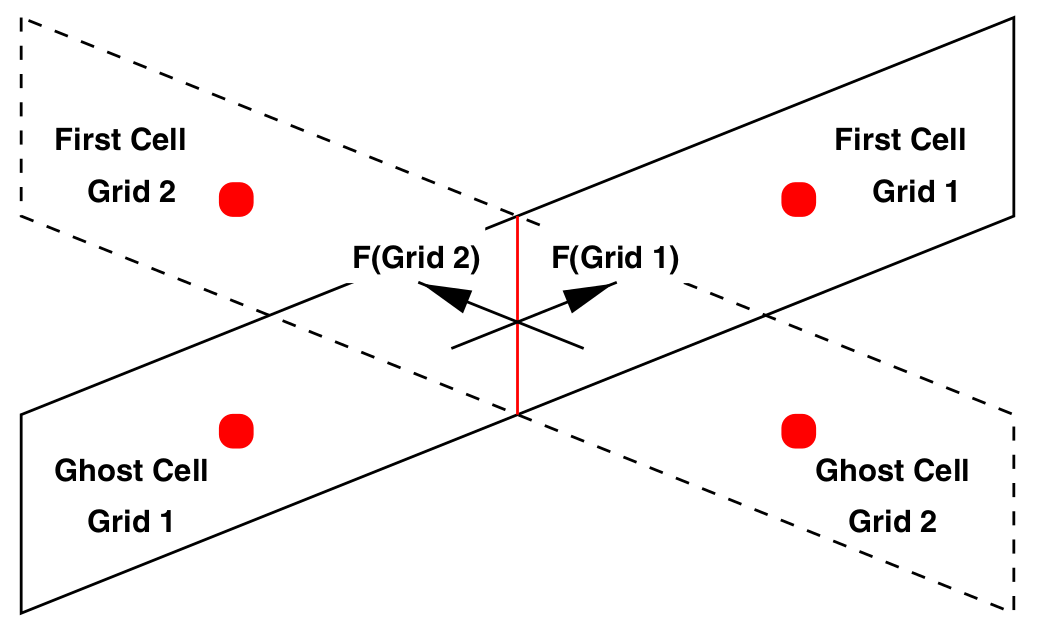
\includegraphics[width=0.5\linewidth]{flux_interface}
	\caption{Figure that illustrates the flux being computed twice on
		the cube edge, breaking the total mass conservation.
		Figure taken from \citet{ross:2006}.\label{chp5-fluxcube}}
\end{figure}
One common alternative used in the literature to handle the issue of values being defined twice at points on the
cube edges is to simply average the values (as seen in works such as \citet{ross:2006, chen:2008, chen:2021, mouallem:2023}).
When we are using flux averaging, we shall use the label \textbf{mf1}. When no mass fixer is used, we employ the label \textbf{mf0}.
 
\section{Numerical experiments}
\label{chp-cs-numexpadv}
This Section is dedicated to present the numerical experiments for the
advection equation on the sphere. In Table \ref{chp5-tab1} we present
the initial conditions (IC) and in Table \ref{chp5-vf} we present
the velocity fields (VF) considered.
In this section, we denote by $r$ the geodesic distance from any point $(\phi, \lambda)$ to a fixed point $(\phi_0, \lambda_0)$, expressed as
\begin{equation}
r=2R \arcsin{\bigg(
	\sqrt{\sin^2{\bigg(\frac{\phi-\phi_0}{2}\bigg)} + \cos{\phi}\cos{\phi_0}\cos^2{\bigg(\frac{\lambda-\lambda_0}{2}\bigg)}}\bigg)},
\end{equation}
where $R$ is the Earth radius. 
We shall made usage of the characteristic function $\chi_S$,  where $\chi_{S}(s)=1$ if $s \in S$, and $\chi_{S}(s)=0$ otherwise.
\begin{table}[!ht]
	\begin{tabular}{|c|l|l|}
		\hline
		IC name & \multicolumn{1}{c|}{$q_0$} \\ \hline
		IC1   & $\exp(b_0((X-X_0)^2+ (Y-Y_0)^2 + (Z-Z_0)^2))$ \\ \hline
		IC2   & $0.5+0.5(1+\cos{\frac{\pi r}{r_0}})\chi_{\{r<r_0\}}(r)$  \\ \hline
		IC3   & $0.1+0.9\chi_{\{r<r_0\}}(r)
		\chi_{\{|\lambda-\lambda_0|\leq0.05 \text{ or } \phi\leq\phi_0 \}}(\lambda,\phi)$ \\ \hline
		IC4   & $\exp(b_0[(X-X_1)^2+ (Y-Y_1)^2 + (Z-Z_1)^2]) + \exp(b_0[(X-X_2)^2+ (Y-Y_2)^2 + (Z-Z_2)^2])$ \\ \hline
	\end{tabular}
	\caption{Initial conditions considered in the numerical experiments (Figure \ref{chp5-ic}).}
	\label{chp5-tab1} 
\end{table}

\begin{table}[!ht]
	\begin{tabular}{|c|l|l|l|l|}
		\hline
		VF name & \multicolumn{1}{c|}{$u_\lambda(\lambda,\phi,t)$} & \multicolumn{1}{c|}{$v_\phi(\lambda,\phi,t)$}
		& \multicolumn{1}{c|}{$\Delta t^{(0)}$}	& \multicolumn{1}{c|}{CFL} \\ \hline
		VF1   & $u_0(\cos(\phi)\cos(\alpha) + \sin(\phi)\cos(\lambda)\sin(\alpha))$ 
		& $-u_0\sin(\lambda)\sin(\alpha)$ & 3600 & 0.95 \\ \hline
		VF2   & $u_0\sin^2(\lambda_p)\sin(2\phi)\cos(\frac{\pi t}{T})+u_0\cos\phi$ 
		& $u_0\sin(2\lambda_p)\cos(\phi)\cos(\frac{\pi t}{T})$& 1600 &0.73 \\ \hline
		VF3   & $-u_0\sin^2(\frac{\lambda+\pi}{2})\sin(2\phi)\cos^2(\phi)\cos(\frac{\pi t}{T})$ 
		& $\frac{u_0}{2}\sin(\lambda+\pi)\cos^3(\phi)\cos(\frac{\pi t}{T})$ & 6400 &0.91 \\ \hline
	\end{tabular}
	\caption{Velocity fields considered in the numerical experiments and their initial time step $\Delta t^{(0)}$ and CFL number.}
	\label{chp5-vf}
\end{table}

\begin{figure}[!htb]
	\centering
	\begin{subfigure}{0.45\textwidth}
		\centering
		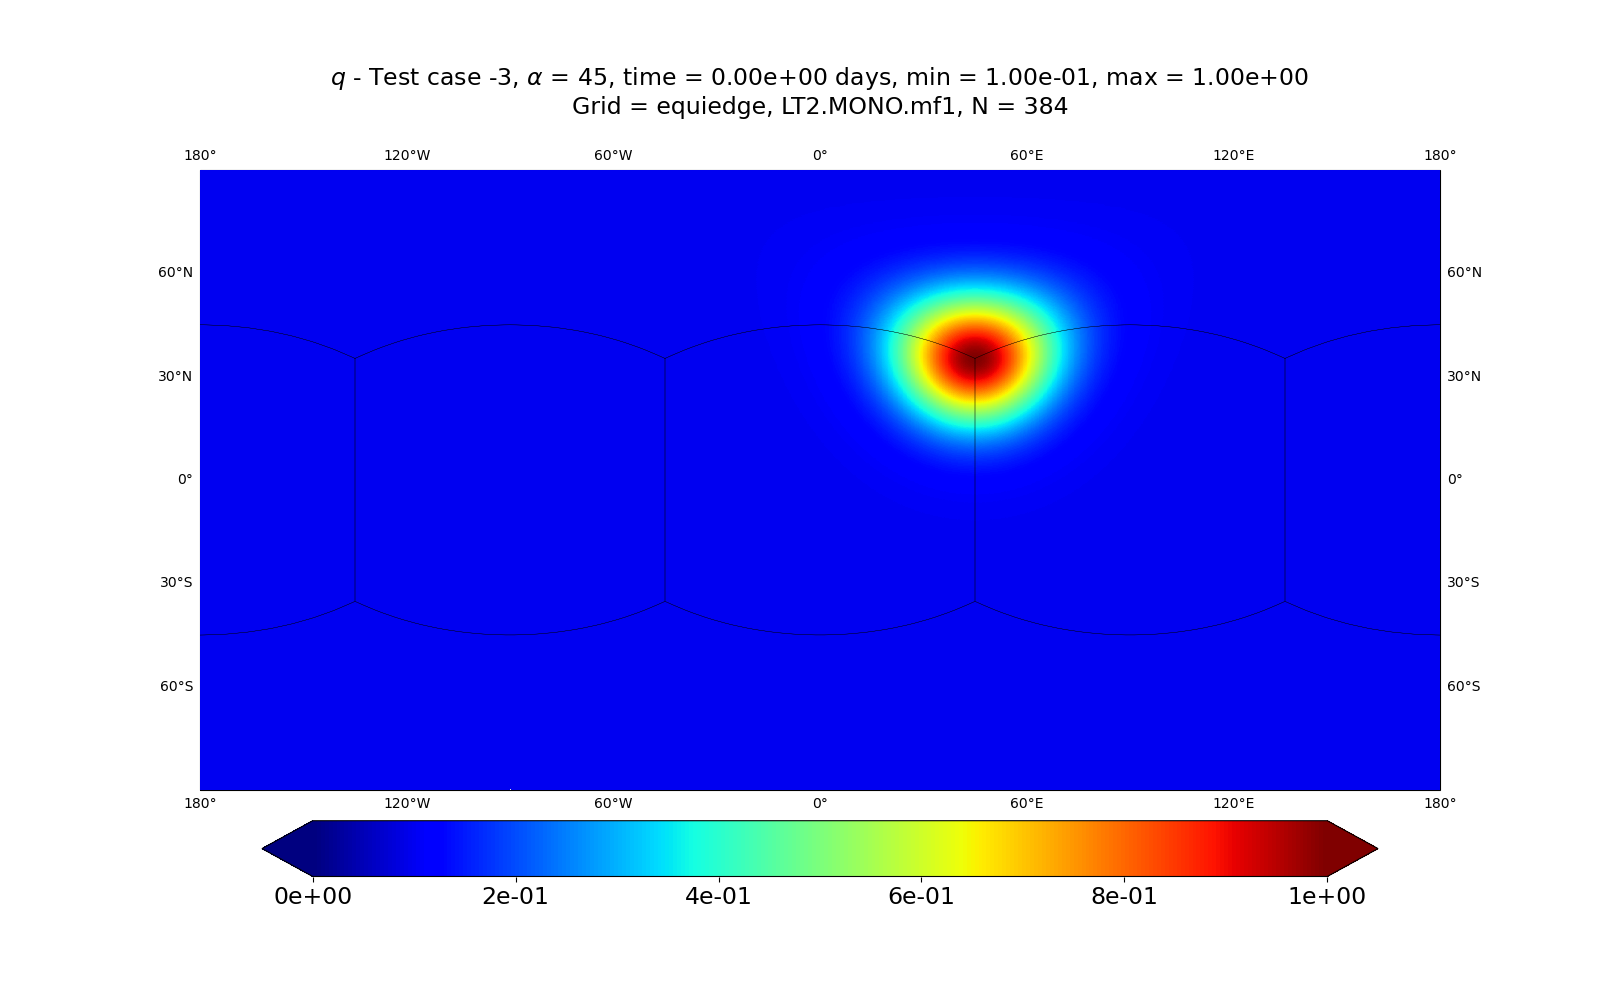
\includegraphics[width=0.9\linewidth]{h_tc-3_t0_alpha45_C384_g0_dg2_adv2_hord8_mf1_tf12}
		\caption{IC1. \label{chp5-ic1}}
	\end{subfigure}
	\begin{subfigure}{0.45\textwidth}
		\centering
		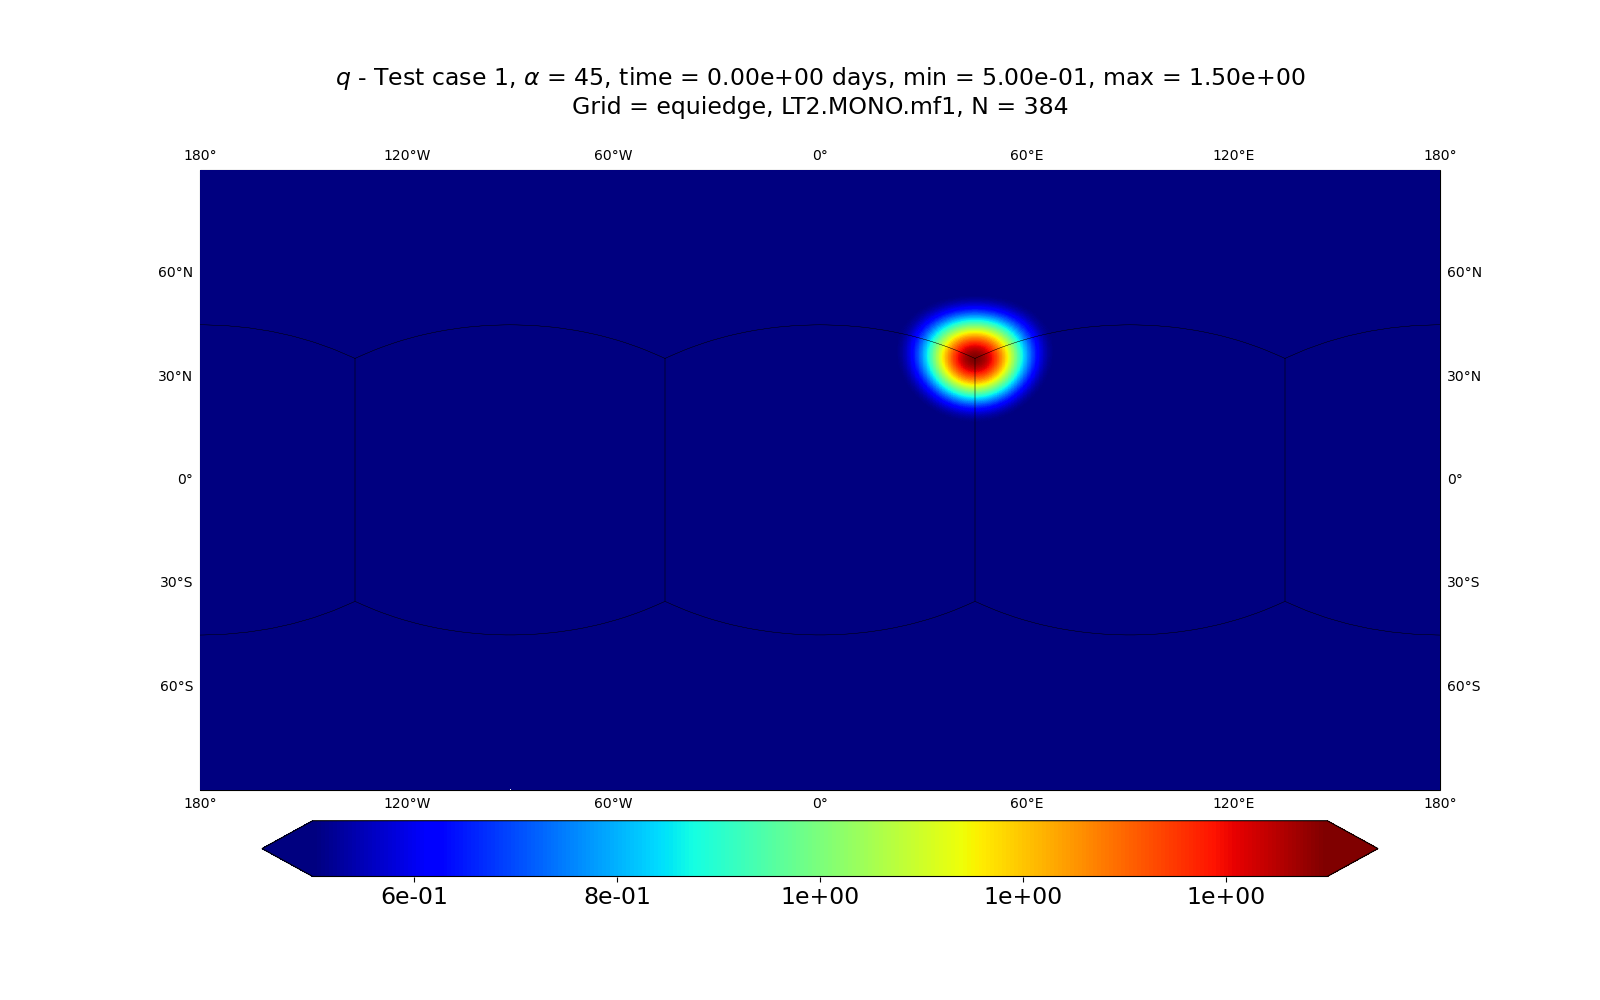
\includegraphics[width=0.9\linewidth]{h_tc1_t0_alpha45_C384_g0_dg2_adv2_hord8_mf1_tf12}
		\caption{IC2. \label{chp5-ic2}}
	\end{subfigure}

	\begin{subfigure}{0.45\textwidth}
	\centering
	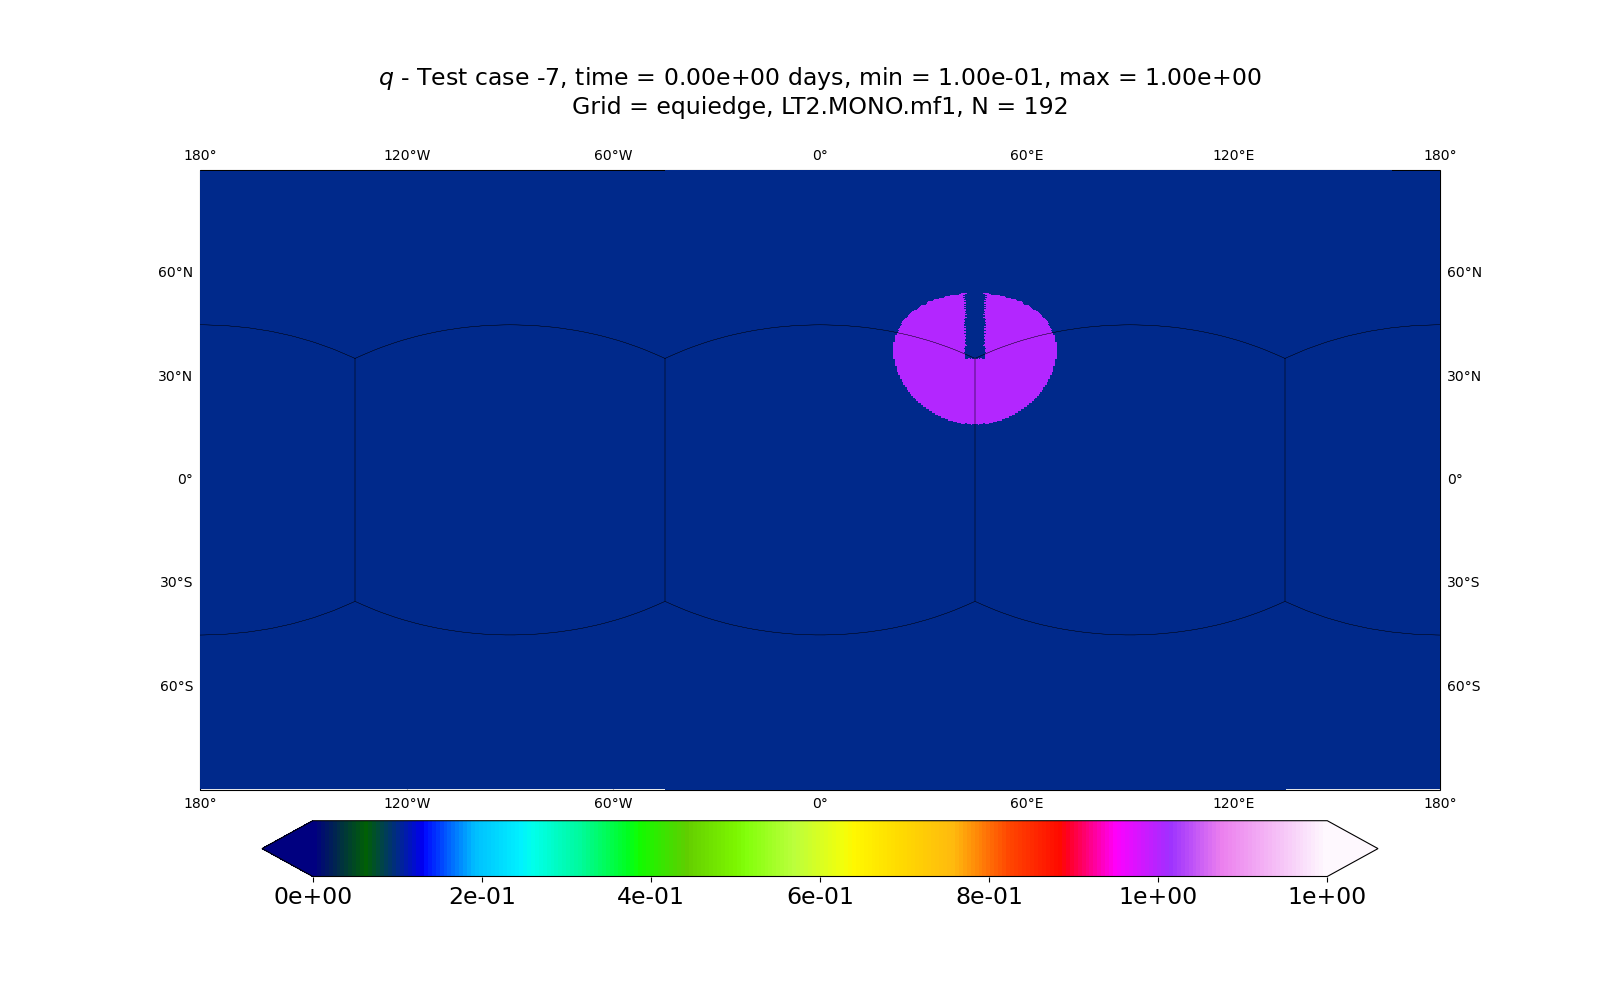
\includegraphics[width=0.9\linewidth]{h_tc-7_t0_alpha45_C192_g0_dg2_adv2_hord8_mf1_tf12}
	\caption{IC3. \label{chp5-ic3}}
    \end{subfigure}
    \begin{subfigure}{0.45\textwidth}
	\centering
	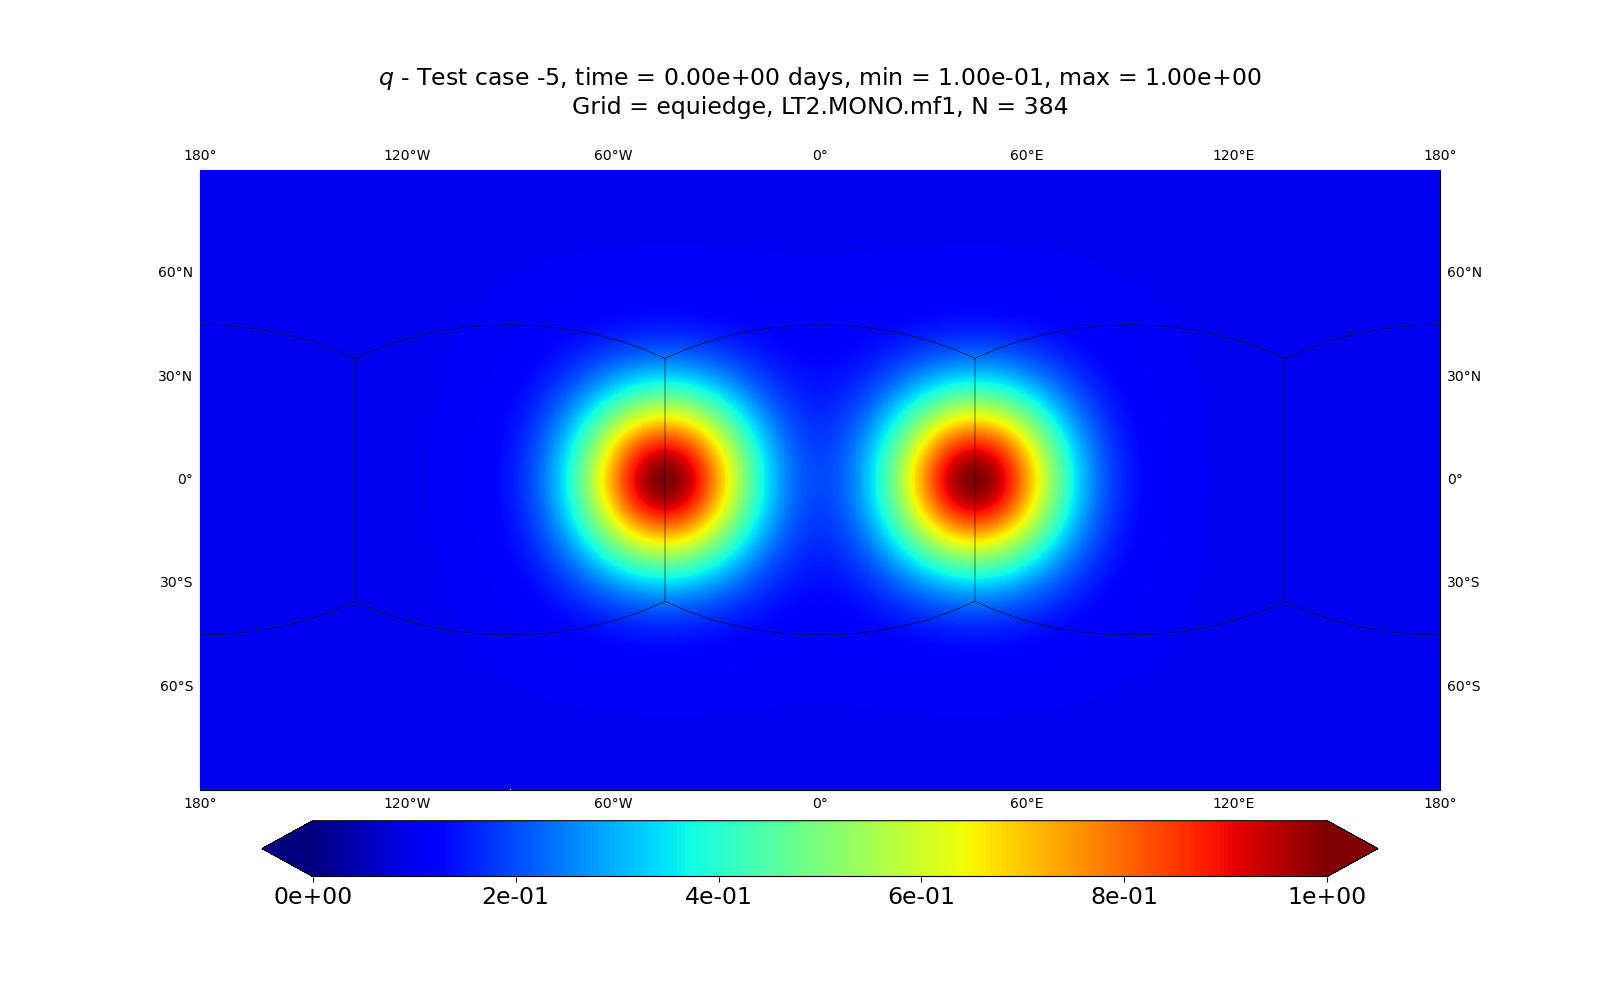
\includegraphics[width=0.9\linewidth]{h_tc-5_t0_alpha0_C384_g0_dg2_adv2_hord8_mf1_tf12}
	\caption{IC4. \label{chp5-ic4}}
    \end{subfigure}
	\caption{ Illustration of the initial conditions considered in this chapter (Table \ref{chp5-tab1}).\label{chp5-ic}}
\end{figure}


In Table \ref{chp5-tab1}, we have $(X_0,Y_0,Z_0)=(\frac{1}{\sqrt{3}},\frac{1}{\sqrt{3}},\frac{1}{\sqrt{3}})$, while 
$(X_1,Y_1,Z_1)$ and $(X_2,Y_2,Z_2)$ are the Cartesian coordinates of the latitude-longitude points
$(\lambda_1,\phi_1) = (-\frac{\pi}{4},0)$ and
$(\lambda_2,\phi_2) = ( \frac{\pi}{4},0)$, respectively.
IC1 represents a Gaussian hill centered at a cube corner and we set $b_0 = -10$.
IC2 represent a cosine bell centered at a cube corner, where $r_0 = \frac{R}{3}$, 
for $\lambda_0=\frac{\pi}{4}$ and $\phi_0 = \frac{\pi}{2}-\arccos{\big(\frac{1}{\sqrt{3}}\big)}$.
IC3 represent a slotted cylinder, based on  \citet{nair:2010}, where $r_0 = \frac{R}{3}$, 
for $\lambda_0=\frac{\pi}{4}$ and $\phi_0 = \frac{\pi}{2}-\arccos{\big(\frac{1}{\sqrt{3}}\big)}$,
and therefore the slotted cylinder is also centered at a cube corner.
IC4 represents two Gaussian hills as suggested by \citet{nair:2010} and we set $b_0 = -5$.
The initial conditions are shown in Figure \ref{chp5-ic}.

For the velocities provided in Table \ref{chp5-vf}, we adopt the following parameter values: 
$\alpha=\frac{\pi}{4}$, $\lambda_p=\lambda-\frac{2\pi t}{T}$, $T=12$ days (12$\times$86400 seconds) and $R$ is the Earth radius.
For VF1, VF2 and VF3, we use $u_0 = \frac{2\pi R}{T}$.
In this context, VF1 represents the non-divergent rotated zonal field introduced in \citet{will:1992}.
VF2 corresponds to the non-divergent deformational flow described in \citet{nair:2010},
and VF3 represents the divergent flow also presented in \citet{nair:2010}.
For all velocity fields presented here, the initial condition is equal to the final solution after 12 days.
Furthermore, for VF1, we can compute the exact solution at any time instant for any initial condition.
Therefore, we can analyze the temporal evolution of the error.
For an expression of the exact solution when using VF1 and a general initial condition, refer to \citet[Theorem 5.1, p. 155]{brachet:2018}.

We are going to consider the schemes LT-DP2 and PL-DP1 since these schemes yield better results on planar simulations (Section \ref{sec-ds-exp}).
For a shorter notation, we shall denote LT-DP2 and PL-DP1 by \textbf{LT} and \textbf{PL} advection schemes. 
These schemes will be tested using the unlimited PPM  and the monotonic PPM scheme.
As we mentioned in Section \ref{sec-metricppm}, the PL scheme needs the \textbf{mt1} 
metric term formulation for the 1D flux operators to eliminate the splitting error for a constant scalar field.
For the LT scheme, we shall use the \textbf{mt0} metric term formulation because for this scheme, 
we do not have the constraint of eliminating the splitting error for a constant scalar field. 
Furthermore, this formulation makes the LT scheme much more accurate, while \textbf{mt1} for LT makes it first-order.
We are also going to consider the simulations without mass fixer (\textbf{mf0}) and with flux averaging at
cube edges (\textbf{mf1}) to investigate the impact of flux averaging on accuracy.
Additionally, we are using the duo-grid to fill the ghost cell values using cubic polynomials.
The reader may refer to \citet{mouallem:2023} for a comparison between results on the duo-grid versus the kinked grid.
Both equi-edge (g0, Section \ref{cs-equiedge}) and equiangular grids (g2, Section \ref{cs-equiangular})
using the spherical midpoints formulation (Section \ref{cs-geo}) are going to be consider in this Section.

To compute the convergence, consider cubed-sphere grids with value of $N_k =  48\times2^{k}$,
and $\Delta t^{(k)} = \frac{\Delta t^{(k)}}{2^k}$, $k=0, \ldots, 4$, where
the value of $\Delta t^{(0)}$ in Table \ref{chp5-vf} for each VF.
The relative error in the $p$-norm (Equation \eqref{chp-advcs-pnorm})
and the convergence rate are defined as in Section \ref{chp-adv1d-sec-numerical-exp}.

\newpage
\subsection{Advection of one Gaussian hill through the rotated zonal wind}
As a first test case, we consider the advection of the Gaussian hill given by IC1 using 
the rotated zonal wind VF1.
In Figure \ref{chp-advcs-sec-exp-adv2}, we illustrate how the Gaussian hill is advected and passes over 4 cube corners, 
eventually returning to its initial position. 
\begin{figure}[!htb]
	\centering
	\begin{subfigure}{0.45\textwidth}
		\centering
		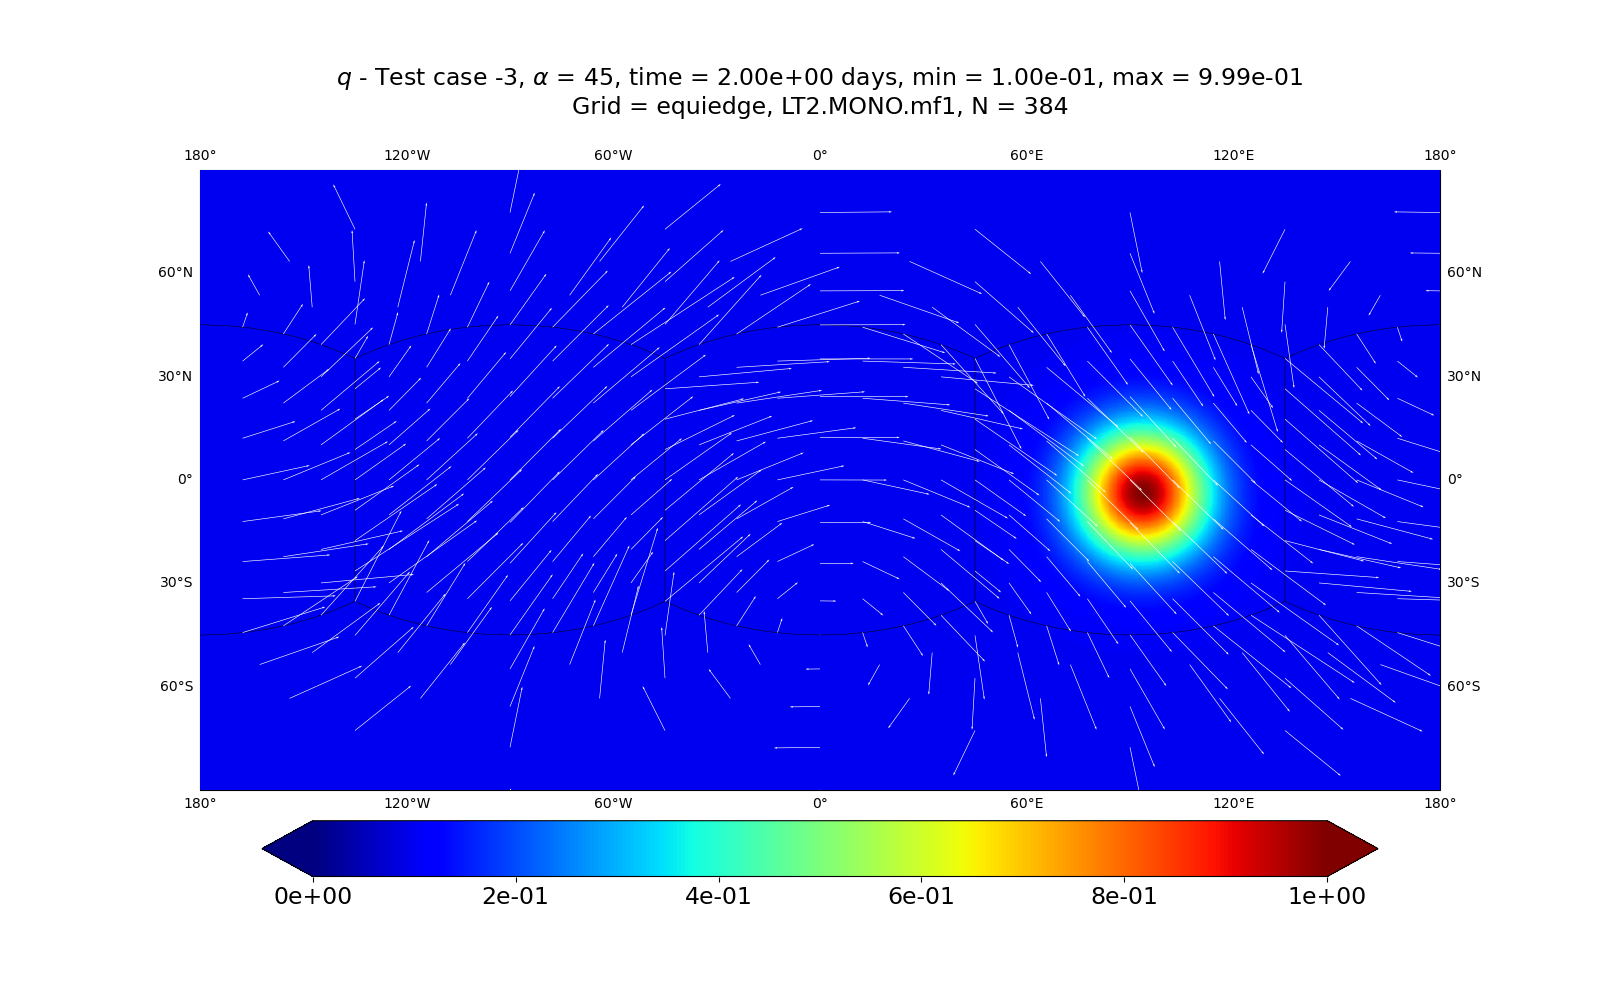
\includegraphics[width=1\linewidth]{h_tc-3_t2_alpha45_C384_g0_dg2_adv2_hord8_mf1_tf12}
		\caption{$t=2$ days.\label{chp-advcs-sec-exp-adv2-a}}
	\end{subfigure}
	\begin{subfigure}{0.45\textwidth}
		\centering
		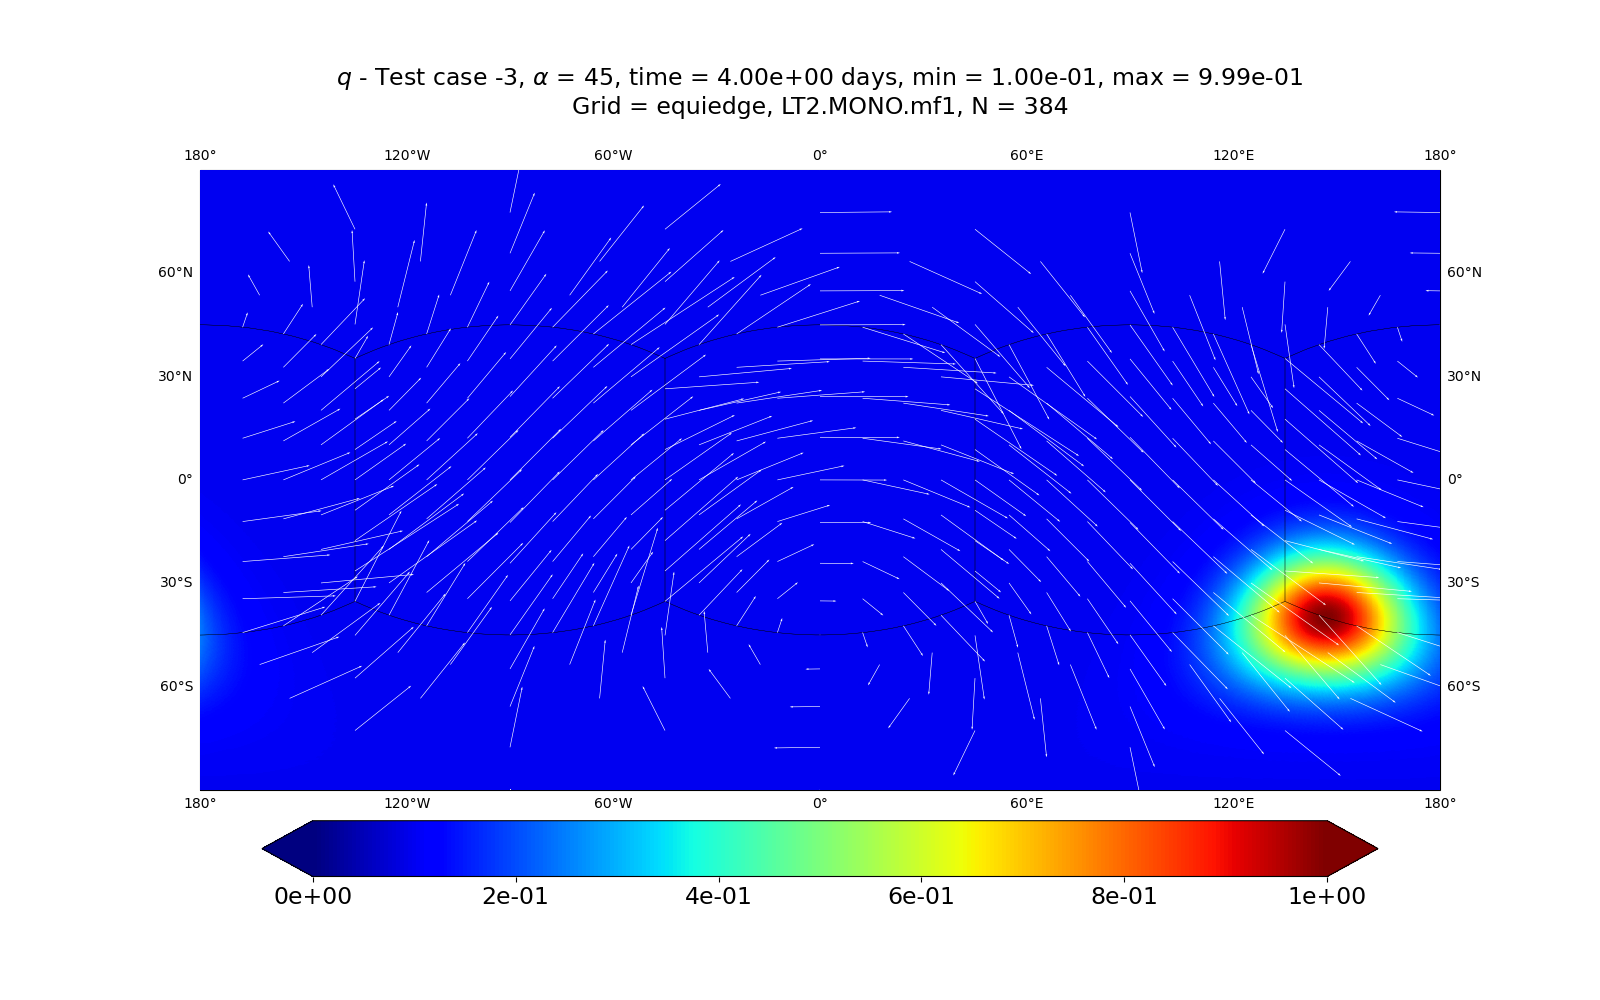
\includegraphics[width=1\linewidth]{h_tc-3_t4_alpha45_C384_g0_dg2_adv2_hord8_mf1_tf12}
		\caption{$t=4$ days.\label{chp-advcs-sec-exp-adv2-b}}
	\end{subfigure}

	\begin{subfigure}{0.45\textwidth}
		\centering
		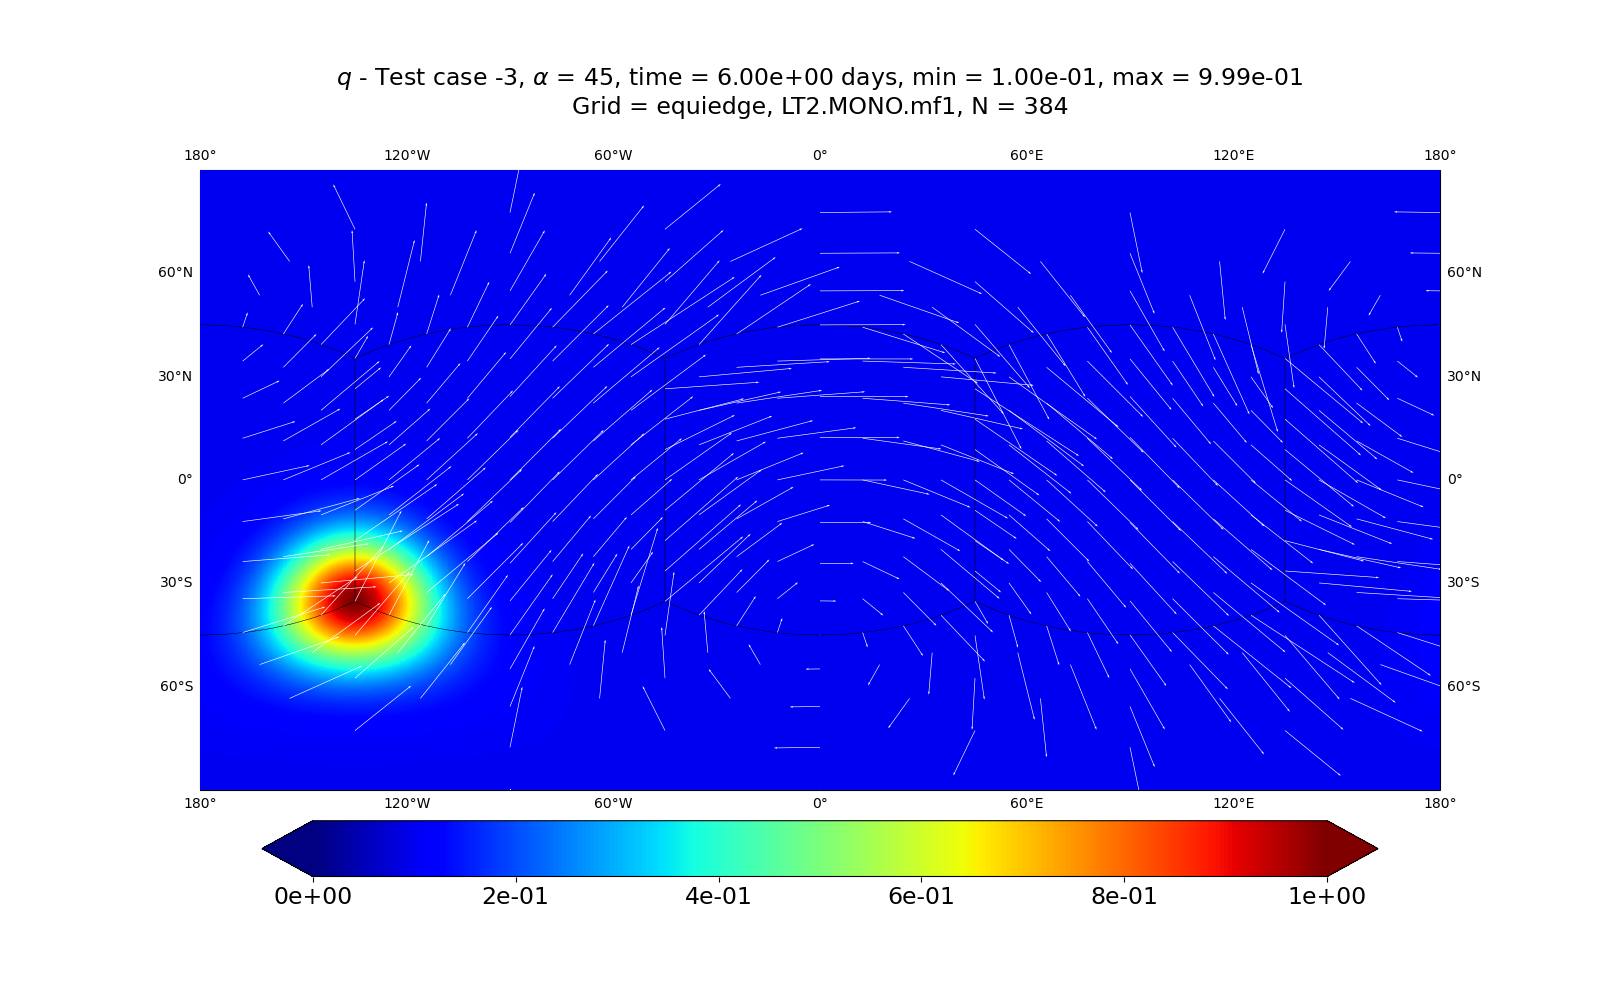
\includegraphics[width=1\linewidth]{h_tc-3_t6_alpha45_C384_g0_dg2_adv2_hord8_mf1_tf12}
		\caption{$t=6$ days.\label{chp-advcs-sec-exp-adv2-c}}
	\end{subfigure}	
	\begin{subfigure}{0.45\textwidth}
		\centering
		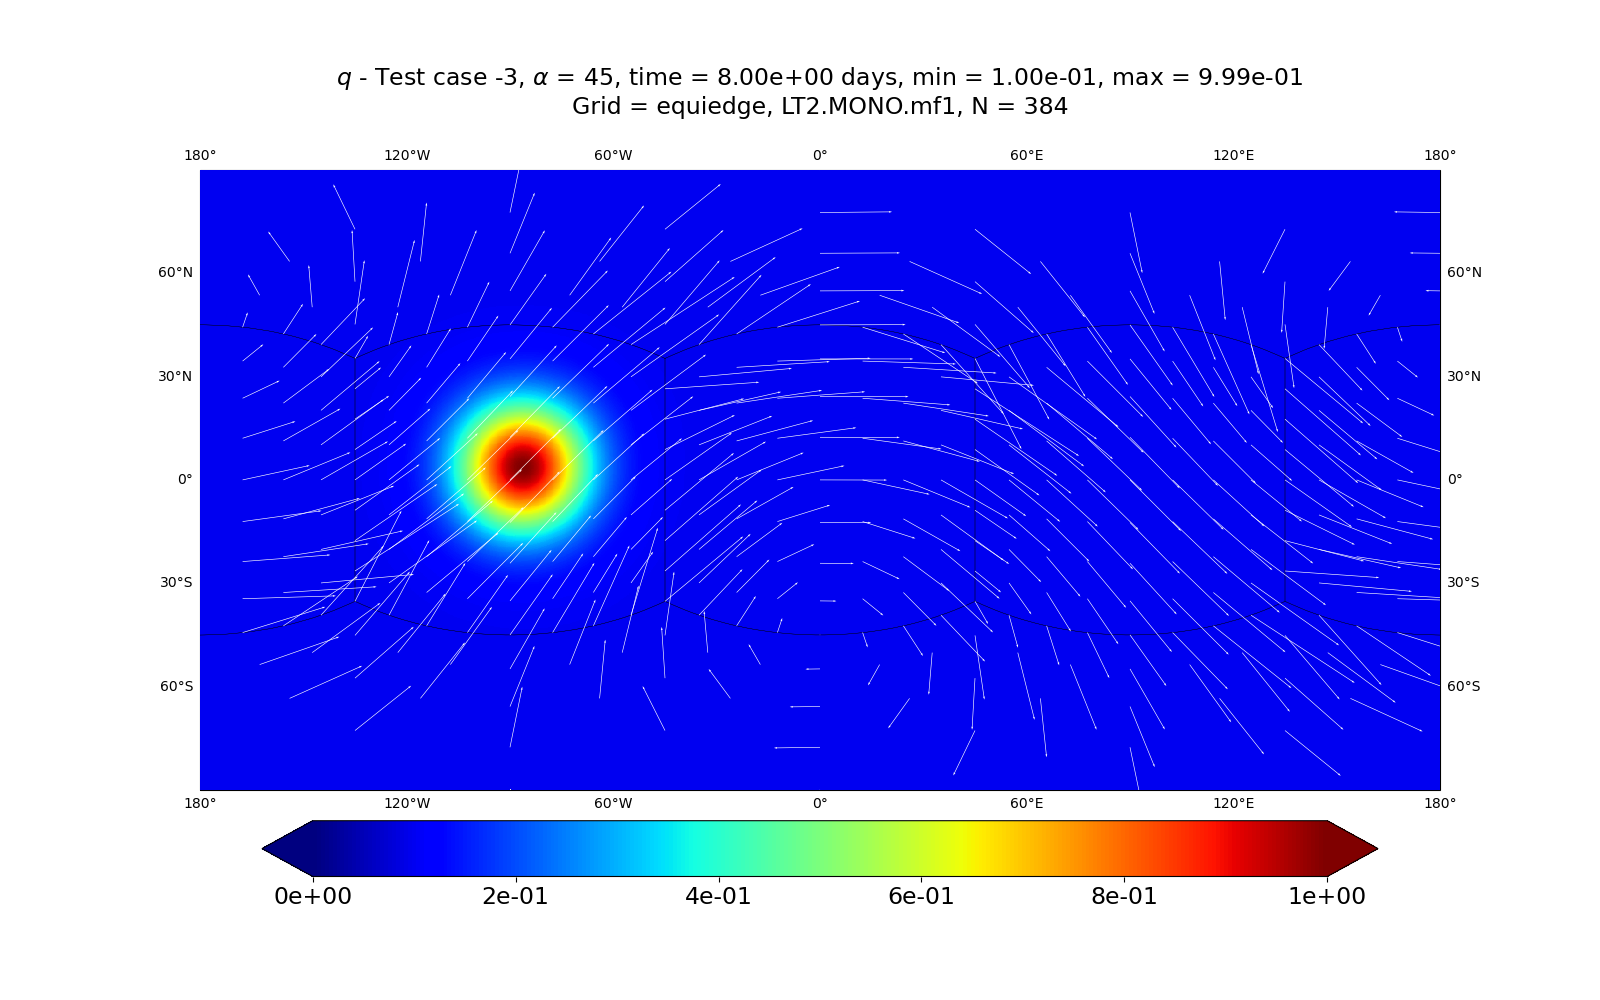
\includegraphics[width=1\linewidth]{h_tc-3_t8_alpha45_C384_g0_dg2_adv2_hord8_mf1_tf12}
		\caption{$t=8$ days.\label{chp-advcs-sec-exp-adv2-d}}
	\end{subfigure}

	\begin{subfigure}{0.45\textwidth}
		\centering
		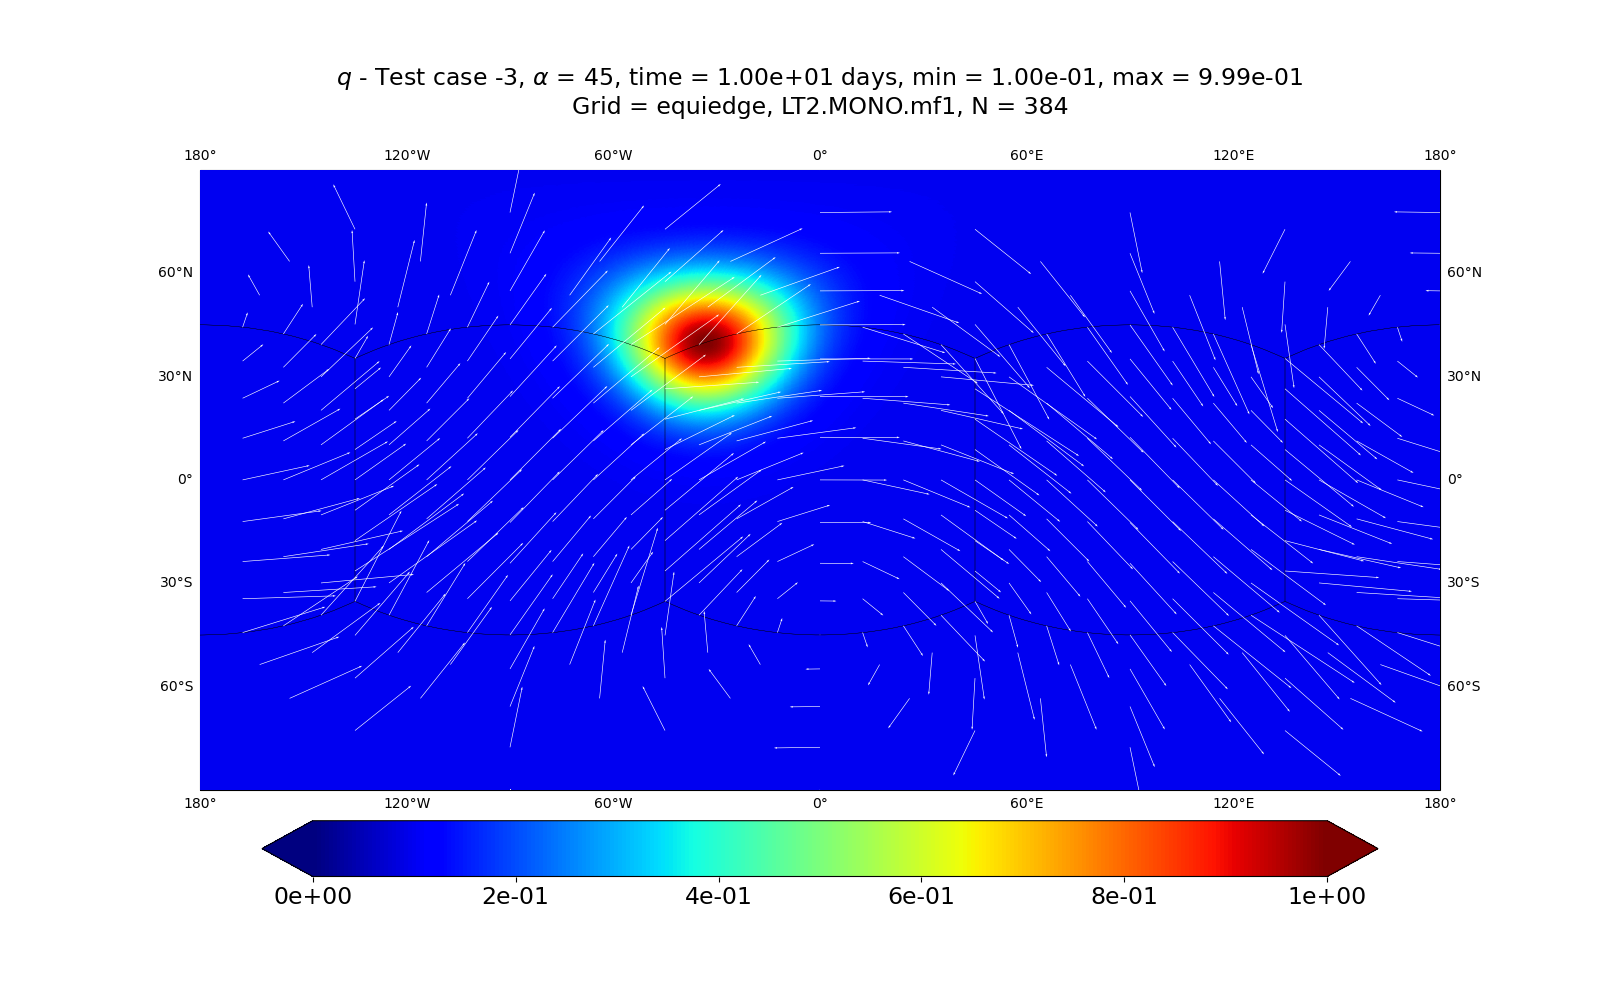
\includegraphics[width=1\linewidth]{h_tc-3_t10_alpha45_C384_g0_dg2_adv2_hord8_mf1_tf12}
		\caption{$t=10$ days.\label{chp-advcs-sec-exp-adv2-e}}
	\end{subfigure}
	\begin{subfigure}{0.45\textwidth}
		\centering
		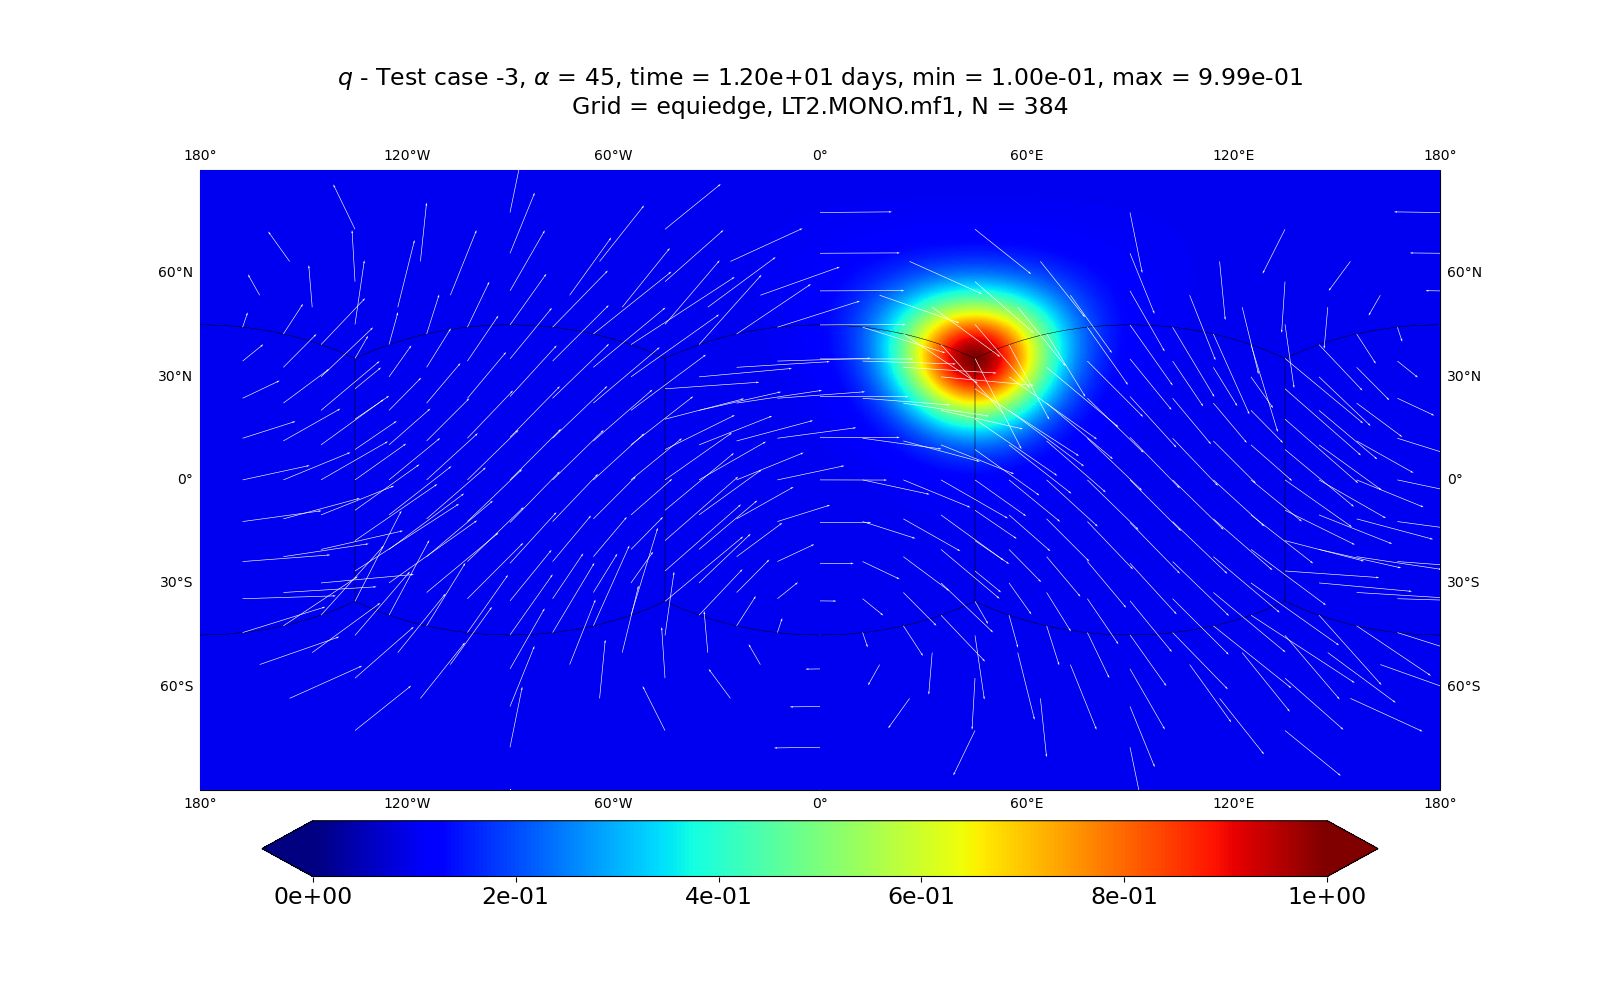
\includegraphics[width=1\linewidth]{h_tc-3_t12_alpha45_C384_g0_dg2_adv2_hord8_mf1_tf12}
		\caption{$t=12$ days.\label{chp-advcs-sec-exp-adv2-f}}
	\end{subfigure}
	\caption{Advection experiment results using the Gaussian hill at a cube corner (IC1, Table \ref{chp5-ic}) and 
		the rotated zonal wind (VF1, Table \ref{chp5-vf}).
		These figures show the advected profile after
		2 \eqref{chp-advcs-sec-exp-adv2-a}, 
		4  \eqref{chp-advcs-sec-exp-adv2-b},
		6  \eqref{chp-advcs-sec-exp-adv2-c},
		8  \eqref{chp-advcs-sec-exp-adv2-d},
		10  \eqref{chp-advcs-sec-exp-adv2-e},
		and 12  \eqref{chp-advcs-sec-exp-adv2-f} days.
		We are using the LT-MONO-mf1 scheme on the equi-edge grid (g0) with $N=384$. \label{chp-advcs-sec-exp-adv2}}
\end{figure}

The goal of this test is to observe the ability of all schemes and grids to perform this test without creating
larger errors or grid-imprinting when the Gaussian hill reaches a corner.
In fact, in Figure \ref{chp-advcs-sec-exp-adv2-evol-linf} we show how the error evolves with time over 12 days in the $L_{\infty}$ norm for $N=384$.
Similarly, Figure \ref{chp-advcs-sec-exp-adv2-evol-l2} shows the error evolution over time in the $L_2$ norm.
Both figures use green lines to represent the PL scheme and blue lines to represent the LT scheme.
Light colors denote cases where the mass fixer is not used, while dark colors represent cases where it is used. 
Dashed lines represent the monotonic while solid lines represent the unlimited PPM.

In terms of the $L_2$ norm, as shown in Figure \ref{chp-advcs-sec-exp-adv2-evol-l2}, 
no spikes are observed in the graphs corresponding to the days when the Gaussian passes over a corner.
Another conclusion is that the mass fixer does not have too much impact on error evolution when the monotonic scheme is used.
However, from Figure \ref{chp-advcs-sec-exp-adv2-evol-linf} we can see some small spikes in the $L_{\infty}$ error
on the equi-edge grid (g0) when using the PL and LT schemes, which is less pronounced on the equiangular grid.
\begin{figure}[!htb]
	\centering
	\begin{subfigure}{0.45\textwidth}
	\centering
	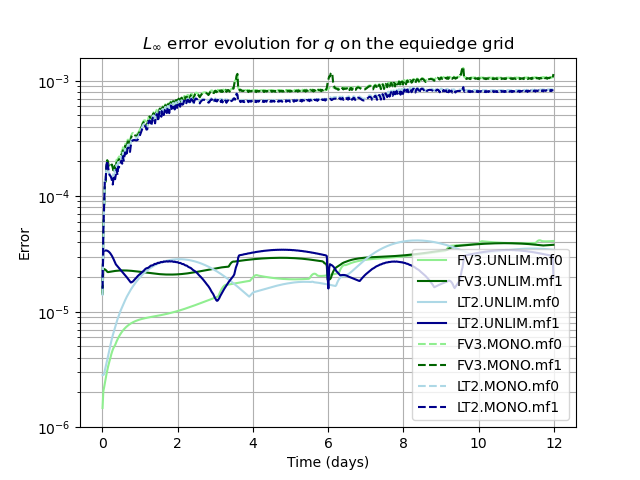
\includegraphics[width=1\linewidth]{tc-3_C384_linf_errors_equiedge}
	\caption{Equi-edge grid}
\end{subfigure}
\begin{subfigure}{0.45\textwidth}
	\centering
	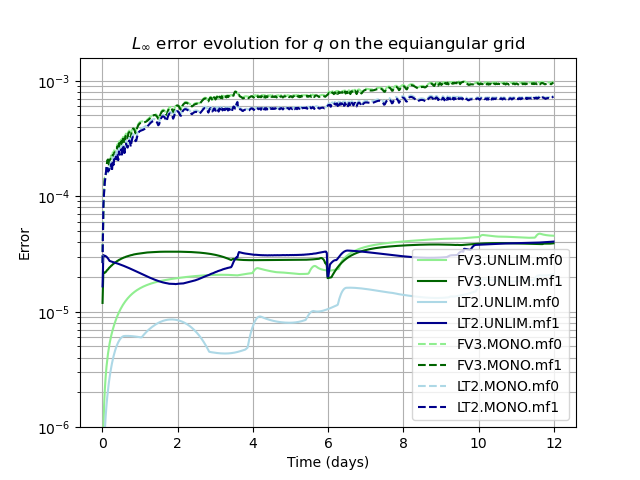
\includegraphics[width=1\linewidth]{tc-3_C384_linf_errors_equiangular}
	\caption{Equiangular grid}
\end{subfigure}
	\caption{
		$L_{\infty}$ error evolution for IC1 (Table \ref{chp5-ic}) and VF1 (Table \ref{chp5-vf}) 
		on the equi-edge grid (a) and on the equiangular grid (b) grids for 12 days and $N=384$.
		Blue lines indicate the use of the LT scheme, while green lines represent the PL scheme.
		Solid lines represent the results with the unlimited PPM (UNLIM) scheme, whereas dashed lines represent the results with the monotonic (MONO).
		Light colors show the result without mass fixer (mf0), whereas dark colors show the results with flux averaging (mf1).
		\label{chp-advcs-sec-exp-adv2-evol-linf}}
\end{figure}

\begin{figure}[!htb]
	\centering
	\begin{subfigure}{0.45\textwidth}
		\centering
		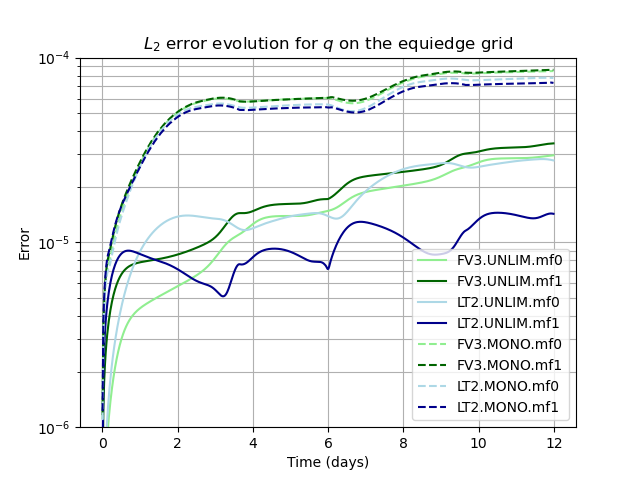
\includegraphics[width=1\linewidth]{tc-3_C384_l2_errors_equiedge}
		\caption{Equi-edge grid}
	\end{subfigure}
	\begin{subfigure}{0.45\textwidth}
		\centering
		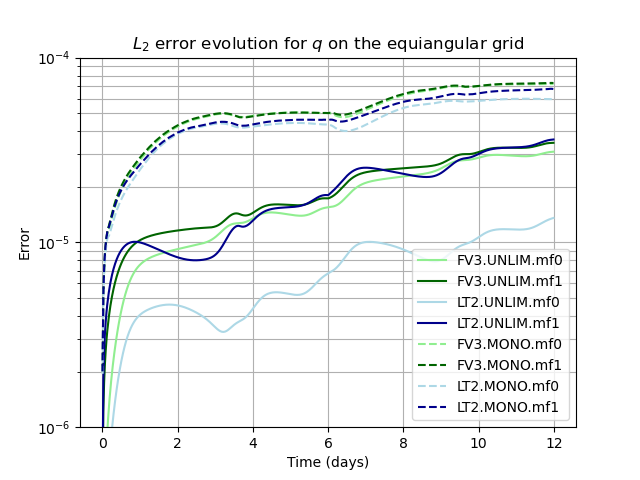
\includegraphics[width=1\linewidth]{tc-3_C384_l2_errors_equiangular}
		\caption{Equiangular grid}
	\end{subfigure}
	\caption{As Figure \ref{chp-advcs-sec-exp-adv2-evol-linf} but using the $L_2$ error.\label{chp-advcs-sec-exp-adv2-evol-l2}}
\end{figure}

\newpage
Indeed, Figure \ref{chp-advcs-sec-exp-adv2-errors-0} shows the final error at a cube corner for the equi-edge grid (g0), 
and Figure \ref{chp-advcs-sec-exp-adv2-errors-2} shows it for the equiangular grid (g2).
The results without a mass fixer are very similar and are not shown here. 
We can observe that the errors for PL are larger at the corners
(Figures \ref{chp-advcs-sec-exp-adv2-errors-0a} and \ref{chp-advcs-sec-exp-adv2-errors-2a}) 
than the corner errors of the LT scheme (Figures \ref{chp-advcs-sec-exp-adv2-errors-0b} and \ref{chp-advcs-sec-exp-adv2-errors-2b}).
Additionally, the equi-edge grid (g0) and the equiangular grid (g2) yield similar results for both schemes,
with the equi-edge grid resulting in smaller maximum errors.
\begin{figure}[!htb]
	\centering
	\begin{subfigure}{0.45\textwidth}
		\centering
		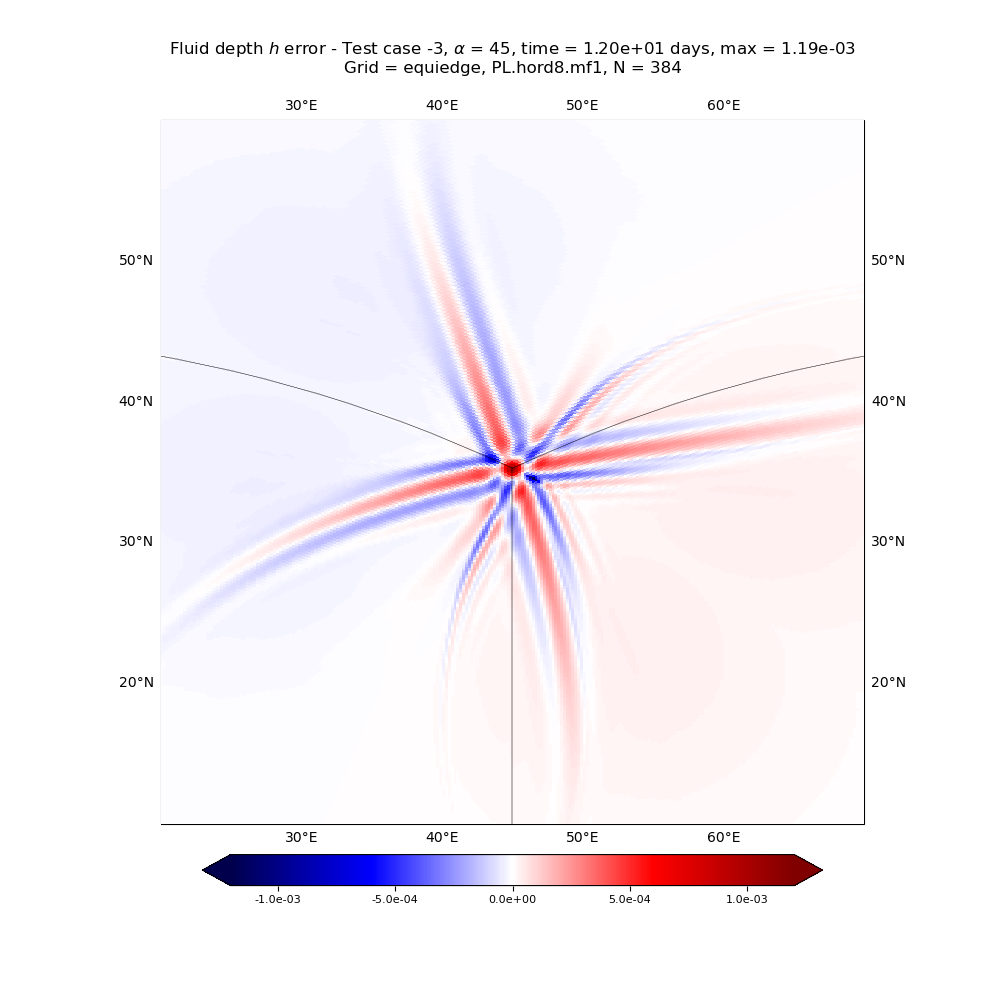
\includegraphics[width=1\linewidth]{h_error_tc-3_t12_alpha45_C384_g0_dg2_adv1_hord8_mf1_tf12}
		\caption{PL scheme - max = $1.19 \times 10^{-3}$.\label{chp-advcs-sec-exp-adv2-errors-0a}}
	\end{subfigure}
	\begin{subfigure}{0.45\textwidth}
		\centering
		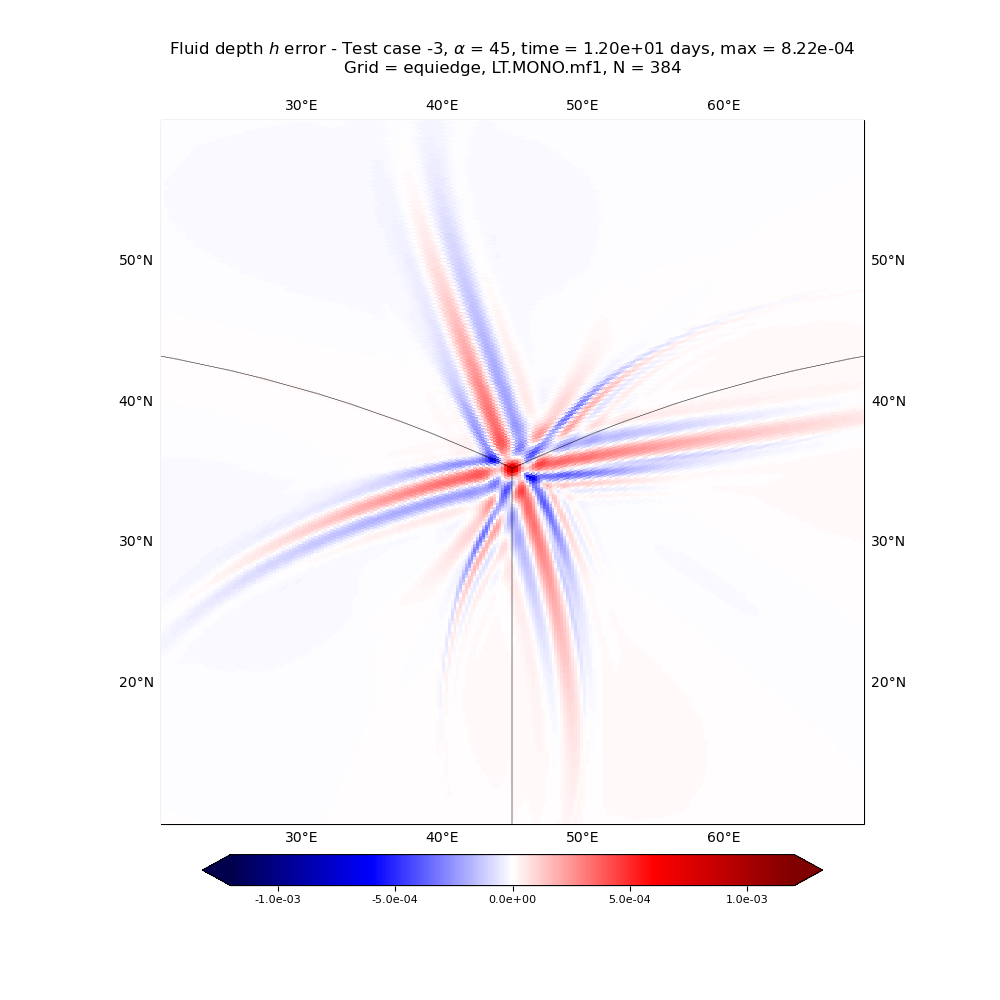
\includegraphics[width=1\linewidth]{h_error_tc-3_t12_alpha45_C384_g0_dg2_adv2_hord8_mf1_tf12}
		\caption{LT scheme - max = $8.22 \times 10^{-4}$.\label{chp-advcs-sec-exp-adv2-errors-0b}}
	\end{subfigure}
	\caption{
		Advection experiment errors at a cube corner using the Gaussian hill (IC1, Table \ref{chp5-ic}) and  
		the rotated zonal wind (VF1, Table \ref{chp5-vf}) after 12 days, using the monotonic scheme (MONO) 
		with PL (left) and LT schemes (right) on the equi-edge grid (g0) with $N=384$. 
		\label{chp-advcs-sec-exp-adv2-errors-0}}
\end{figure}
\begin{figure}[!htb]
	\centering
	\begin{subfigure}{0.45\textwidth}
		\centering
		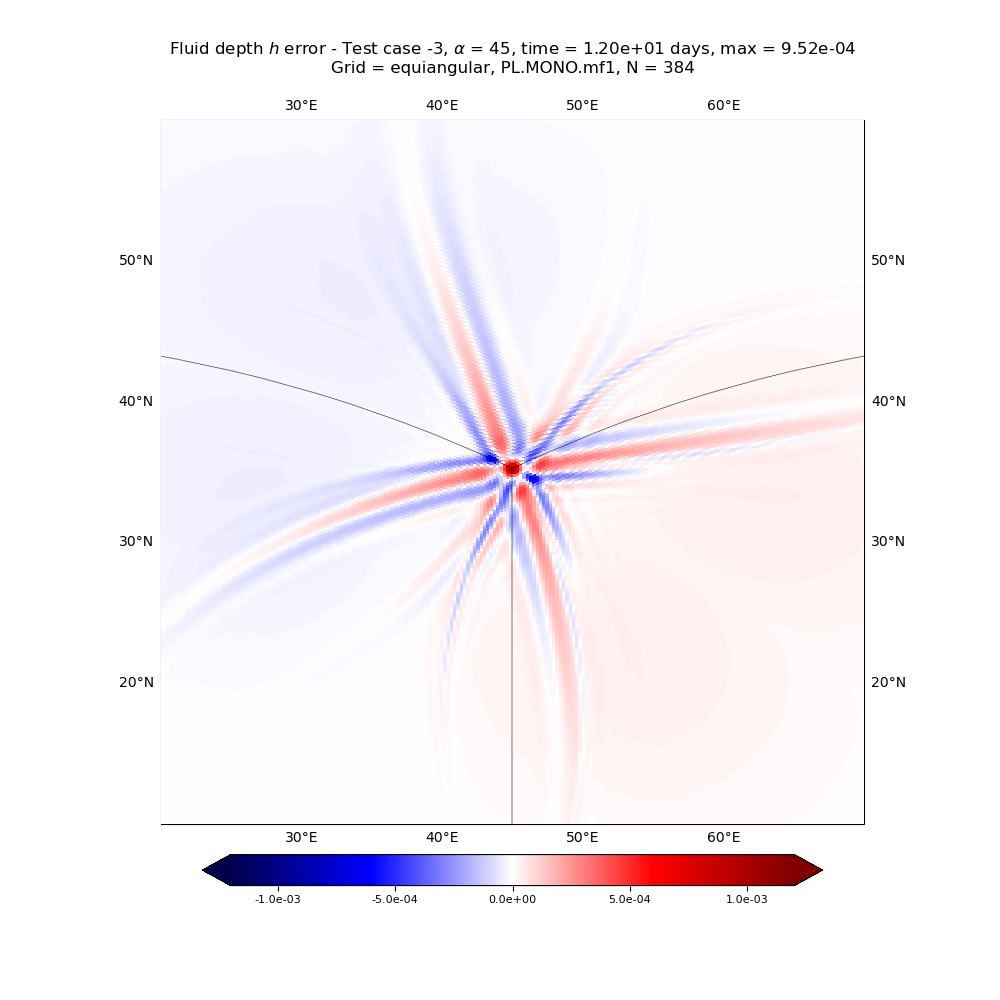
\includegraphics[width=1\linewidth]{h_error_tc-3_t12_alpha45_C384_g2_dg2_adv1_hord8_mf1_tf12}
		\caption{PL scheme - max = $9.52 \times 10^{-4}$.\label{chp-advcs-sec-exp-adv2-errors-2a}}
	\end{subfigure}
	\begin{subfigure}{0.45\textwidth}
		\centering
		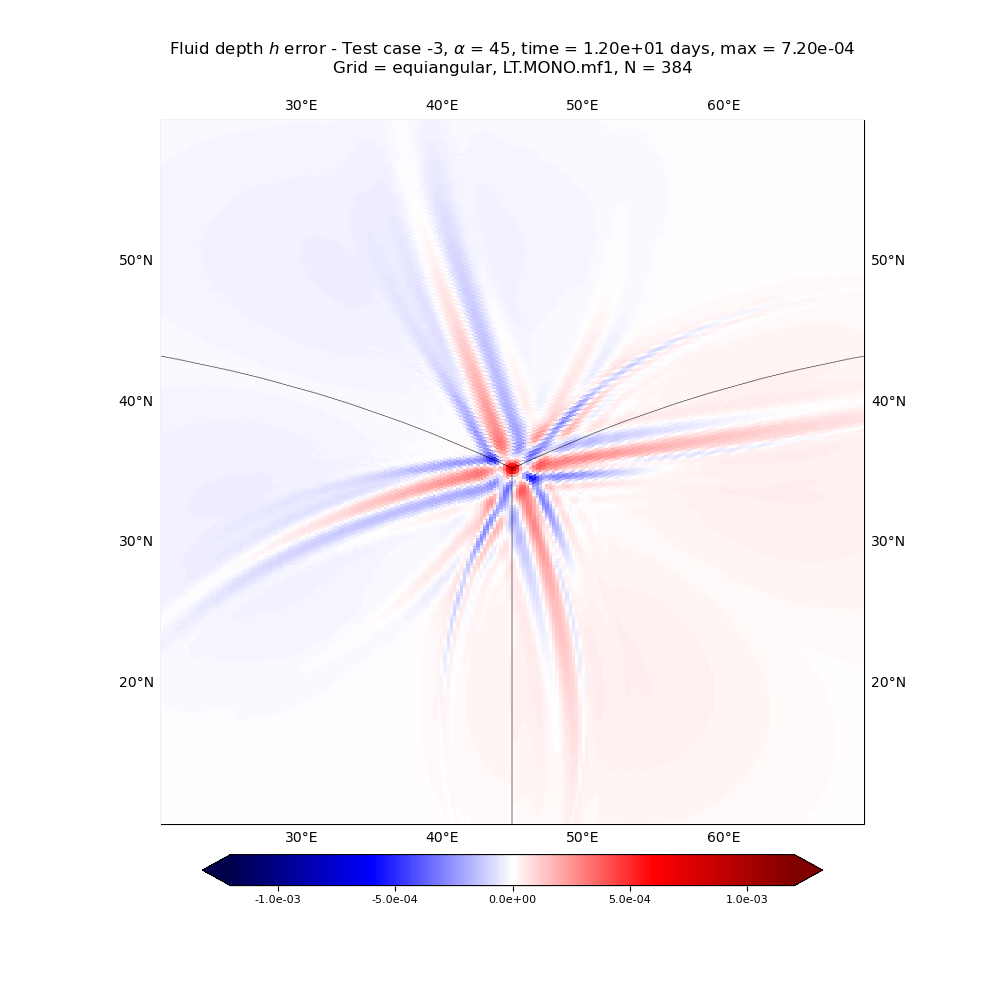
\includegraphics[width=1\linewidth]{h_error_tc-3_t12_alpha45_C384_g2_dg2_adv2_hord8_mf1_tf12}
		\caption{LT scheme - max = $7.20 \times 10^{-4}$.\label{chp-advcs-sec-exp-adv2-errors-2b}}
	\end{subfigure}
	\caption{As Figure \ref{chp-advcs-sec-exp-adv2-errors-0} but using the equiangular grid (g2).\label{chp-advcs-sec-exp-adv2-errors-2}}
\end{figure}


\newpage
Finally, in Figures \ref{chp-advcs-sec-exp-adv2-linf} and \ref{chp-advcs-sec-exp-adv2-l2} we show the error convergence in $L_{\infty}$ and $L_{2}$ norms.
We can observe that all schemes with the unlimited PPM (UNLIM) achieve second-order accuracy as expected.
However, for MONO, the order is reduced, which is also expected.
Additionally, we can see that MONO with LT has smaller errors when comparing the blue dashed lines with the green dashed lines, 
for both $L_{\infty}$ and $L_{2}$ norms on both equi-edge grid (g0) and the equiangular grid (g2), indicating that LT is slightly more accurate.
In general, the errors of g0 are slightly smaller than those of g2.
\begin{figure}[!htb]
	\centering
	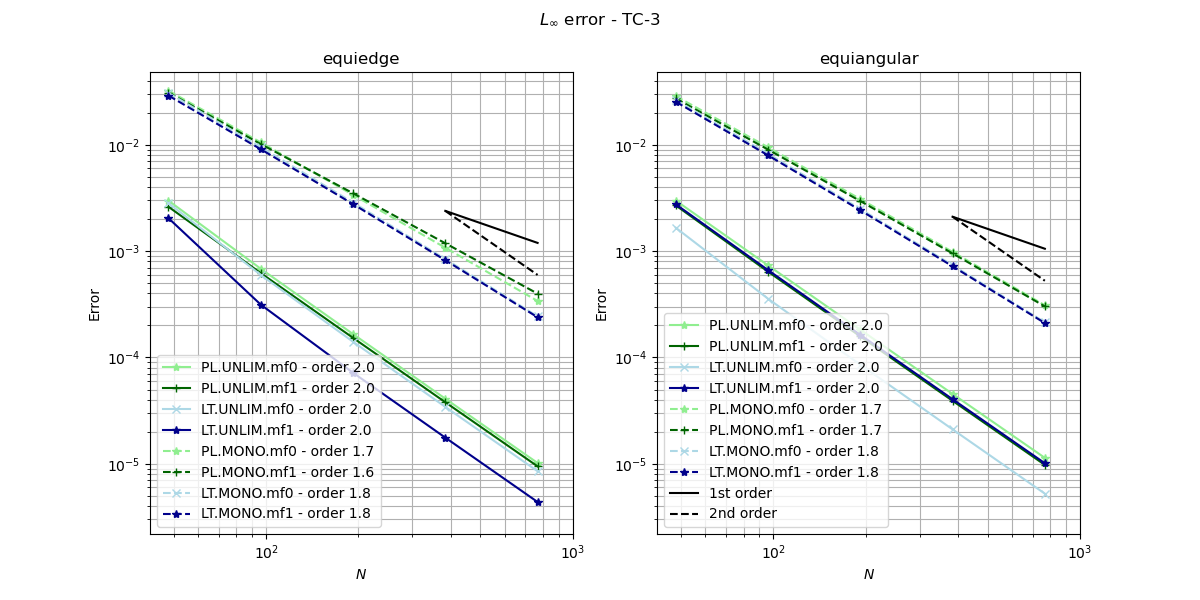
\includegraphics[width=0.9\linewidth]{linferror_tc-3_alpha45}
	\caption{
$L_{\infty}$ error convergence for the advection on the sphere test using the Gaussian hill at cube a corner (IC1, Table \ref{chp5-ic}) and 
the rotated zonal wind  (VF1, Table \ref{chp5-vf}) on the equi-edge grid (g0, left) 
and on the equiangular grid (g2, right) after 12 days.
Blue lines indicate the use of the LT scheme, while green lines represent the PL scheme.
Solid lines represent the results with the unlimited PPM (UNLIM) scheme, whereas dashed lines represent the results with the monotonic PPM (MONO).
Light colors show the result without mass fixer (mf0), whereas dark colors show the results with flux averaging (mf1).\label{chp-advcs-sec-exp-adv2-linf}}
\end{figure}

\begin{figure}[!htb]
	\centering
	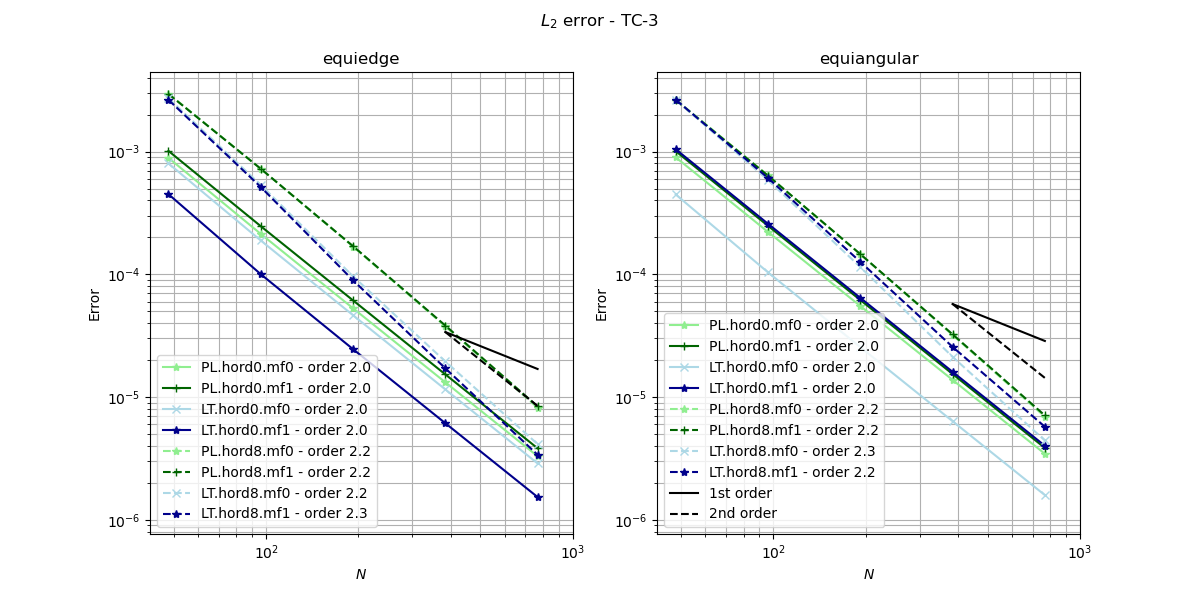
\includegraphics[width=0.9\linewidth]{l2error_tc-3_alpha45}
	\caption{As Figure \ref{chp-advcs-sec-exp-adv2-linf} but considering the $L_2$ norm. \label{chp-advcs-sec-exp-adv2-l2}}
\end{figure}

\newpage
\subsection{Advection of a cosine bell hill through the rotated zonal wind}
As the second test case, we consider the advection of the cosine bell given by IC2 using the rotated zonal wind VF1.
The cosine bell is advected and passes over 4 cube corners, very similarly to the Gaussian hill, as shown in Figure \ref{chp-advcs-sec-exp-adv2}.
The major difference between IC1 and IC2 is that IC1 is a smooth function while IC2 is only continuous.
Then, we may compare how both schemes handle a non-differentiable function.
For $N=384$, the temporal evolution of the errors is very similar to that of IC1
(Figures \ref{chp-advcs-sec-exp-adv2-evol-linf} and \ref{chp-advcs-sec-exp-adv2-evol-l2}) and is omitted here.
\begin{figure}[!htb]
	\centering
	\begin{subfigure}{0.35\textwidth}
		\centering
		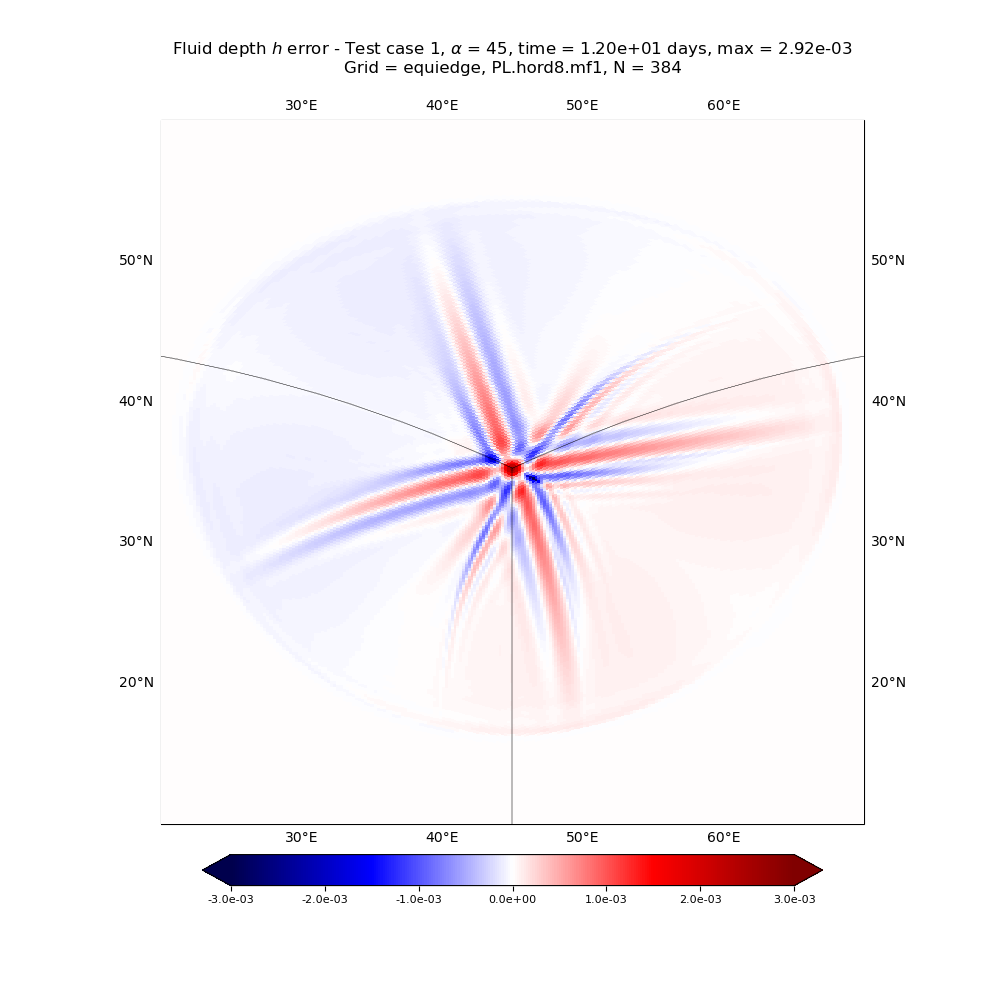
\includegraphics[width=1\linewidth]{h_error_tc1_t12_alpha45_C384_g0_dg2_adv1_hord8_mf1_tf12}
		\caption{PL scheme - max = $2.92 \times 10^{-3}$\label{chp-advcs-sec-exp-adv5-errors-0a}}
	\end{subfigure}
	\begin{subfigure}{0.35\textwidth}
		\centering
		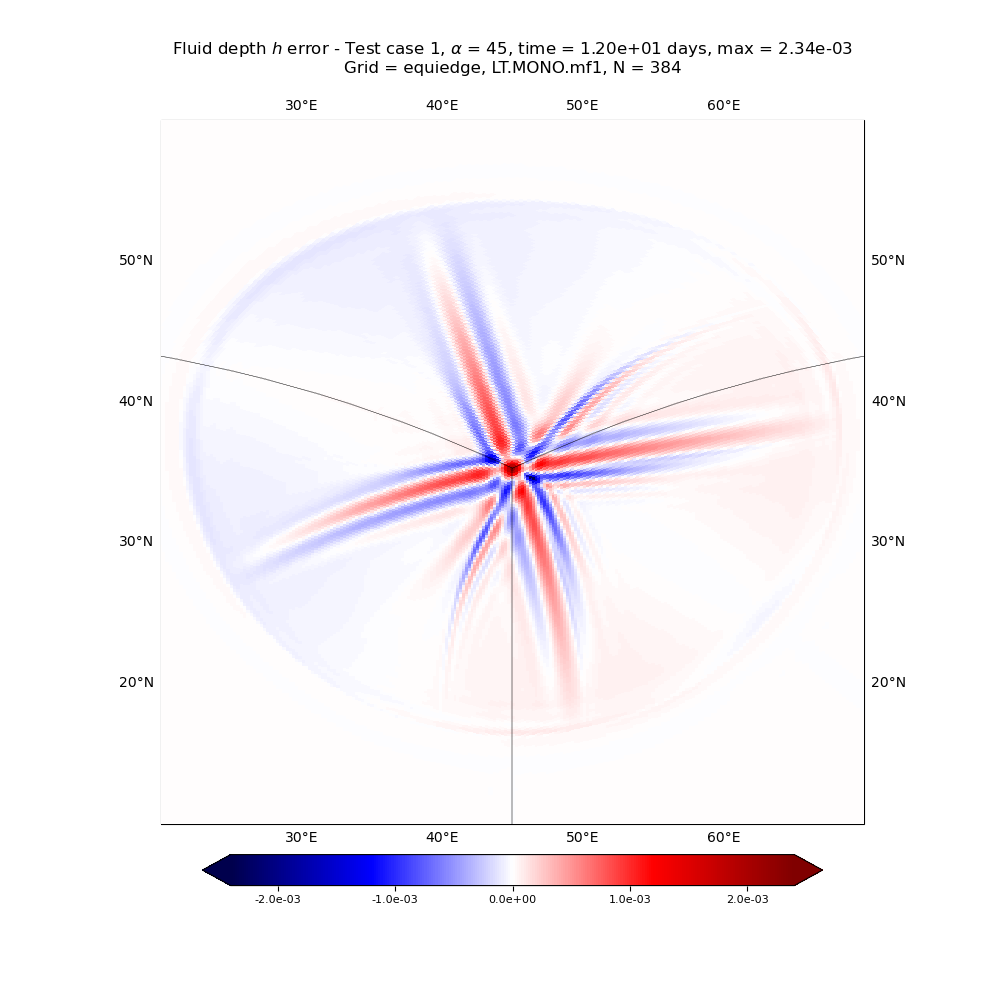
\includegraphics[width=1\linewidth]{h_error_tc1_t12_alpha45_C384_g0_dg2_adv2_hord8_mf1_tf12}
		\caption{LT scheme - max = $2.34\times 10^{-3}$\label{chp-advcs-sec-exp-adv5-errors-0b}}
	\end{subfigure}
	\caption{
		Advection experiment errors at a cube corner using the cosine bell (IC2, Table \ref{chp5-ic}) and  
the rotated zonal wind (VF1, Table \ref{chp5-vf}) after 12 days, using the monotonic scheme (MONO) 
		with PL (left) and LT schemes (right) on the equi-edge grid (g0) grid with $N=384$. 
		\label{chp-advcs-sec-exp-adv5-errors-0}}
\end{figure}
\begin{figure}[!htb]
	\centering
	\begin{subfigure}{0.35\textwidth}
		\centering
		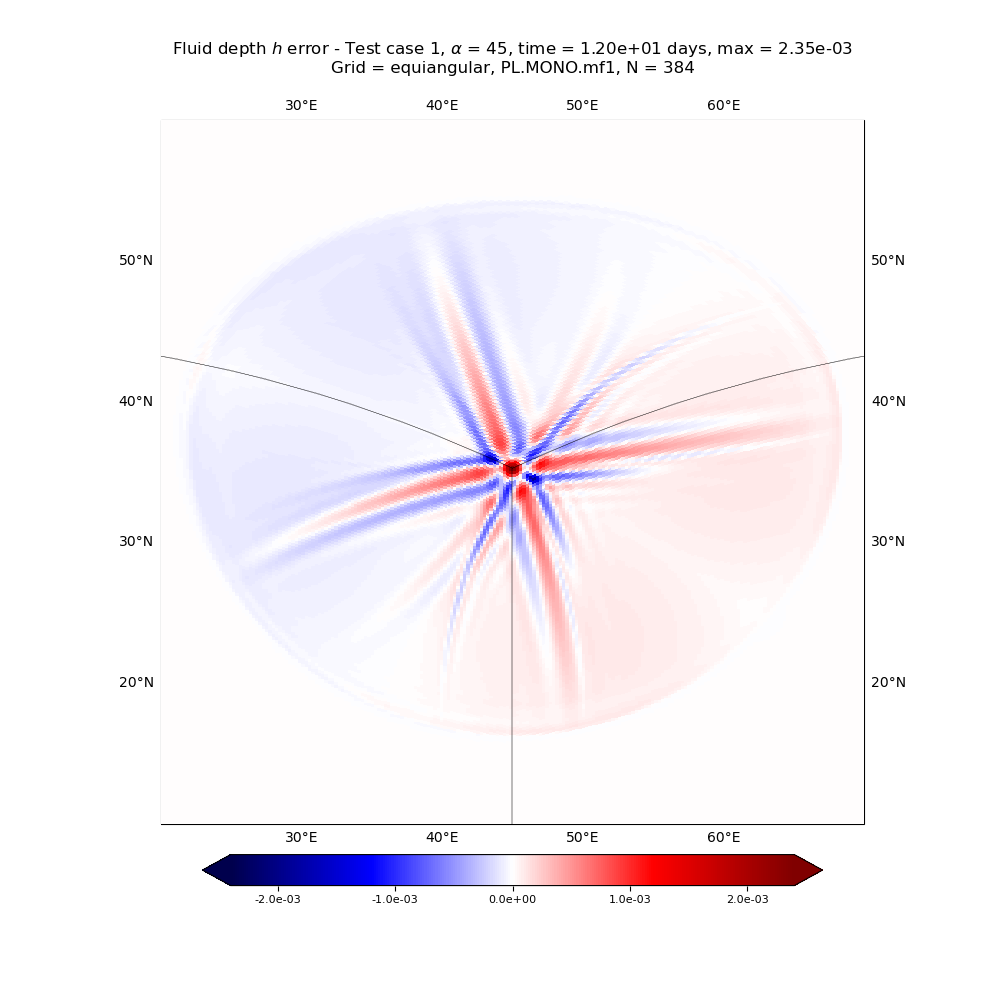
\includegraphics[width=1\linewidth]{h_error_tc1_t12_alpha45_C384_g2_dg2_adv1_hord8_mf1_tf12}
		\caption{PL scheme - max = $2.35\times 10^{-3}$\label{chp-advcs-sec-exp-adv5-errors-2a}}
	\end{subfigure}
	\begin{subfigure}{0.35\textwidth}
		\centering
		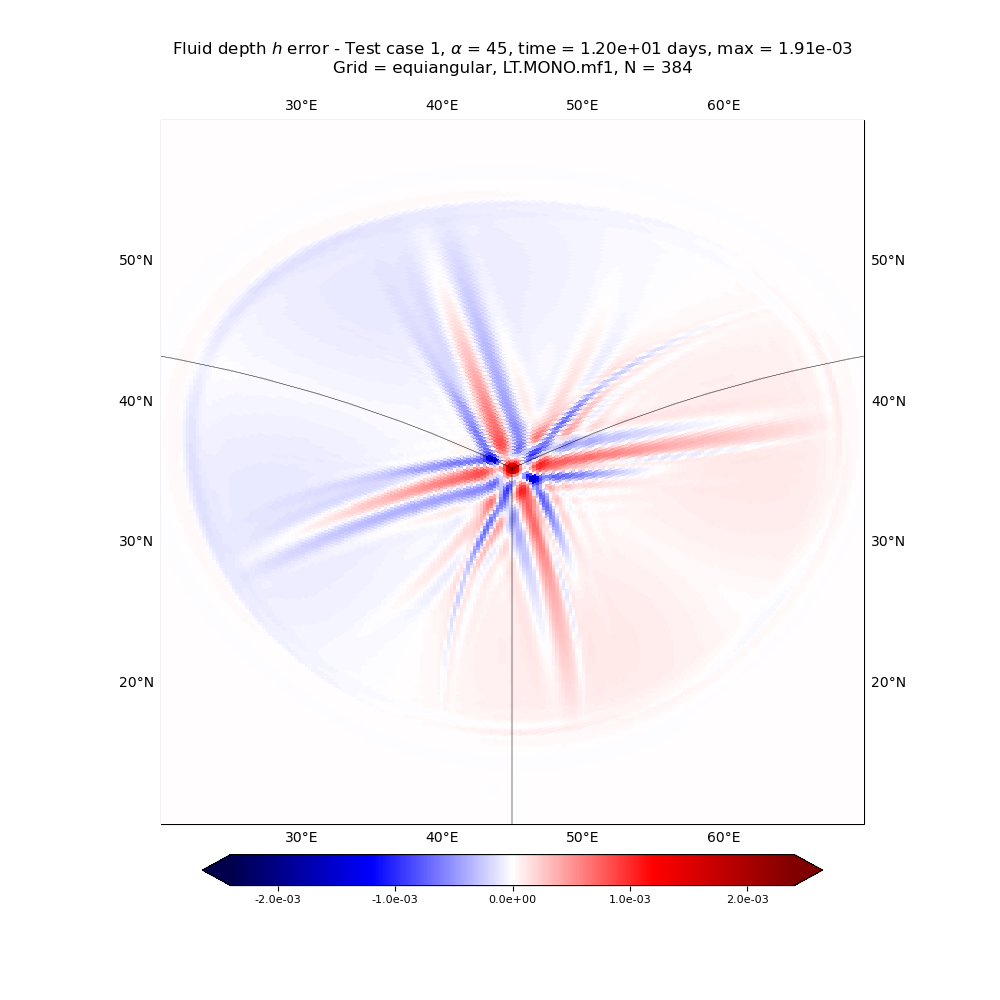
\includegraphics[width=1\linewidth]{h_error_tc1_t12_alpha45_C384_g2_dg2_adv2_hord8_mf1_tf12}
		\caption{LT scheme - max = $1.91\times 10^{-3}$ \label{chp-advcs-sec-exp-adv5-errors-2b}}
	\end{subfigure}
	\caption{As Figure \ref{chp-advcs-sec-exp-adv2-errors-0} but using the equiangular grid (g2).\label{chp-advcs-sec-exp-adv5-errors-2}}
\end{figure}

In Figure \ref{chp-advcs-sec-exp-adv5-errors-0}, we show the final error at the cube corner for the equi-edge grid (g0), 
and Figure \ref{chp-advcs-sec-exp-adv5-errors-2} show the same for the equiangular grid (g2).
We can observe that the results are similar to IC1 with VF1 shown in Figures \ref{chp-advcs-sec-exp-adv2-errors-0} and \ref{chp-advcs-sec-exp-adv2-errors-2}.
We conclude again that LT has a smaller error at the corner, especially for the equi-edge grid (g0).
\newpage
In Figures \ref{chp-advcs-sec-exp-adv5-linf} and \ref{chp-advcs-sec-exp-adv5-l2},
we show the error convergence for the $L_{\infty}$ and $L_2$ norms, respectively.
Note that the errors in the $L_{\infty}$ norm (Figure \ref{chp-advcs-sec-exp-adv5-linf})
for the unlimited PPM (solid lines) are not achieving second order as they should because the solution is not differentiable.
For MONO (dashed lines), we can see that the $L_{\infty}$ errors for LT (blue lines) are smaller than the errors of PL (green lines), 
especially for the equi-edge grid (g0).
%Also, for the equi-edge grid (g0), the order of the LT-MONO scheme in the $L_{\infty}$ norm gets very close to 2,
%and for the equiangular grid (g2), its order surpasses two.
%These results for LT-MONO are better than expected and are not observed for the PL-MONO scheme.
Finally, the $L_2$ errors are very similar (Figure \ref{chp-advcs-sec-exp-adv5-l2}).
\begin{figure}[!htb]
	\centering
	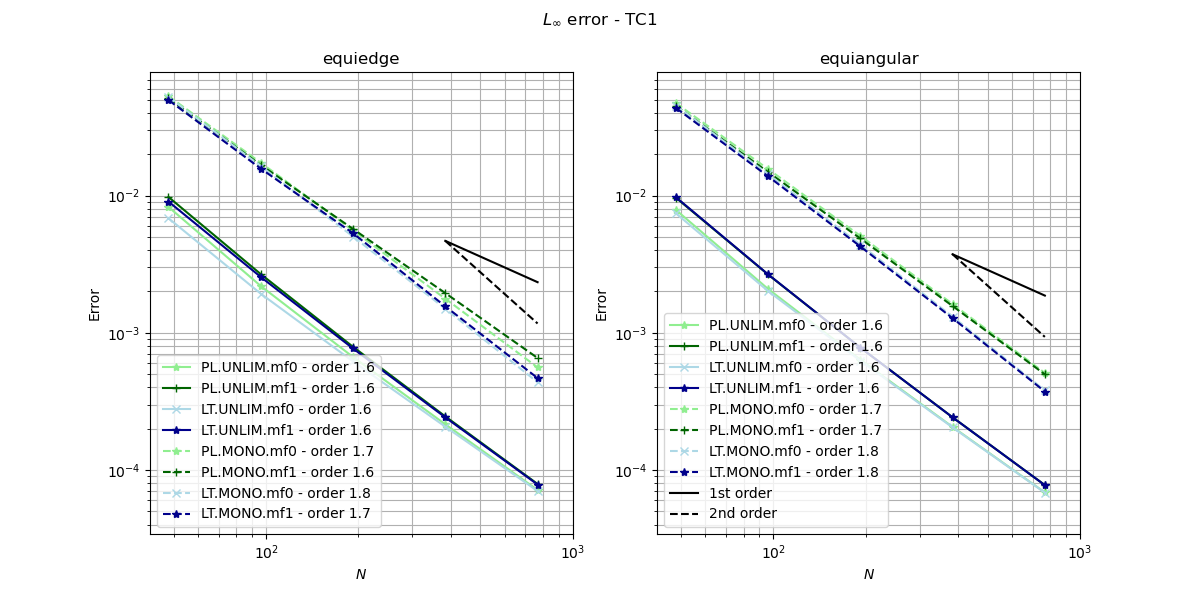
\includegraphics[width=0.8\linewidth]{linferror_tc1_alpha45}
	\caption{
		$L_{\infty}$ error convergence for the advection on the sphere test using the cosine bell at cube a corner (IC2, Table \ref{chp5-ic}) and 
		the rotated zonal wind  (VF1, Table \ref{chp5-vf}) on the equi-edge grid (g0, left) 
		and on the equiangular grid (g2, right) after 12 days.
		Blue lines indicate the use of the LT scheme, while green lines represent the PL scheme.
		Solid lines represent the results with the unlimited PPM (UNLIM) scheme, whereas dashed lines represent the results with monotonic (MONO).
		Light colors show the result without mass fixer (mf0), whereas dark colors show the results with flux averaging (mf1).
		\label{chp-advcs-sec-exp-adv5-linf}}
\end{figure}

\begin{figure}[!htb]
	\centering
	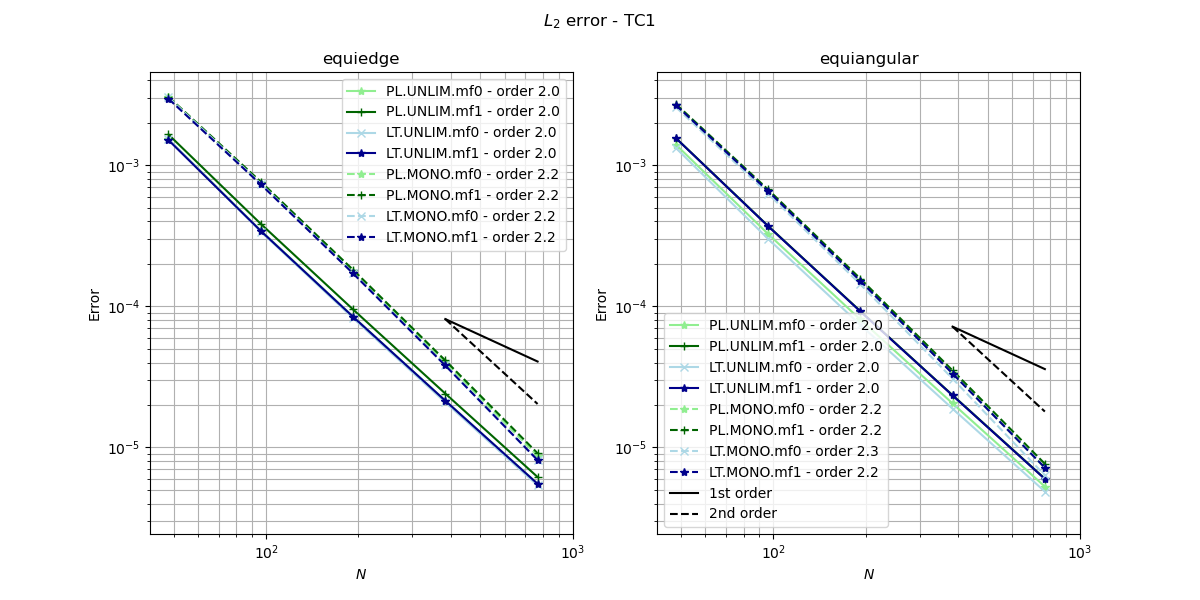
\includegraphics[width=0.8\linewidth]{l2error_tc1_alpha45}
	\caption{As Figure \ref{chp-advcs-sec-exp-adv3-linf} but considering the $L_2$ norm. \label{chp-advcs-sec-exp-adv5-l2}}
\end{figure}

\newpage
\subsection{Advection of a slotted cylinder through the rotated zonal wind}
The third test case here is the slotted cylinder advection, given by IC3 from Table \ref{chp5-ic} and using again the rotated zonal wind VF1 (Table \ref{chp5-vf}).
We show how the solution evolves with time in Figure \ref{chp-advcs-sec-exp-adv6}.

\begin{figure}[!htb]
	\centering
	\begin{subfigure}{0.45\textwidth}
		\centering
		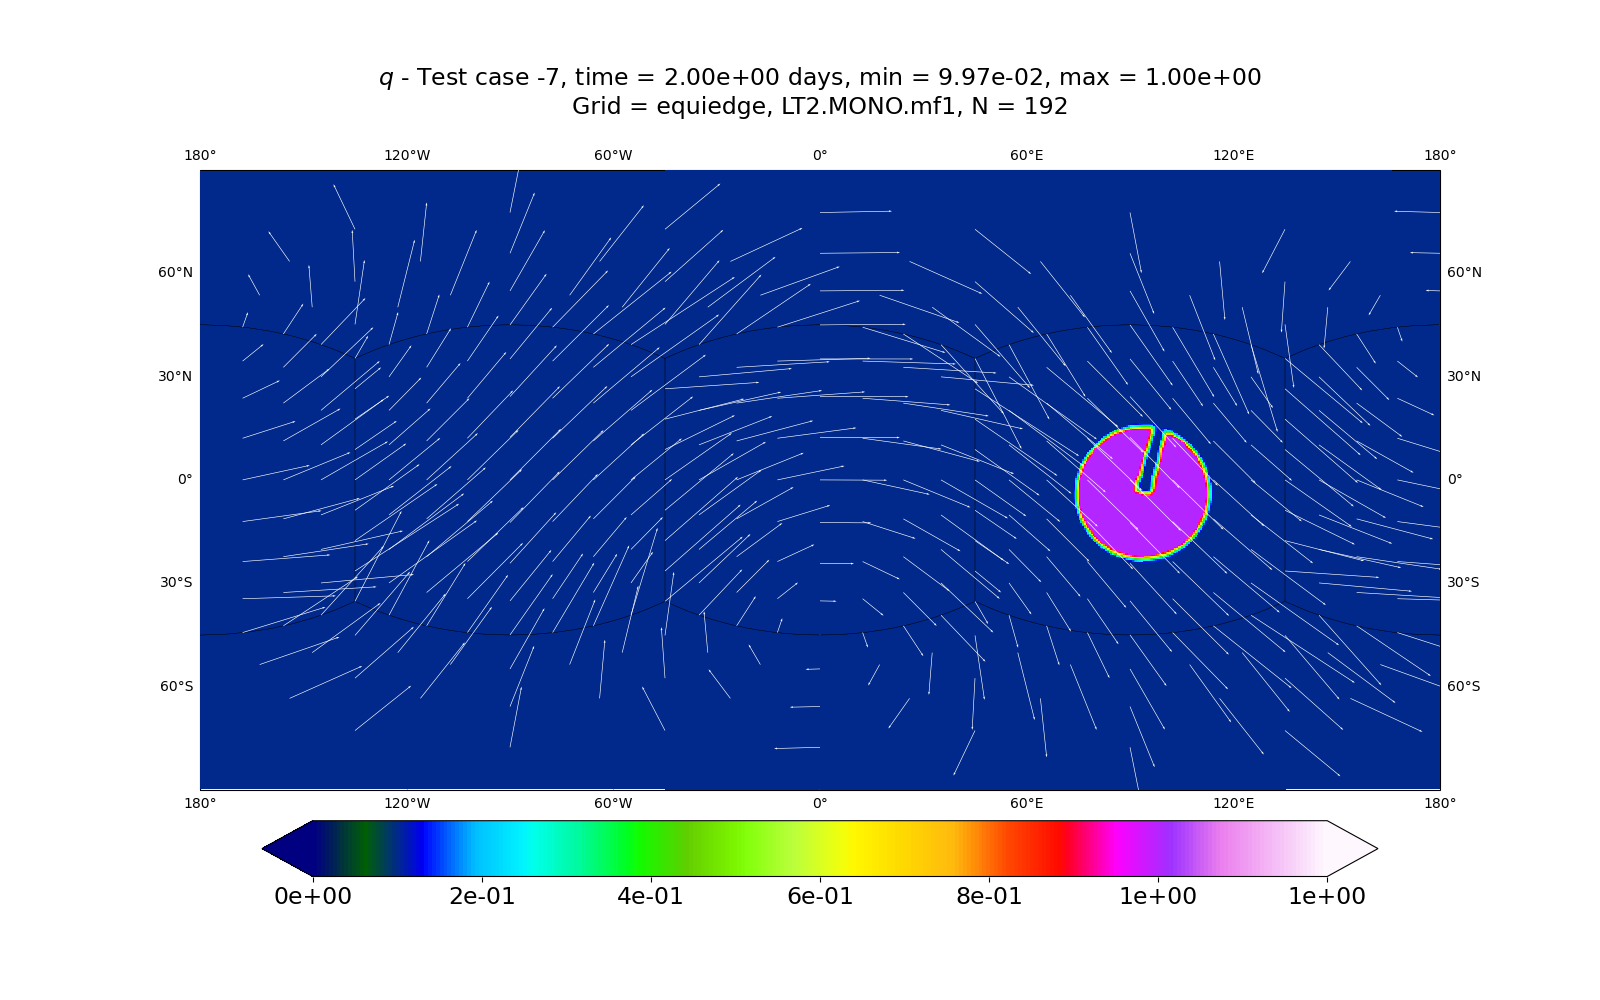
\includegraphics[width=1\linewidth]{h_tc-7_t2_alpha45_C192_g0_dg2_adv2_hord8_mf1_tf12}
		\caption{$t=2$ days.\label{chp-advcs-sec-exp-adv6-a}}
	\end{subfigure}
	\begin{subfigure}{0.45\textwidth}
		\centering
		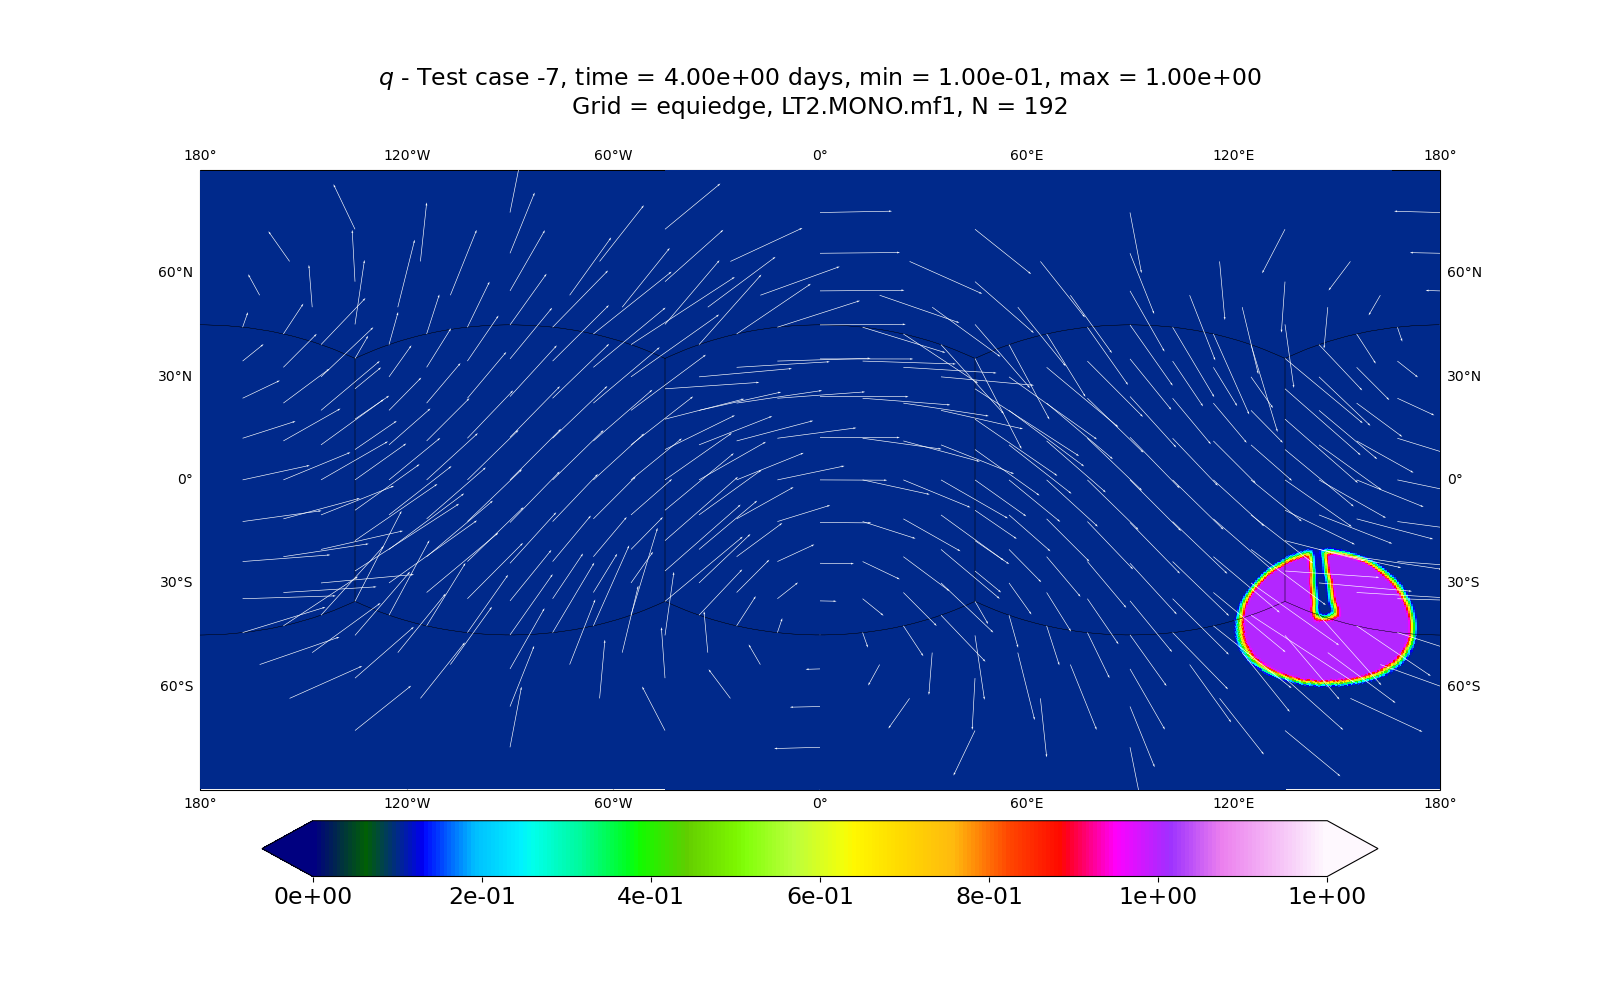
\includegraphics[width=1\linewidth]{h_tc-7_t4_alpha45_C192_g0_dg2_adv2_hord8_mf1_tf12}
		\caption{$t=4$ days.\label{chp-advcs-sec-exp-adv6-b}}
	\end{subfigure}
	
	\begin{subfigure}{0.45\textwidth}
		\centering
		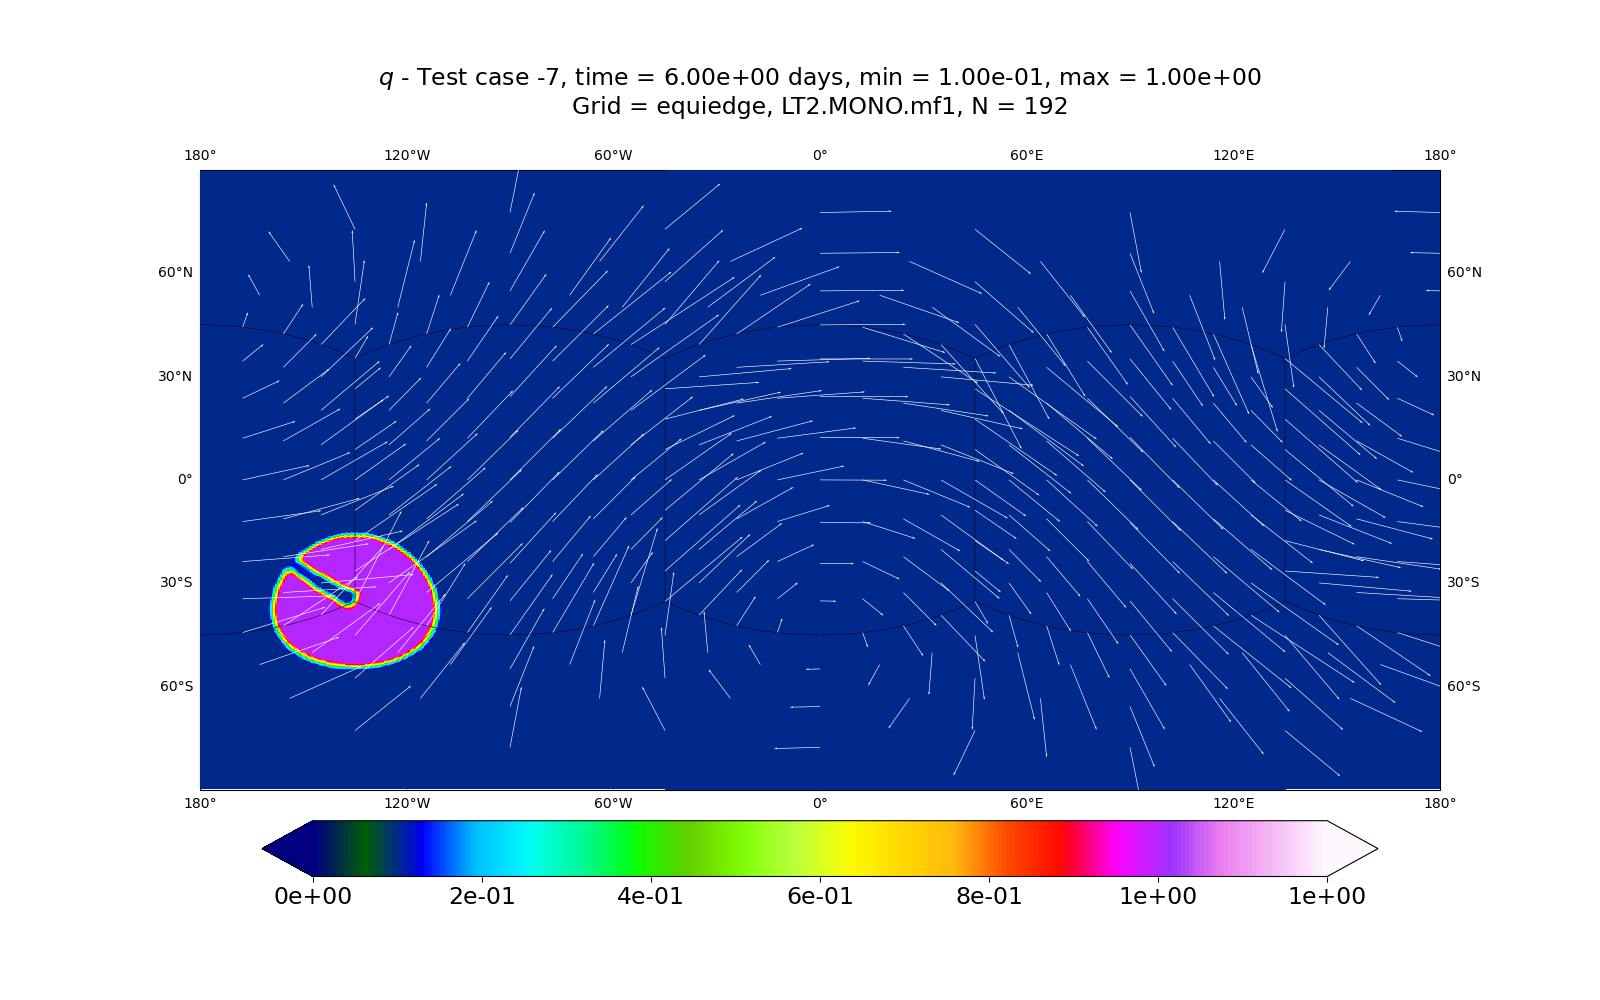
\includegraphics[width=1\linewidth]{h_tc-7_t6_alpha45_C192_g0_dg2_adv2_hord8_mf1_tf12}
		\caption{$t=6$ days.\label{chp-advcs-sec-exp-adv6-c}}
	\end{subfigure}	
	\begin{subfigure}{0.45\textwidth}
		\centering
		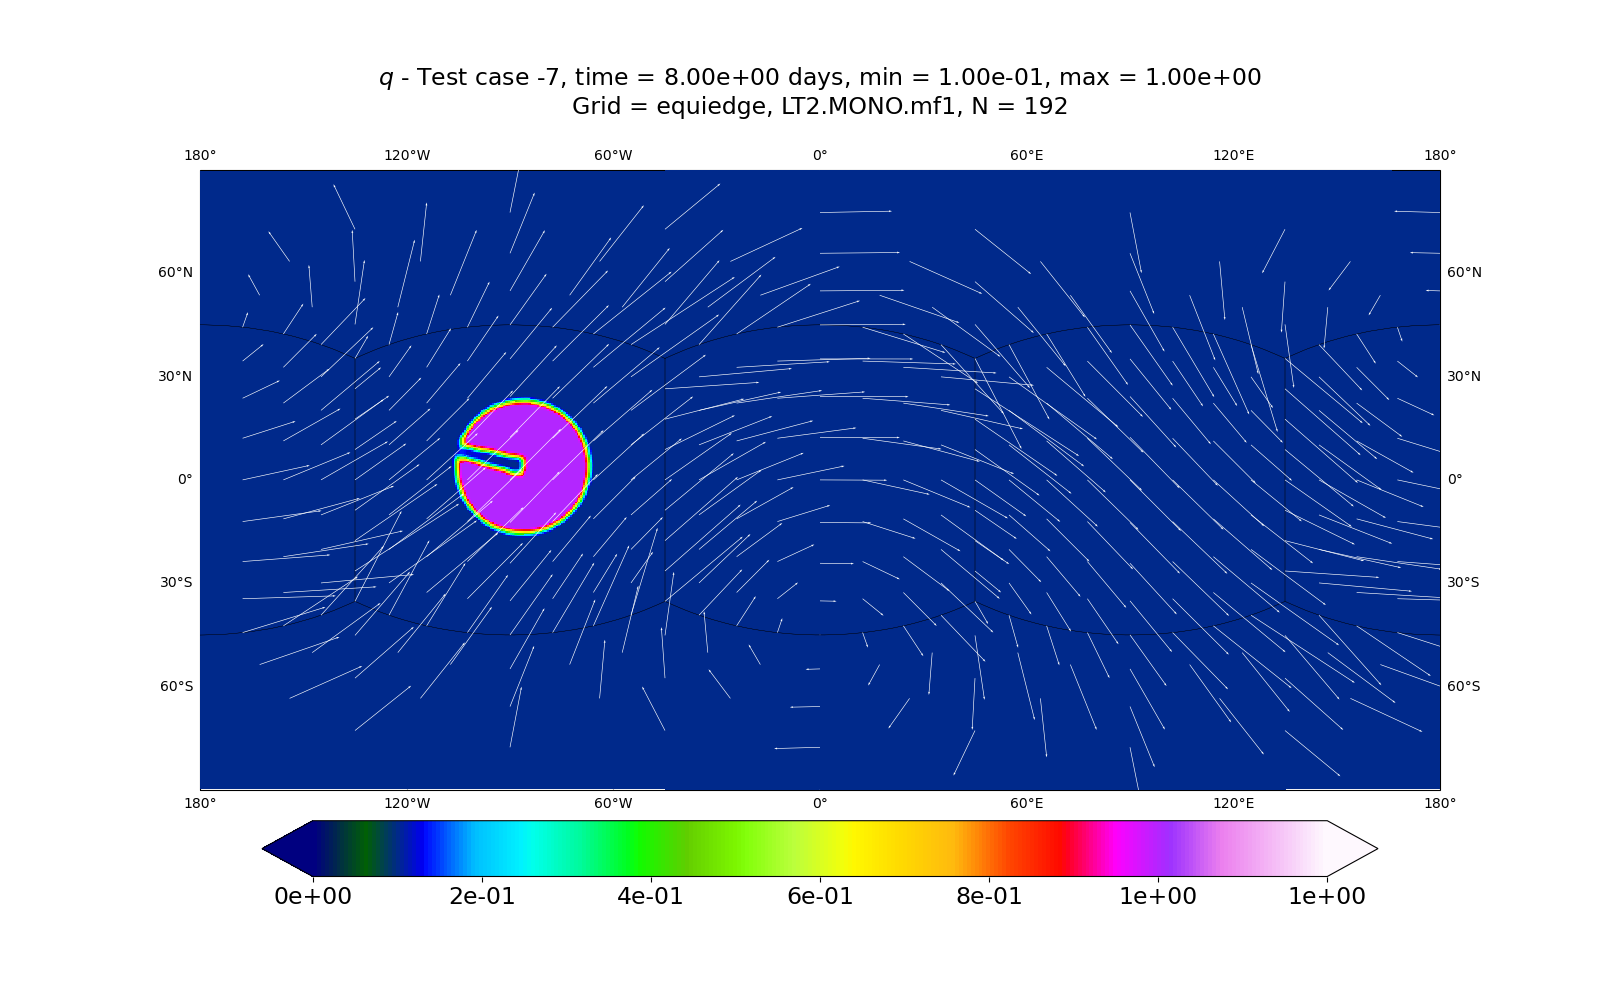
\includegraphics[width=1\linewidth]{h_tc-7_t8_alpha45_C192_g0_dg2_adv2_hord8_mf1_tf12}
		\caption{$t=8$ days.\label{chp-advcs-sec-exp-adv6-d}}
	\end{subfigure}
	
	\begin{subfigure}{0.45\textwidth}
		\centering
		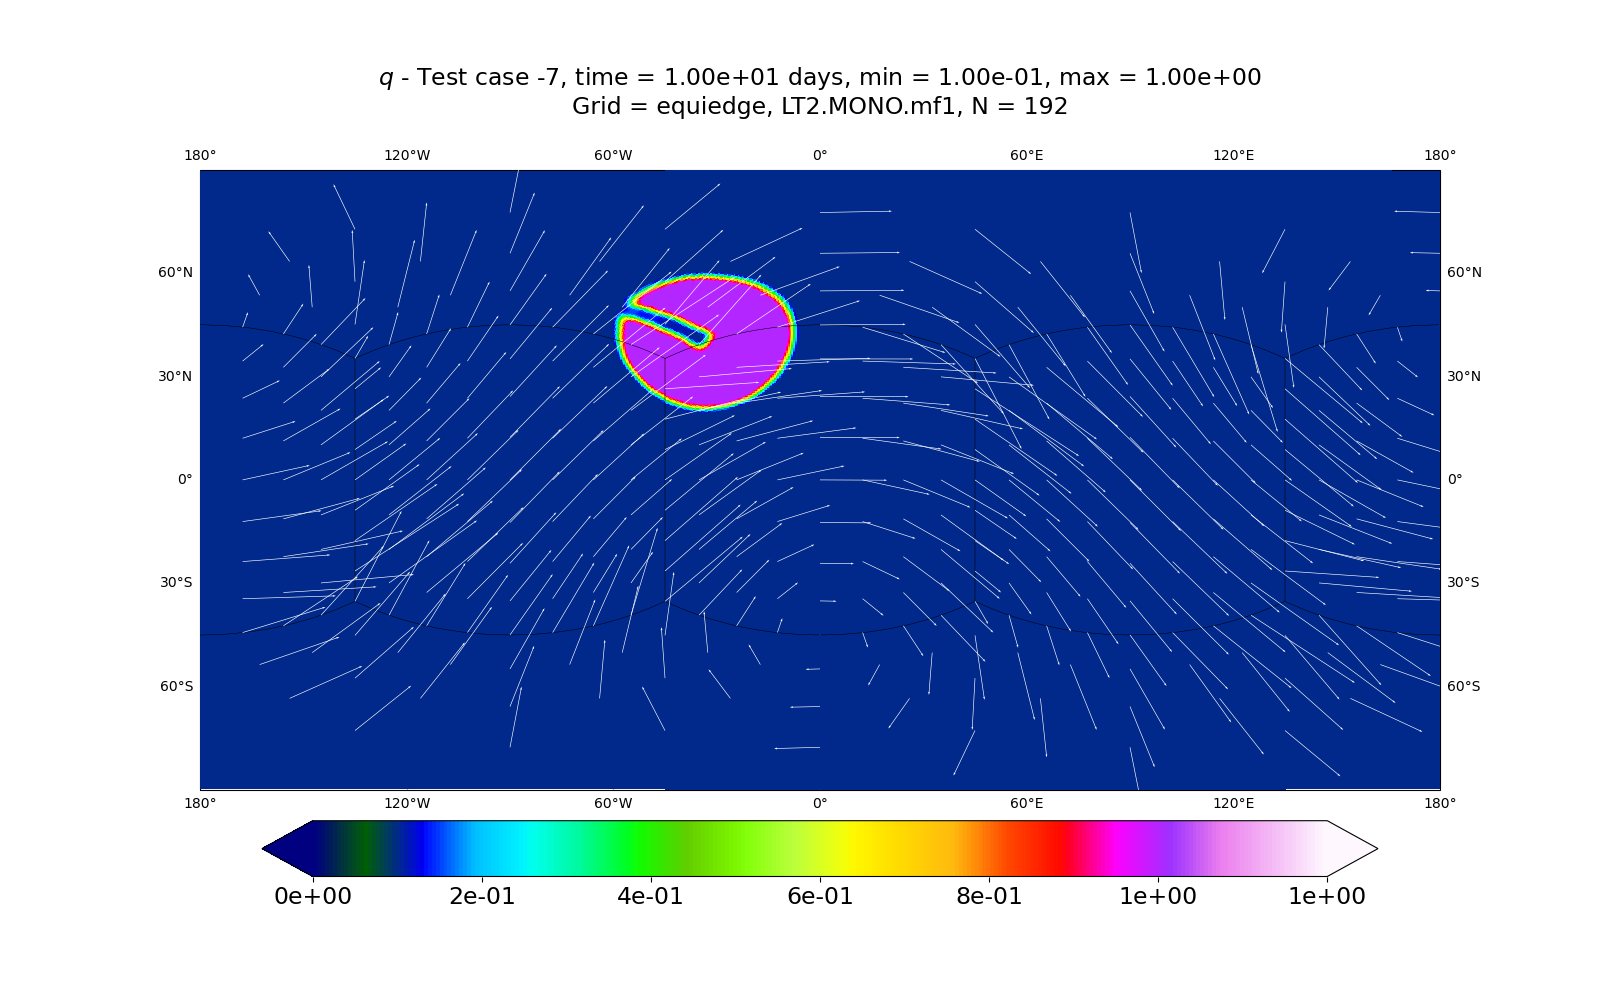
\includegraphics[width=1\linewidth]{h_tc-7_t10_alpha45_C192_g0_dg2_adv2_hord8_mf1_tf12}
		\caption{$t=10$ days.\label{chp-advcs-sec-exp-adv6-e}}
	\end{subfigure}
	\begin{subfigure}{0.45\textwidth}
		\centering
		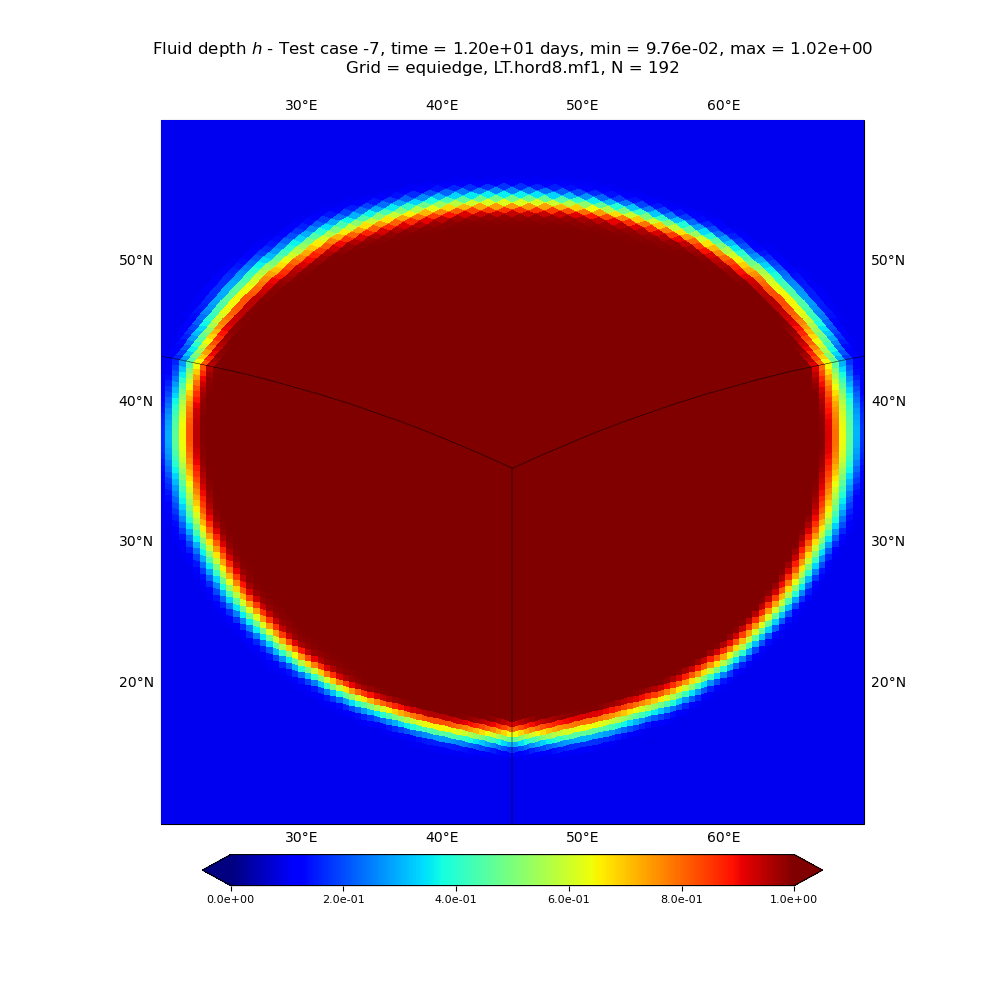
\includegraphics[width=1\linewidth]{h_tc-7_t12_alpha45_C192_g0_dg2_adv2_hord8_mf1_tf12}
		\caption{$t=12$ days.\label{chp-advcs-sec-exp-adv6-f}}
	\end{subfigure}
	\caption{Advection experiment results using the slotted cylinder at a cube corner (IC3, Table \ref{chp5-ic}) and 
		the rotated zonal wind (VF1, Table \ref{chp5-vf}).
		These figures show the advected profile after
		2 \eqref{chp-advcs-sec-exp-adv6-a}, 
		4  \eqref{chp-advcs-sec-exp-adv6-b},
		6  \eqref{chp-advcs-sec-exp-adv6-c},
		8  \eqref{chp-advcs-sec-exp-adv6-d},
		10  \eqref{chp-advcs-sec-exp-adv6-e},
		and 12  \eqref{chp-advcs-sec-exp-adv6-f} days.
		We are using the LT-MONO-mf1 scheme on the equi-edge grid (g2) with $N=192$. \label{chp-advcs-sec-exp-adv6}}
\end{figure}

The goal of this test is to assess the qualitative behavior of the solution, 
especially to see if the limiter prevents oscillations that are expected since the slotted cylinder has a discontinuous profile.
Also, as the slotted cylinder is located at a cube corner, we would like to see if the corner affects the solution.
In Figure \ref{chp-advcs-sec-exp-adv7}, we present the final solutions for $N=192$ as well the reference solution.
It is evident that all the schemes yield similar results, and we cannot observe any interference of the corner despite using a discontinuous initial condition.

\begin{figure}[!htb]
	\centering
	\begin{subfigure}{0.3\textwidth}
		\centering
		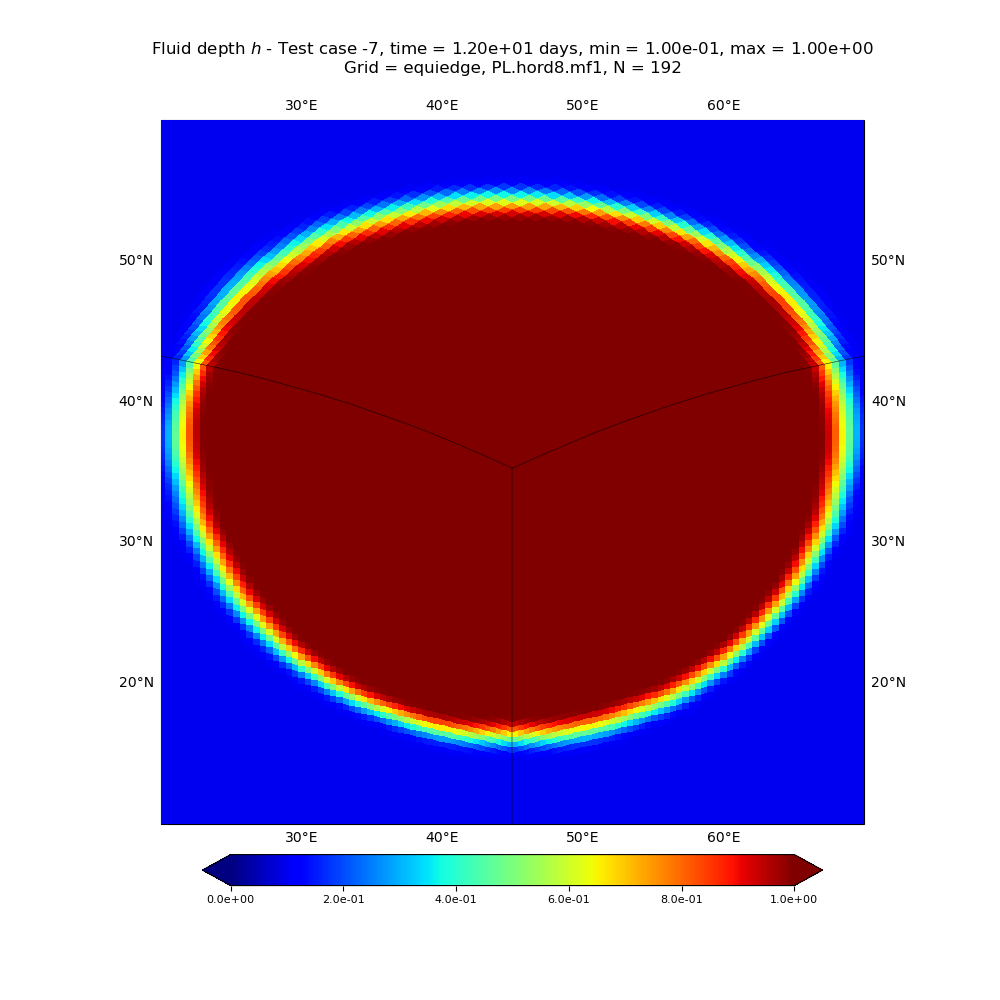
\includegraphics[width=1\linewidth]{h_tc-7_t12_alpha45_C192_g0_dg2_adv1_hord8_mf1_tf12}
		\caption{PL-MONO at g0.\label{chp-advcs-sec-exp-adv7-b}}
	\end{subfigure}
	\begin{subfigure}{0.3\textwidth}
		\centering
		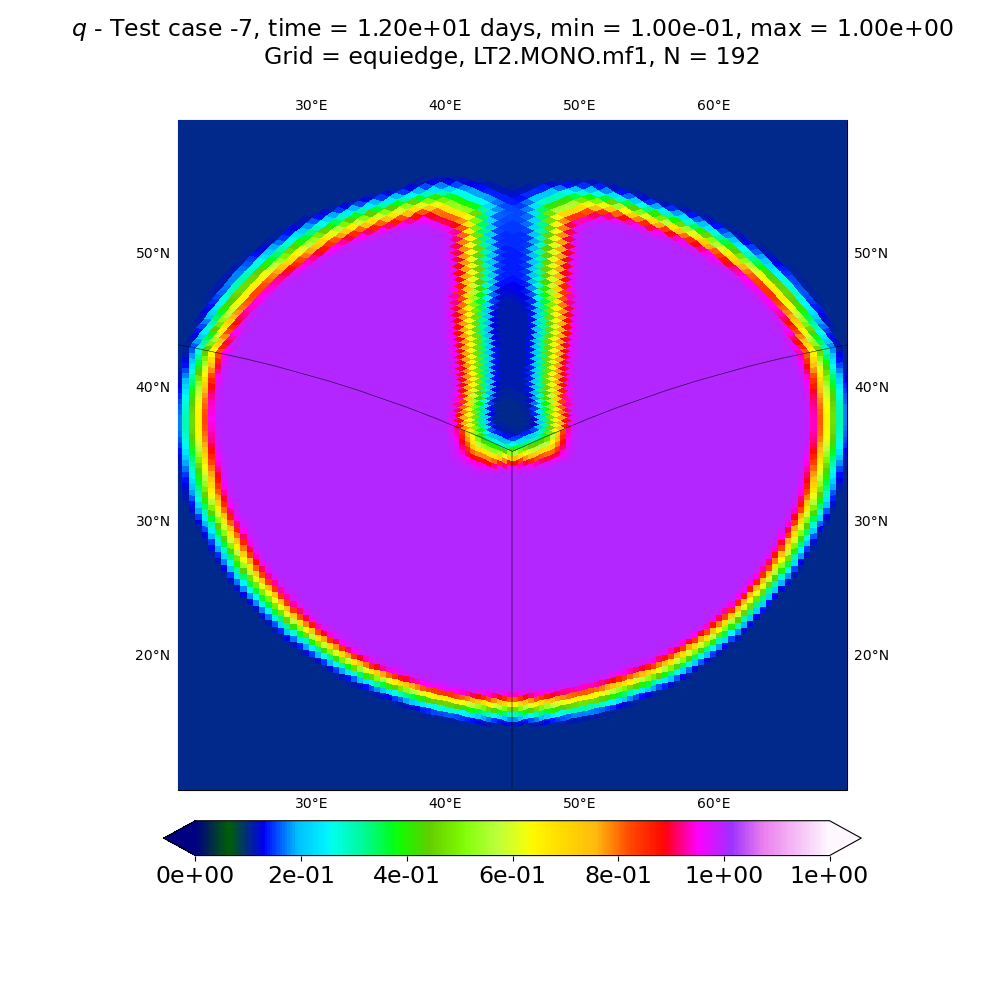
\includegraphics[width=1\linewidth]{h_tc-7_t12_alpha45_C192_g0_dg2_adv2_hord8_mf1_tf12a}
		\caption{LT-MONO at g0.\label{chp-advcs-sec-exp-adv7-c}}
	\end{subfigure}
	
	\begin{subfigure}{0.3\textwidth}
		\centering
		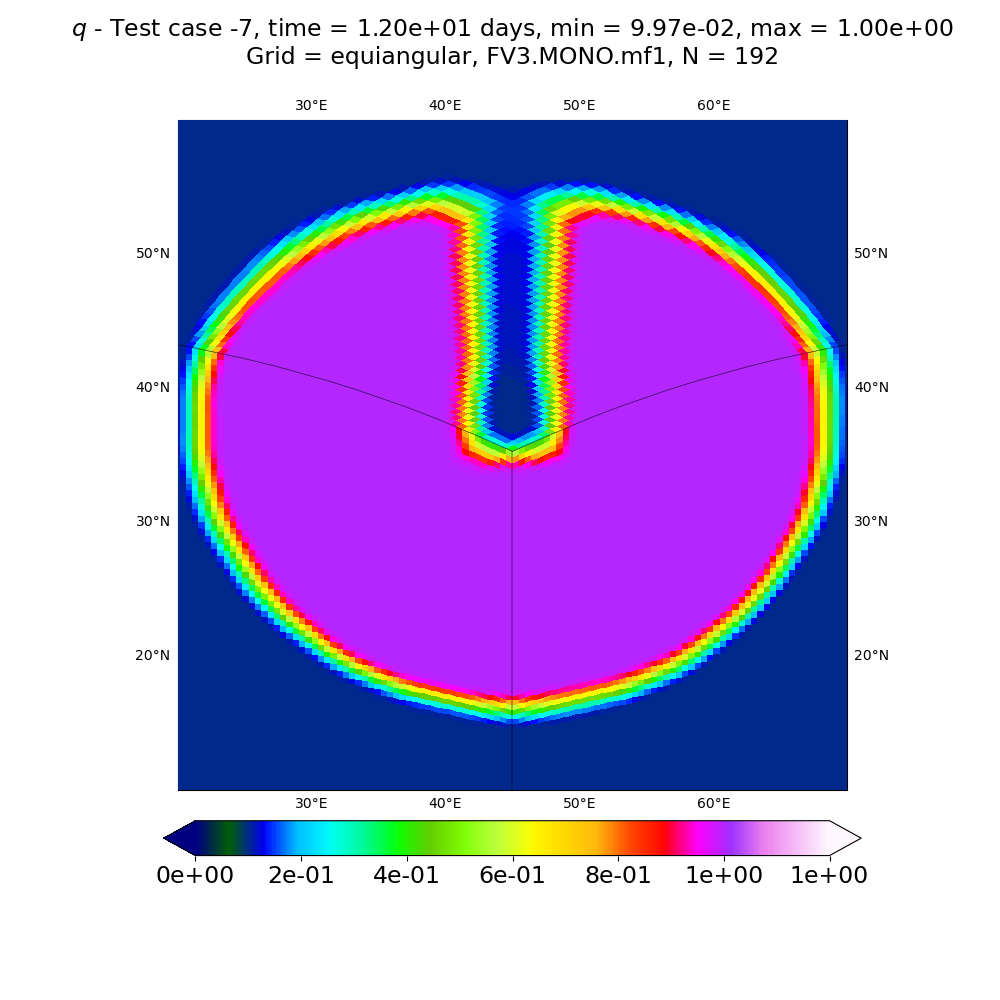
\includegraphics[width=1\linewidth]{h_tc-7_t12_alpha45_C192_g2_dg2_adv1_hord8_mf1_tf12}
		\caption{PL-MONO at g2.\label{chp-advcs-sec-exp-adv7-d}}
	\end{subfigure}
	\begin{subfigure}{0.3\textwidth}
	\centering
	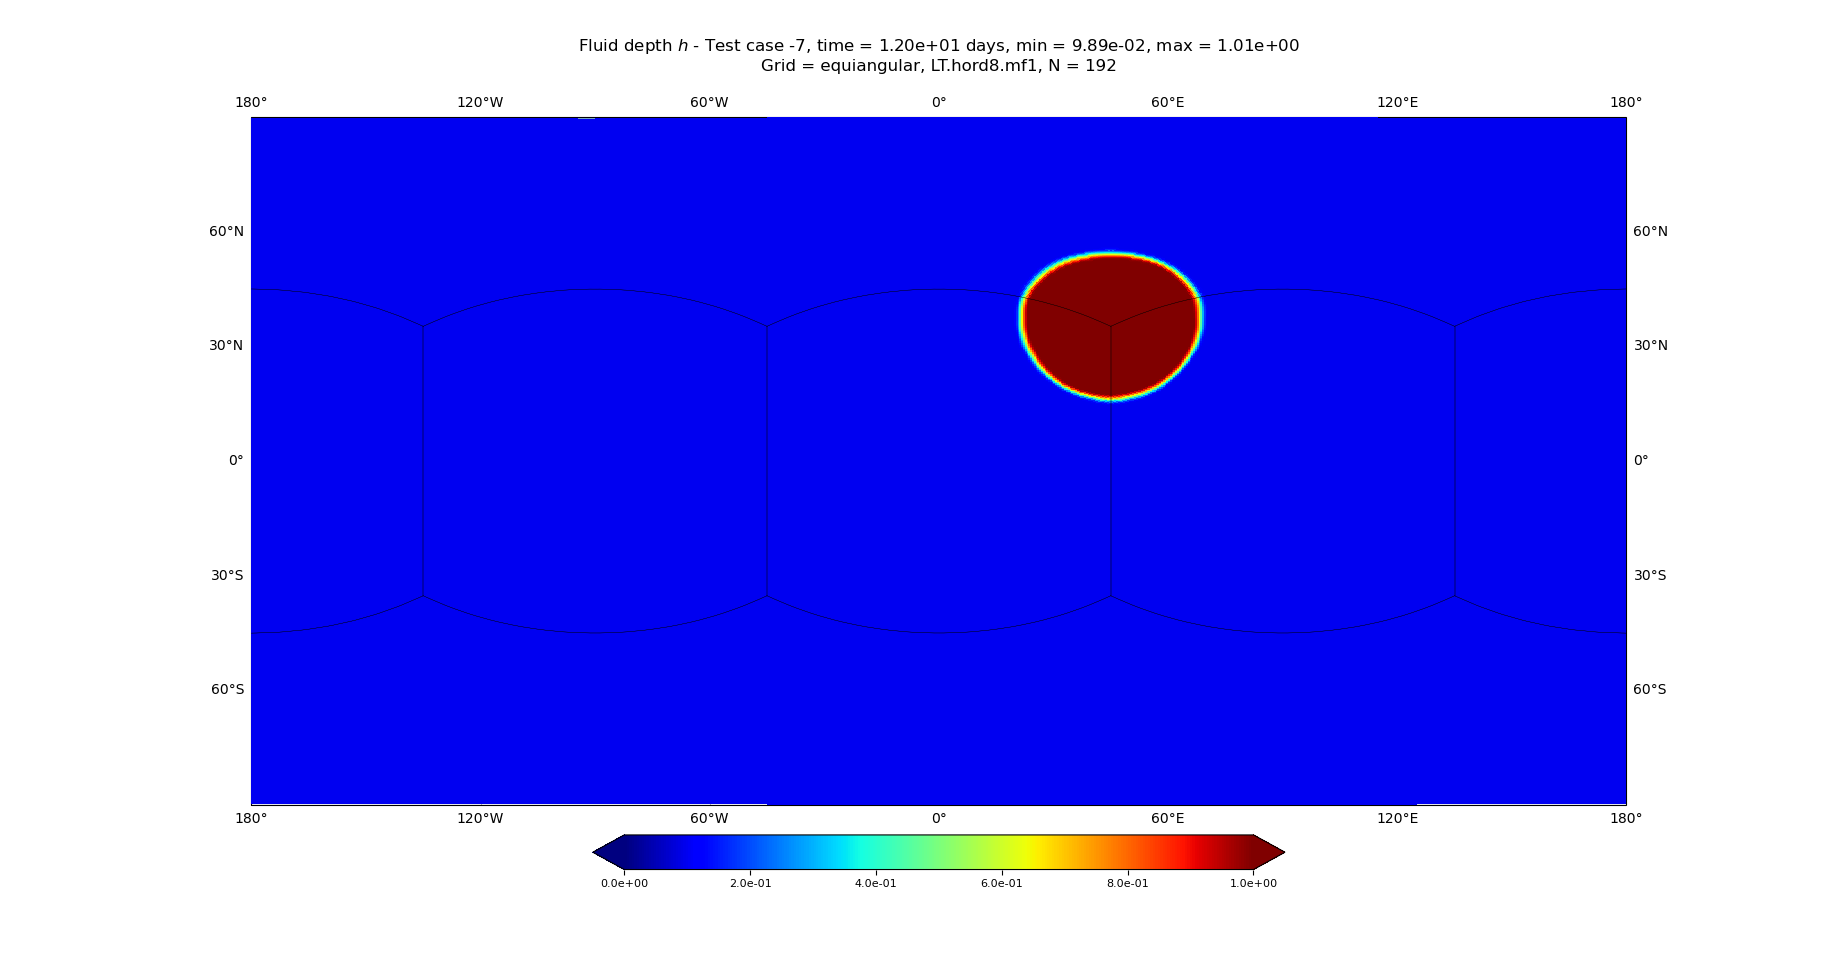
\includegraphics[width=1\linewidth]{h_tc-7_t12_alpha45_C192_g2_dg2_adv2_hord8_mf1_tf12}
	\caption{LT-MONO at g2.\label{chp-advcs-sec-exp-adv7-e}}
    \end{subfigure}

	\begin{subfigure}{0.3\textwidth}
	\centering
	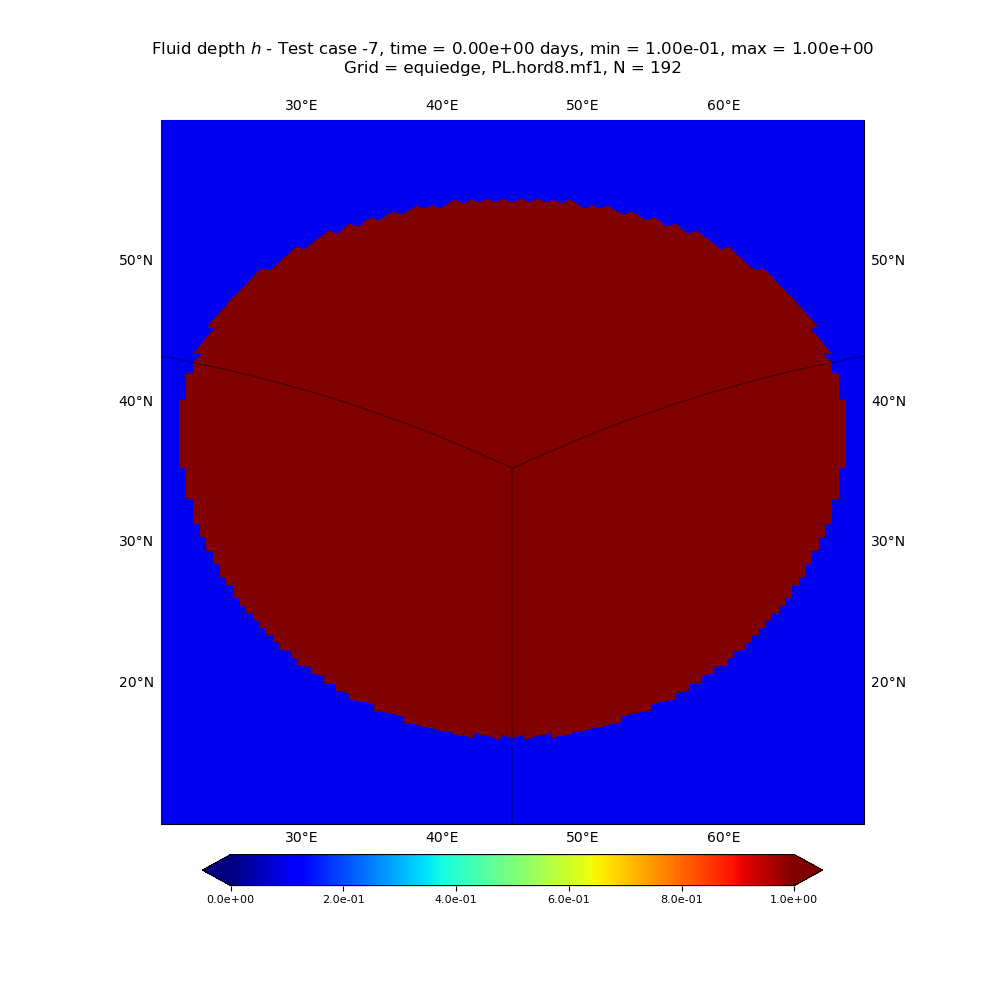
\includegraphics[width=1\linewidth]{h_tc-7_t0_alpha45_C192_g0_dg2_adv1_hord8_mf1_tf12}
	\caption{IC and exact solution at day 12.\label{chp-advcs-sec-exp-adv7-a}}
    \end{subfigure}
	\caption{Slotted cylinder at corner test with $N=192$ after 12 days for the schemes 
	PL-MONO at the equi-edge grid (g0) (a),	LT-MONO at the equi-edge grid (g0) (b), 
	PL-MONO at the equiangular grid (g2) (c) and LT-MONO at the equiangular grid (g2) (d).
	(e) depicts the reference solution. The monotonic scheme is denoted by MONO.
	\label{chp-advcs-sec-exp-adv7}}
\end{figure}

\newpage
\subsection{Non-divergent deformational flow}
The fourth test case considers the divergence free wind VF2 from Table \ref{chp5-vf}, along with the initial condition IC4 from Table \ref{chp5-tab1}, 
where the velocity is time-dependent.
This test is suggested by \citet{nair:2010}, and Figure \ref{chp-advcs-sec-exp-adv3} shows how the solution evolves over time.
Since the wind is divergence free, we observe that it deforms the two Gaussian hills, without creating new extrema.
Eventually, the final solution is equal to the initial condition after 12 days.
This test is the spherical analogous of the planar divergence free deformational flow test presented in Section \ref{2d-adv-ndivflow}.
\begin{figure}[!htb]
	\centering
	\begin{subfigure}{0.45\textwidth}
		\centering
		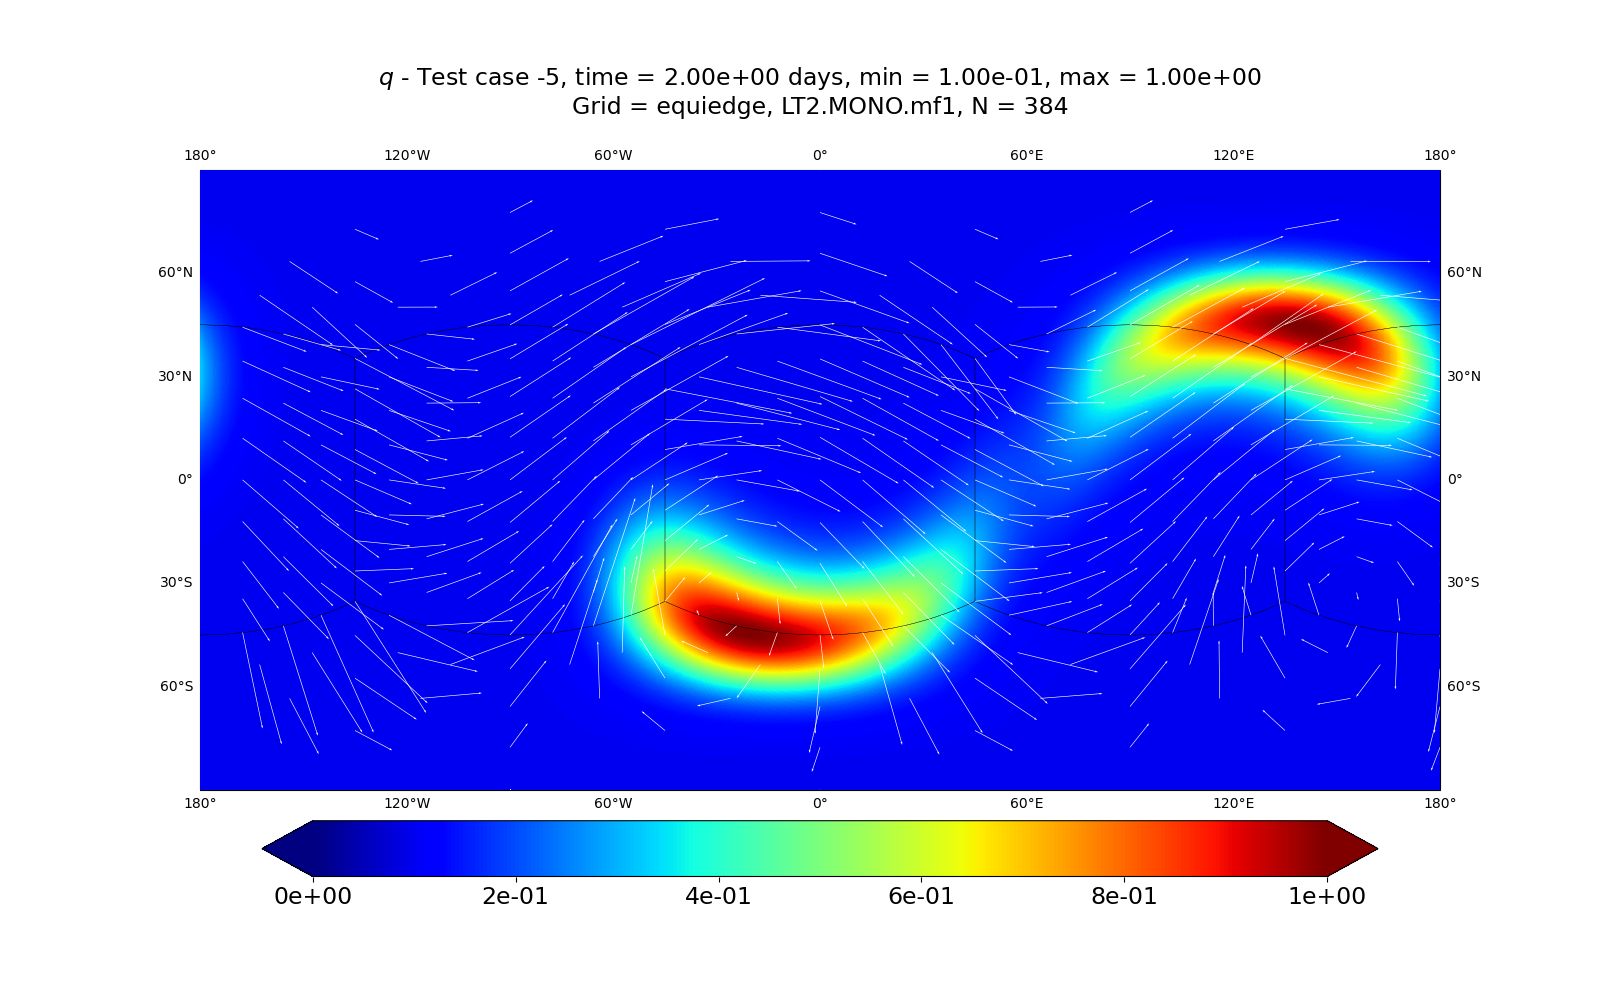
\includegraphics[width=1\linewidth]{h_tc-5_t2_alpha0_C384_g0_dg2_adv2_hord8_mf1_tf12}
		\caption{$t=2$ days.\label{chp-advcs-sec-exp-adv3-a}}
	\end{subfigure}
	\begin{subfigure}{0.45\textwidth}
		\centering
		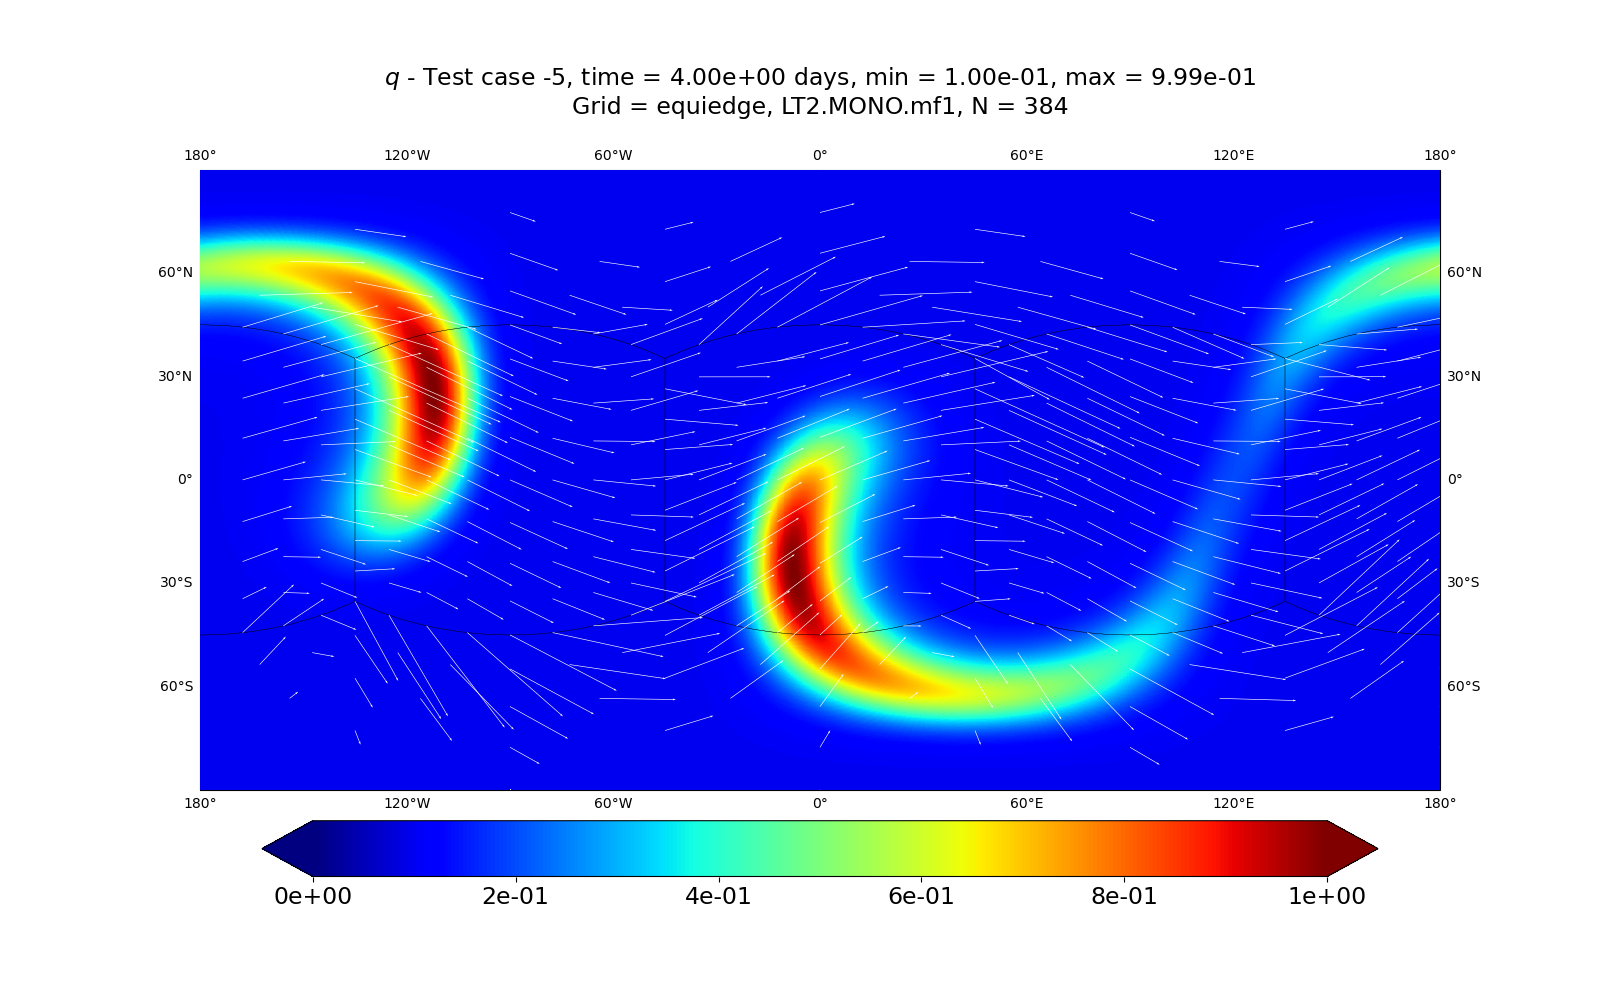
\includegraphics[width=1\linewidth]{h_tc-5_t4_alpha0_C384_g0_dg2_adv2_hord8_mf1_tf12}
		\caption{$t=4$ days.\label{chp-advcs-sec-exp-adv3-b}}
	\end{subfigure}

	\begin{subfigure}{0.45\textwidth}
		\centering
		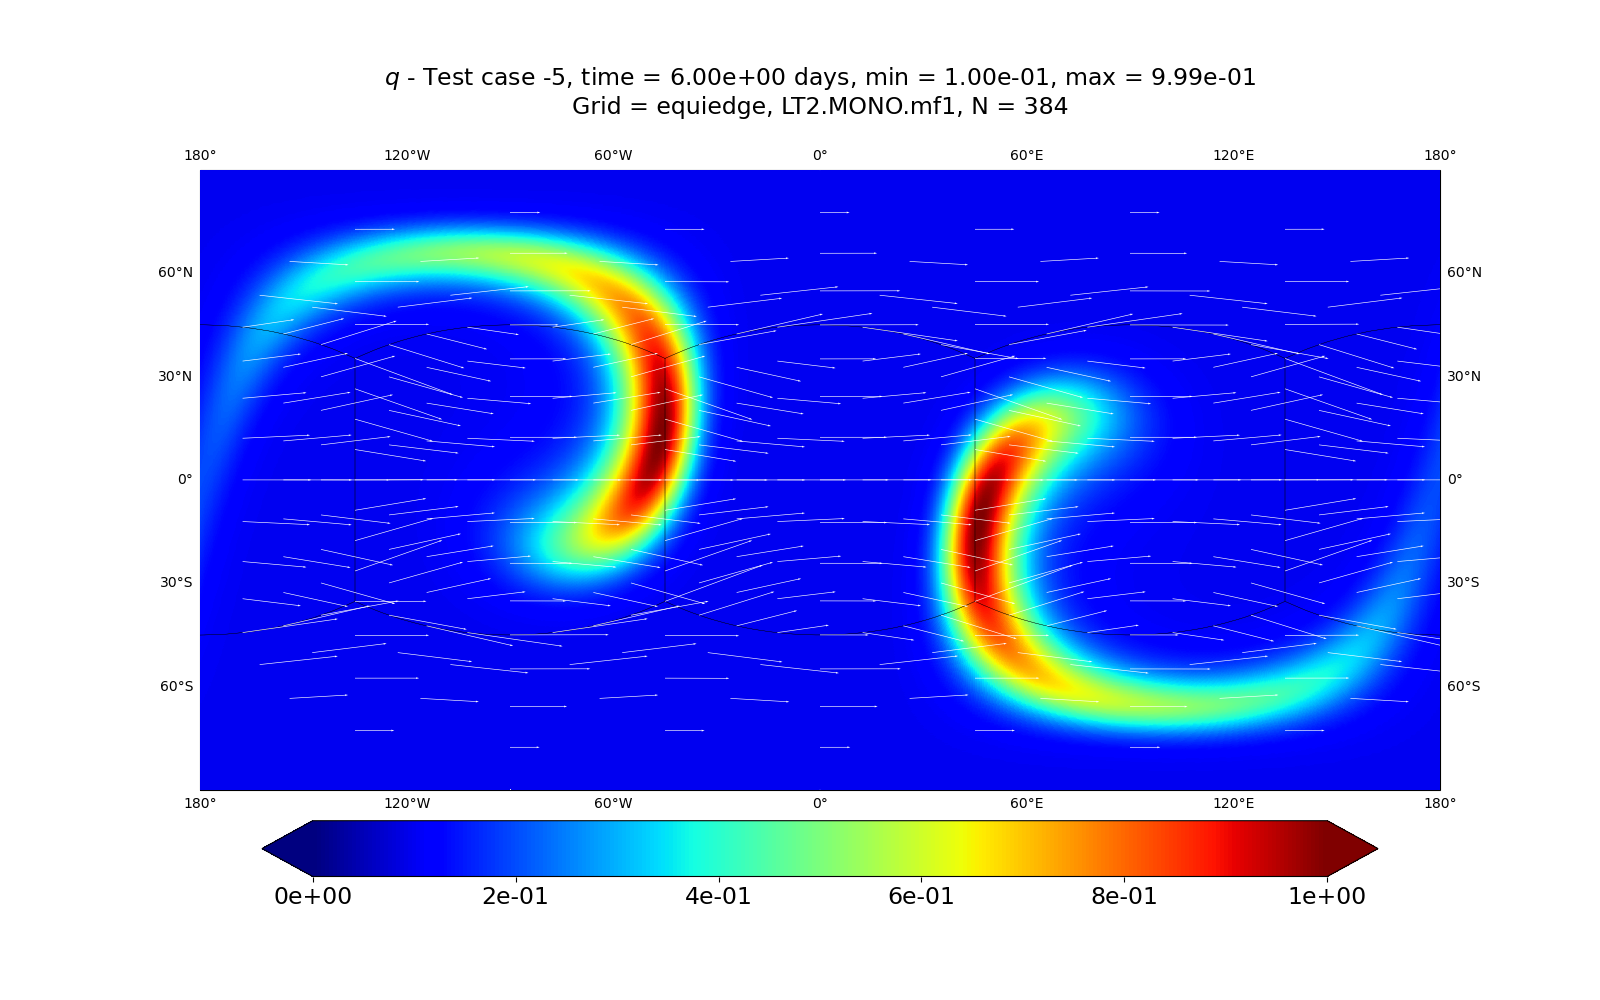
\includegraphics[width=1\linewidth]{h_tc-5_t6_alpha0_C384_g0_dg2_adv2_hord8_mf1_tf12}
		\caption{$t=6$ days.\label{chp-advcs-sec-exp-adv3-c}}
	\end{subfigure}
	\begin{subfigure}{0.45\textwidth}
		\centering
		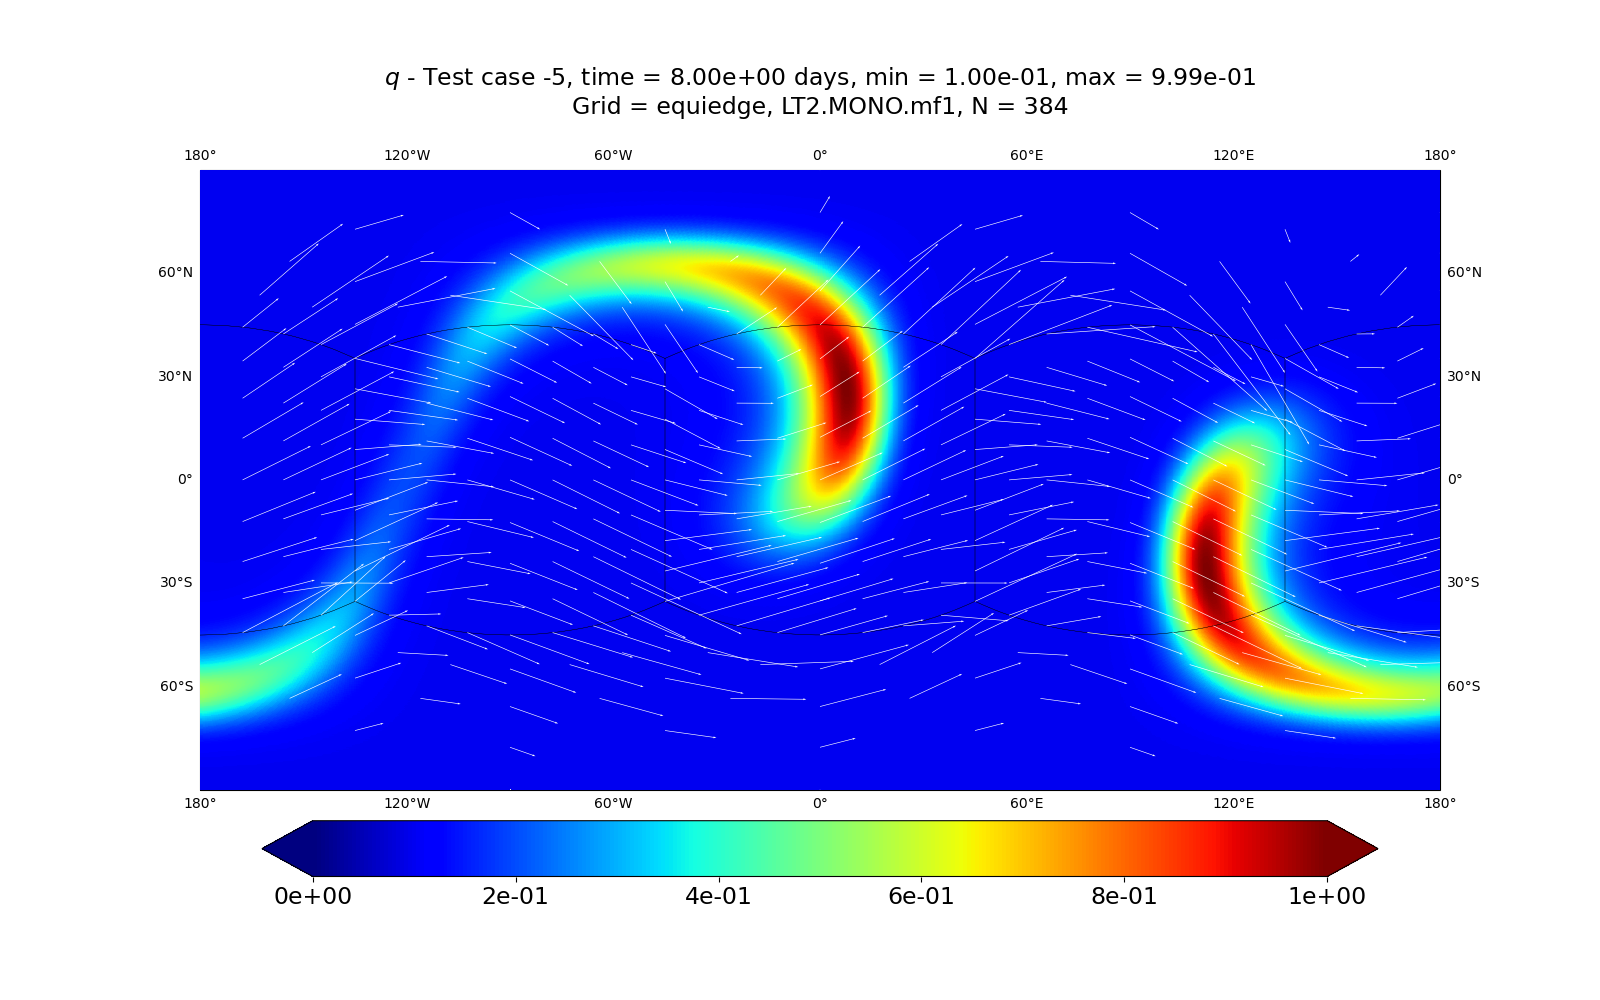
\includegraphics[width=1\linewidth]{h_tc-5_t8_alpha0_C384_g0_dg2_adv2_hord8_mf1_tf12}
		\caption{$t=8$ days.\label{chp-advcs-sec-exp-adv3-d}}
	\end{subfigure}

	\begin{subfigure}{0.45\textwidth}
		\centering
		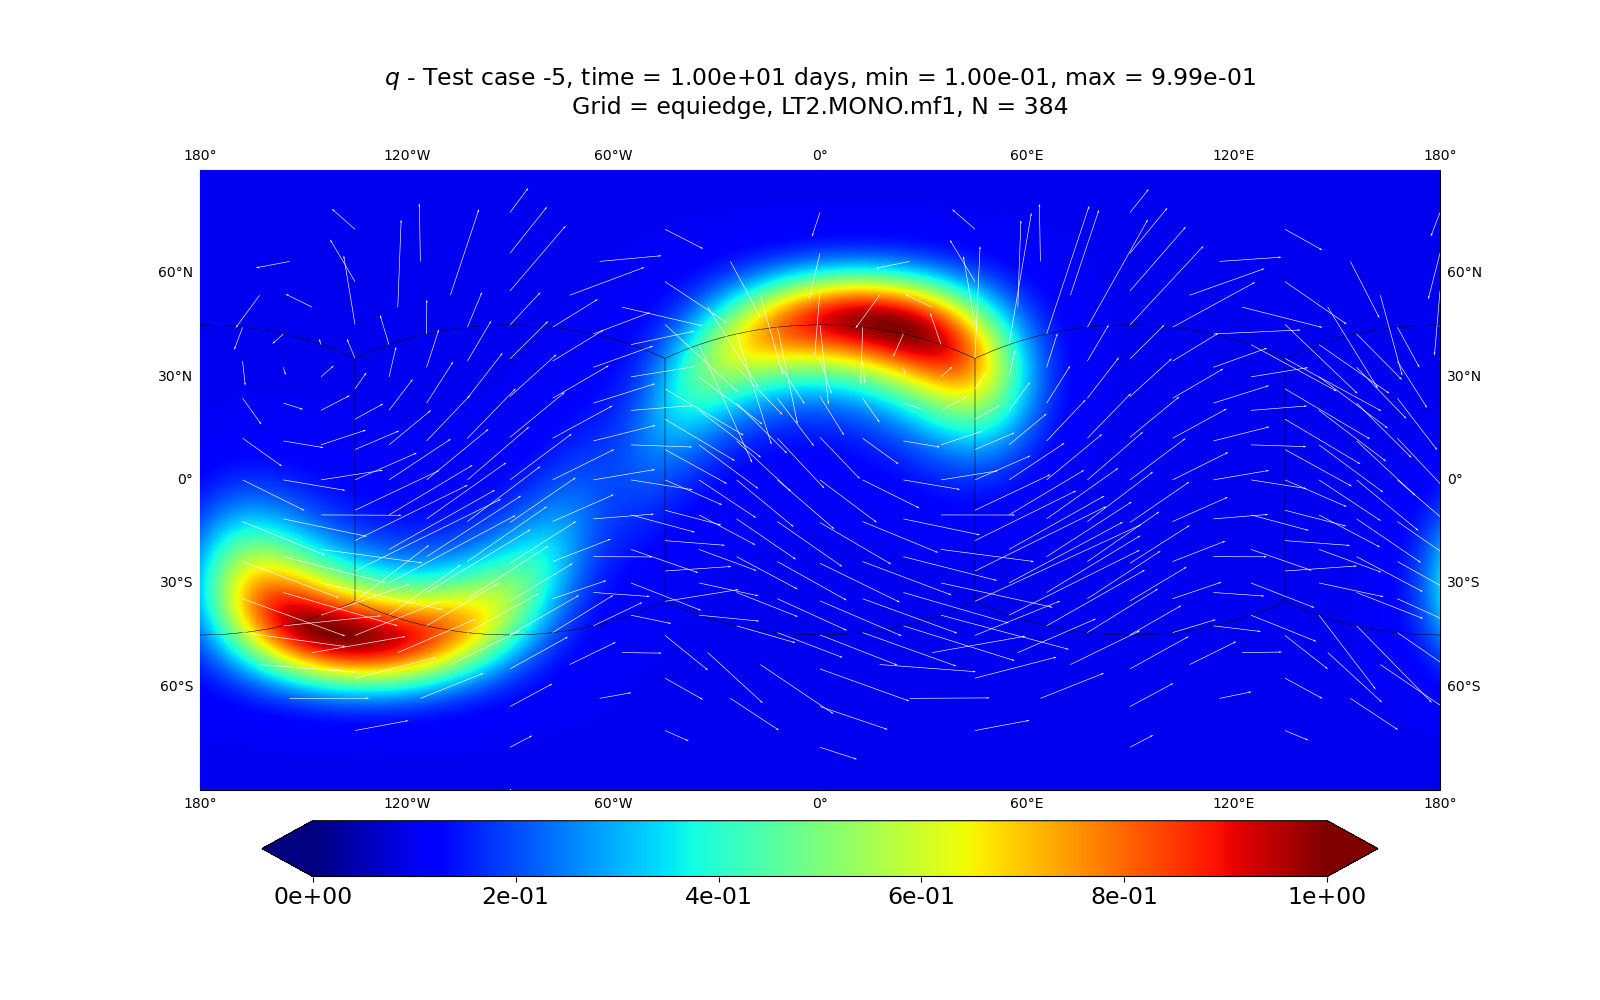
\includegraphics[width=1\linewidth]{h_tc-5_t10_alpha0_C384_g0_dg2_adv2_hord8_mf1_tf12}
		\caption{$t=10$ days.\label{chp-advcs-sec-exp-adv3-e}}
	\end{subfigure}
	\begin{subfigure}{0.45\textwidth}
		\centering
		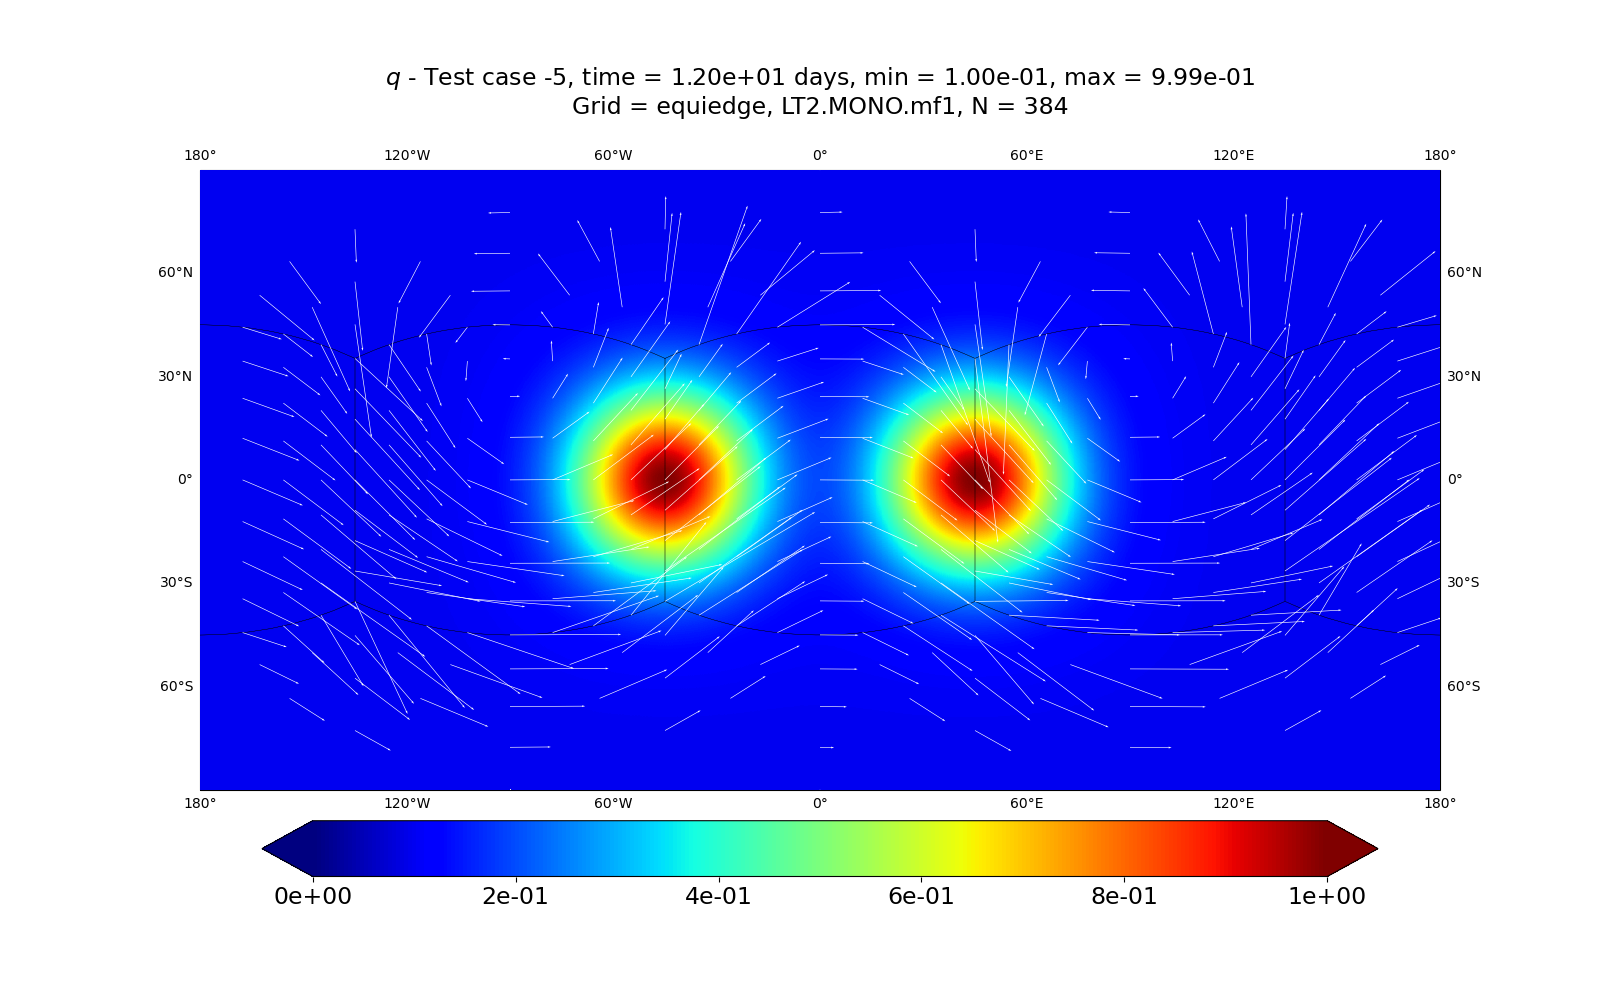
\includegraphics[width=1\linewidth]{h_tc-5_t12_alpha0_C384_g0_dg2_adv2_hord8_mf1_tf12}
		\caption{$t=12$ days.\label{chp-advcs-sec-exp-adv3-f}}
	\end{subfigure}
	\caption{Advection experiment results using the two Gaussian hills  (IC4, Table \ref{chp5-ic}) and 
		the variable in time divergent free wind (VF2, Table \ref{chp5-vf}).
		These figures show the advected profile after
		2 \eqref{chp-advcs-sec-exp-adv3-a}, 
		4  \eqref{chp-advcs-sec-exp-adv3-b},
		6  \eqref{chp-advcs-sec-exp-adv3-c},
		8  \eqref{chp-advcs-sec-exp-adv3-d},
		10  \eqref{chp-advcs-sec-exp-adv3-e},
		and 12  \eqref{chp-advcs-sec-exp-adv3-f} days.
		We are using the LT-MONO-mf1 scheme on the equi-edge grid (g0) with $N=384$.\label{chp-advcs-sec-exp-adv3}}
\end{figure}

\newpage
Figures \ref{chp-advcs-sec-exp-adv3-errors-0} and \ref{chp-advcs-sec-exp-adv3-errors-2} show 
the final error at a cube face for the equi-edge grid (g0) and the equiangular grid (g2), respectively.
The results without a mass fixer are very similar and are not shown here. 
We can observe that the errors for both PL and LT are very similar, and also the type of grid does not have a significant impact.

\begin{figure}[!htb]
	\centering
	\begin{subfigure}{0.45\textwidth}
		\centering
		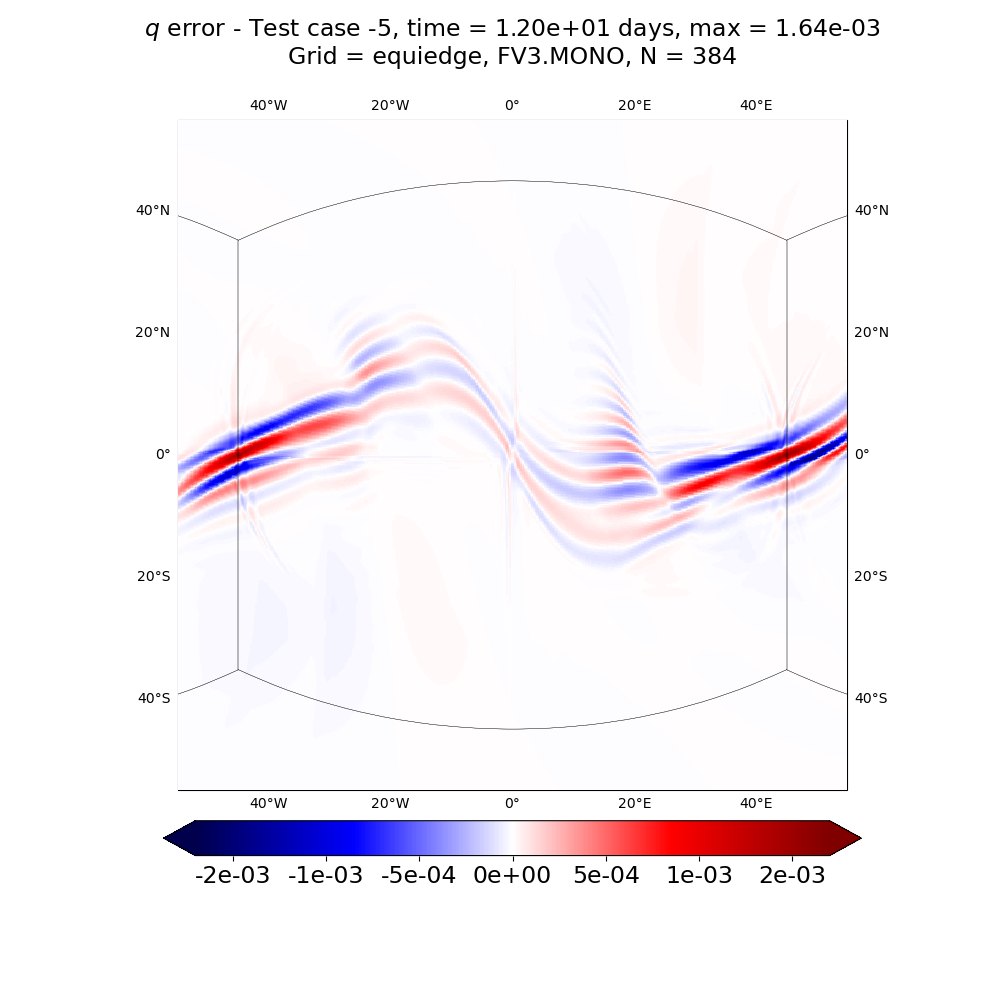
\includegraphics[width=1\linewidth]{h_error_tc-5_t12_alpha0_C384_g0_dg2_adv1_hord8_mf1_tf12}
		\caption{PL scheme.\label{chp-advcs-sec-exp-adv3-errors-0a}}
	\end{subfigure}
	\begin{subfigure}{0.45\textwidth}
		\centering
		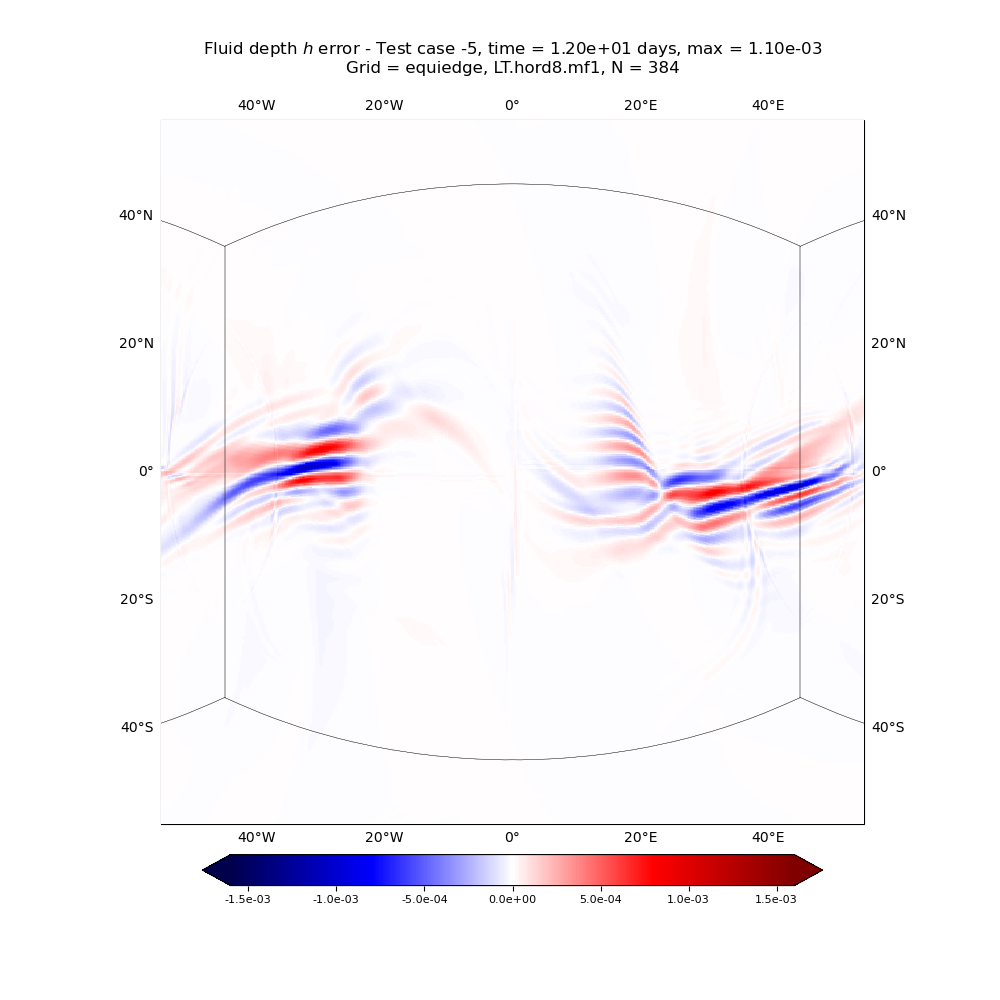
\includegraphics[width=1\linewidth]{h_error_tc-5_t12_alpha0_C384_g0_dg2_adv2_hord8_mf1_tf12}
		\caption{LT scheme.\label{chp-advcs-sec-exp-adv3-errors-0b}}
	\end{subfigure}
	\caption{
Advection experiment results using the two Gaussian hills  (IC4, Table \ref{chp5-ic}) and 
the variable in time divergence free wind (VF2, Table \ref{chp5-vf}).
These figures show the advected profile after
2 \eqref{chp-advcs-sec-exp-adv3-a}, 
4  \eqref{chp-advcs-sec-exp-adv3-b},
6  \eqref{chp-advcs-sec-exp-adv3-c},
8  \eqref{chp-advcs-sec-exp-adv3-d},
10  \eqref{chp-advcs-sec-exp-adv3-e},
and 12  \eqref{chp-advcs-sec-exp-adv3-f} days.
We are using the LT-MONO-mf1 scheme on the equi-edge grid (g0) with $N=384$.
		 \label{chp-advcs-sec-exp-adv3-errors-0}}
\end{figure}
\begin{figure}[!htb]
	\centering
	\begin{subfigure}{0.45\textwidth}
		\centering
		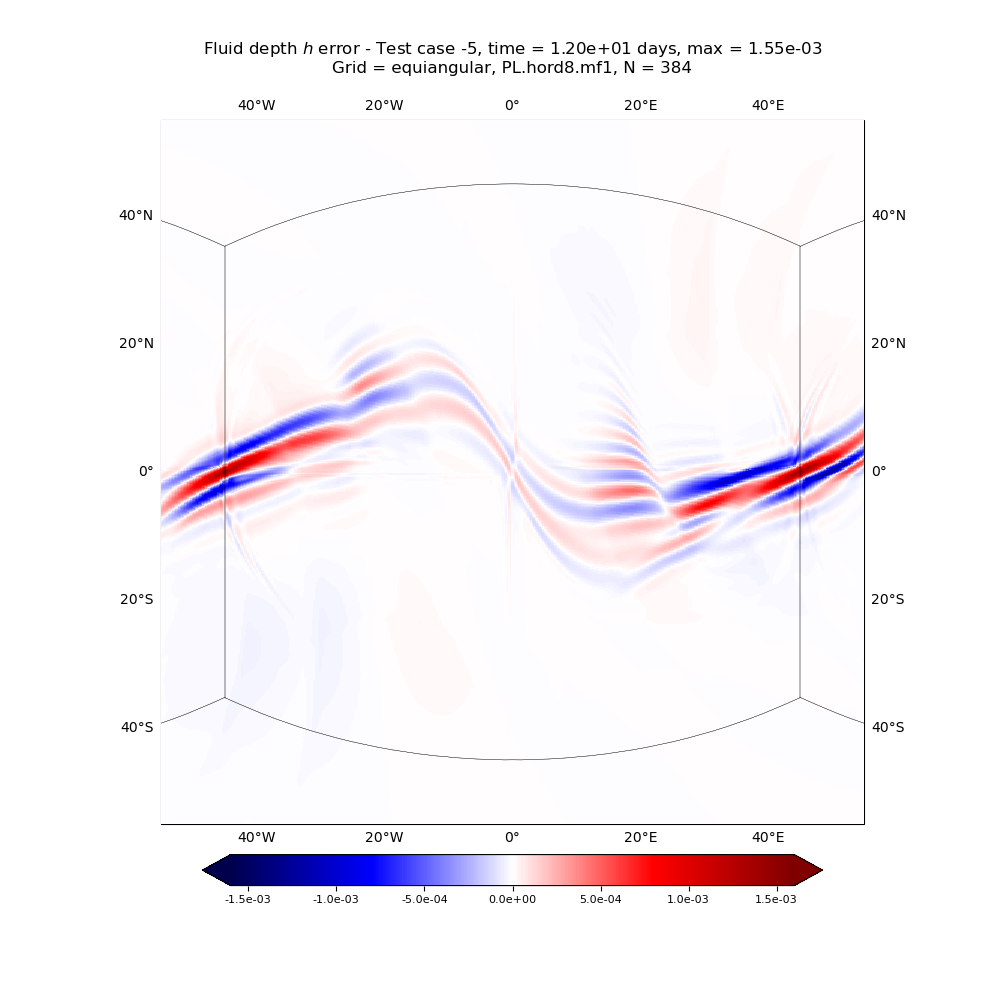
\includegraphics[width=1\linewidth]{h_error_tc-5_t12_alpha0_C384_g2_dg2_adv1_hord8_mf1_tf12}
		\caption{PL scheme.\label{chp-advcs-sec-exp-adv3-errors-2a}}
	\end{subfigure}
	\begin{subfigure}{0.45\textwidth}
		\centering
		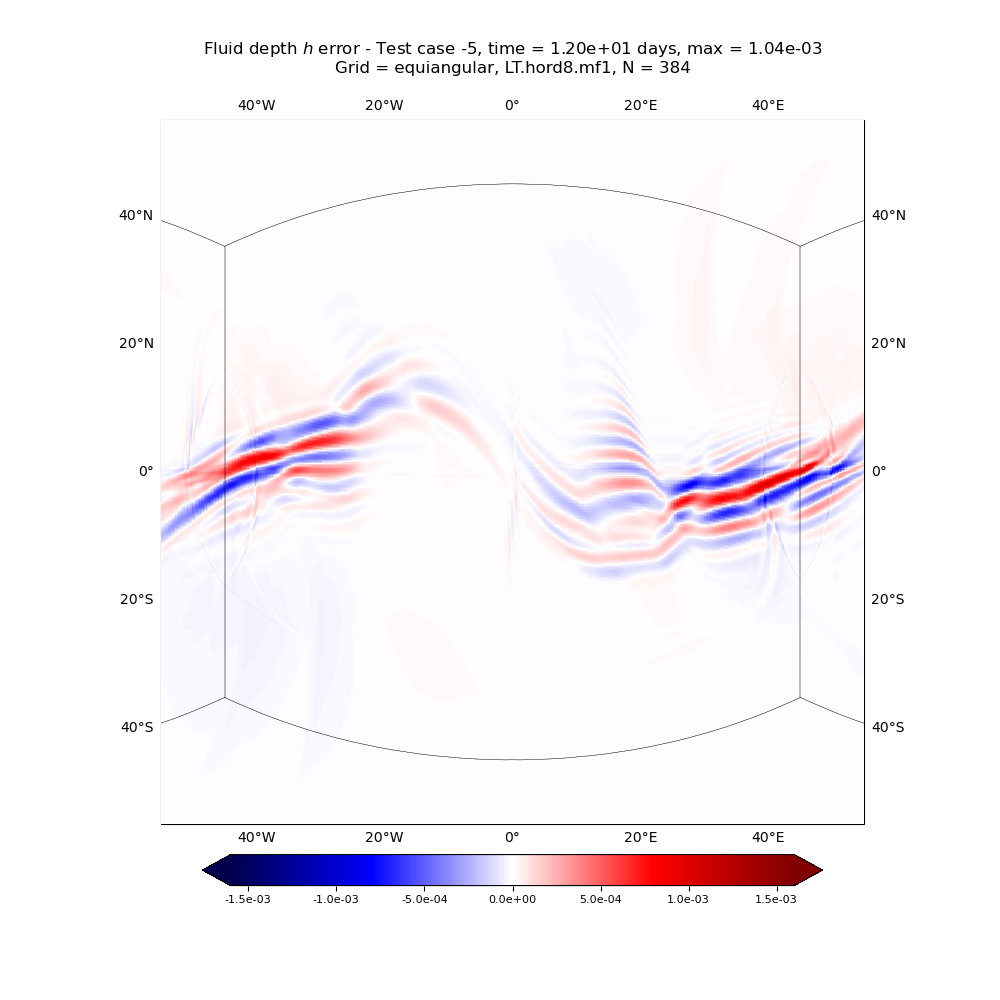
\includegraphics[width=1\linewidth]{h_error_tc-5_t12_alpha0_C384_g2_dg2_adv2_hord8_mf1_tf12}
		\caption{LT scheme.\label{chp-advcs-sec-exp-adv3-errors-2b}}
	\end{subfigure}
	\caption{As Figure \ref{chp-advcs-sec-exp-adv3-errors-0} but using the equiangular grid (g2).\label{chp-advcs-sec-exp-adv3-errors-2}}
\end{figure}
Figures \ref{chp-advcs-sec-exp-adv3-linf} and \ref{chp-advcs-sec-exp-adv3-l2} we show the error convergence in $L_{\infty}$ and $L_{2}$ norms.
Once more, it is evident that all schemes with the unlimited PPM (UNLIM) achieve second-order accuracy as expected, while those with the monotonic PPM (MONO) experience a reduced order 
in $L_{\infty}$ norm. In $L_{2}$ norm, the order is 2 for MONO.
Furthermore, LT and PL demonstrate almost the same errors when utilizing MONO, with the LT scheme being slightly smaller.
We also notice that the mass fixer does not impact the errors.

\begin{figure}[!htb]
	\centering
	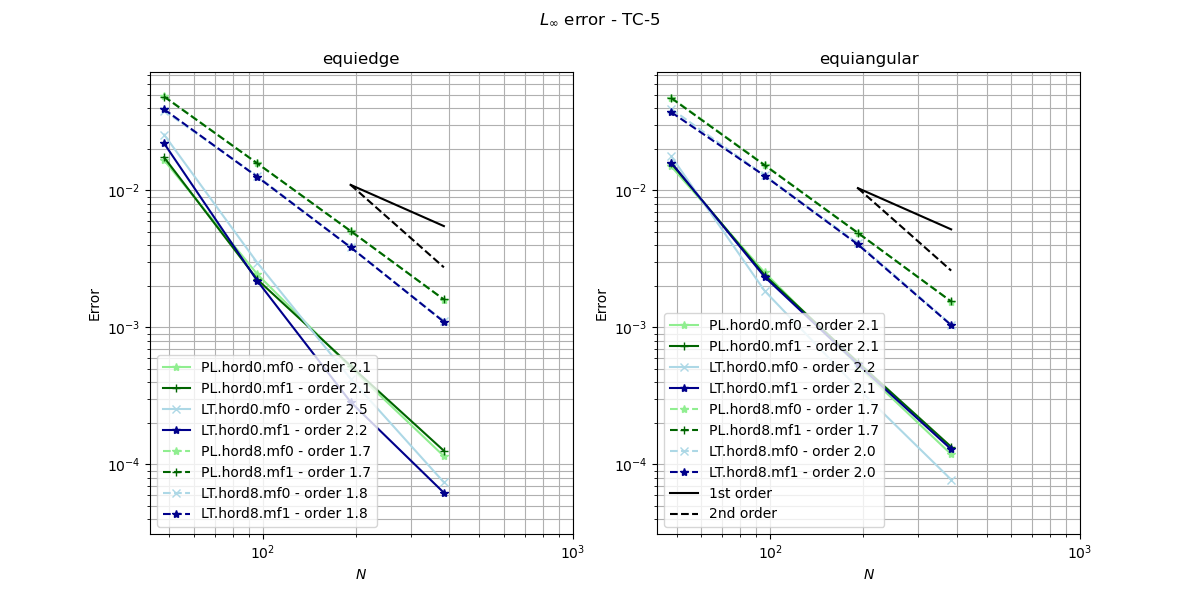
\includegraphics[width=1\linewidth]{linferror_tc-5_alpha0}
	\caption{
$L_{\infty}$ error convergence for the advection on the sphere test using the two Gaussian hills  (IC4, Table \ref{chp5-ic}) and the variable in time divergent-free wind
(VF2, Table \ref{chp5-vf}) on the equi-edge grid (g0, left) and on the equiangular grid (g2, right) after 12 days.
Blue lines indicate the use of the LT scheme, while green lines represent the PL scheme.
Solid lines represent the results with the unlimited PPM (UNLIM) scheme, whereas dashed lines represent the results with the monotonic PPM (MONO).
Light colors show the result without mass fixer (mf0), whereas dark colors show the results with flux averaging (mf1).
\label{chp-advcs-sec-exp-adv3-linf}}
\end{figure}

\begin{figure}[!htb]
	\centering
	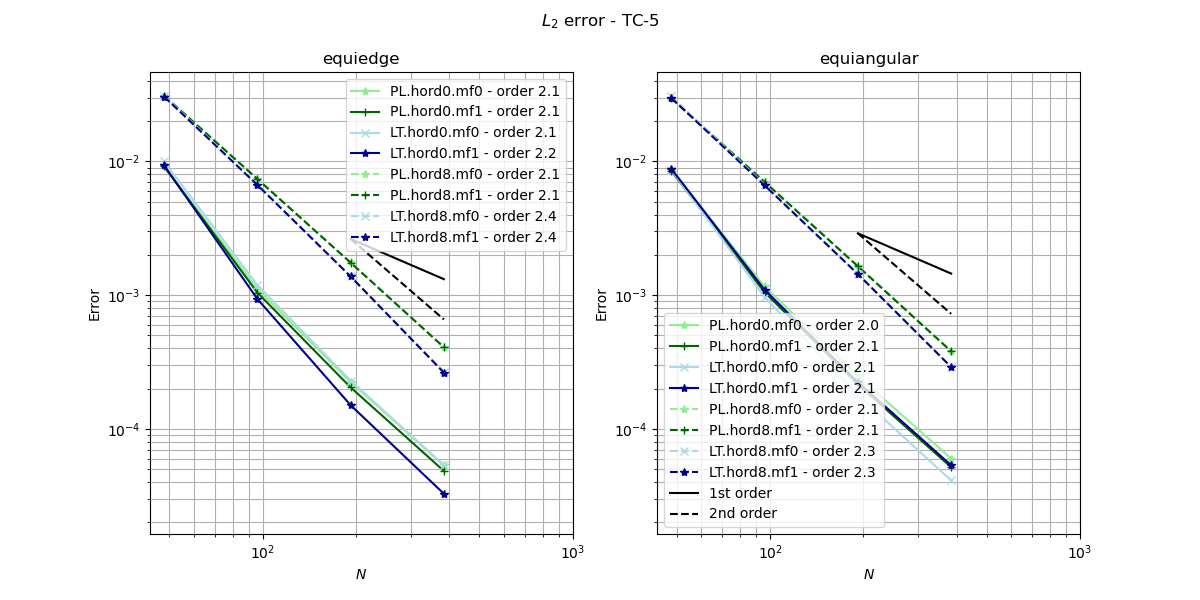
\includegraphics[width=1\linewidth]{l2error_tc-5_alpha0}
	\caption{As Figure \ref{chp-advcs-sec-exp-adv3-linf} but considering the $L_2$ norm. \label{chp-advcs-sec-exp-adv3-l2}}
\end{figure}


\newpage
\subsection{Divergent deformational flow}
The fifth and last test case considers the divergent wind VF3 from Table \ref{chp5-vf}, along with the initial condition IC4 from Table \ref{chp5-tab1}, 
where the velocity is time-dependent.
This test is also suggested by \citet{nair:2010}, and Figure \ref{chp-advcs-sec-exp-adv4} shows how the solution evolves over time.
Since the wind is divergent, we observe that it deforms the two Gaussian hills, creating new extrema.
Eventually, the final solution is equal to the initial condition after 12 days.
This test is the spherical analogous of the planar divergent deformational flow test presented in Section \ref{2d-adv-divflow}.
\begin{figure}[!htb]
	\centering
	\begin{subfigure}{0.45\textwidth}
		\centering
		\includegraphics[width=1\linewidth]{h_tc-6_t2_alpha0_C384_g0_dg2_adv2_hord8_mf1_tf12}
		\caption{$t=2$ days.\label{chp-advcs-sec-exp-adv4-a}}
	\end{subfigure}
	\begin{subfigure}{0.45\textwidth}
		\centering
		\includegraphics[width=1\linewidth]{h_tc-6_t4_alpha0_C384_g0_dg2_adv2_hord8_mf1_tf12}
		\caption{$t=4$ days.\label{chp-advcs-sec-exp-adv4-b}}
	\end{subfigure}

	\begin{subfigure}{0.45\textwidth}
		\centering
		\includegraphics[width=1\linewidth]{h_tc-6_t6_alpha0_C384_g0_dg2_adv2_hord8_mf1_tf12}
		\caption{$t=6$ days.\label{chp-advcs-sec-exp-adv4-c}}
	\end{subfigure}
	\begin{subfigure}{0.45\textwidth}
		\centering
		\includegraphics[width=1\linewidth]{h_tc-6_t8_alpha0_C384_g0_dg2_adv2_hord8_mf1_tf12}
		\caption{$t=8$ days.\label{chp-advcs-sec-exp-adv4-d}}
	\end{subfigure}

	\begin{subfigure}{0.45\textwidth}
		\centering
		\includegraphics[width=1\linewidth]{h_tc-6_t10_alpha0_C384_g0_dg2_adv2_hord8_mf1_tf12}
		\caption{$t=10$ days.\label{chp-advcs-sec-exp-adv4-e}}
	\end{subfigure}
	\begin{subfigure}{0.45\textwidth}
		\centering
		\includegraphics[width=1\linewidth]{h_tc-6_t12_alpha0_C384_g0_dg2_adv2_hord8_mf1_tf12}
		\caption{$t=12$ days.\label{chp-advcs-sec-exp-adv4-f}}
	\end{subfigure}
	\caption{
Advection experiment results using the two Gaussian hills  (IC4, Table \ref{chp5-ic}) and 
the divergent wind (VF3, Table \ref{chp5-vf}).
These figures show the advected profile after
2 \eqref{chp-advcs-sec-exp-adv4-a}, 
4  \eqref{chp-advcs-sec-exp-adv4-b},
6  \eqref{chp-advcs-sec-exp-adv4-c},
8  \eqref{chp-advcs-sec-exp-adv4-d},
10  \eqref{chp-advcs-sec-exp-adv4-e},
and 12  \eqref{chp-advcs-sec-exp-adv4-f} days.
We are using the LT-MONO-mf1 scheme on the equiangular grid (g2) with $N=384$. \label{chp-advcs-sec-exp-adv4}}
\end{figure}

Figures \ref{chp-advcs-sec-exp-adv4-errors-0} and \ref{chp-advcs-sec-exp-adv4-errors-2} show the final error at a cube face 
for the equi-edge grid (g0) and the equiangular grid (g2), respectively.
The results without a mass fixer are very similar and are not shown here. 
We can observe that the errors for PL are much larger, with significant errors present in many cells, whereas LT has smaller errors that are concentrated in some ripples.

\begin{figure}[!htb]
	\centering
	\begin{subfigure}{0.45\textwidth}
		\centering
		\includegraphics[width=0.9\linewidth]{h_error_tc-6_t12_alpha0_C384_g0_dg2_adv1_hord8_mf1_tf12}
		\caption{PL scheme.\label{chp-advcs-sec-exp-adv4-errors-0a}}
	\end{subfigure}
	\begin{subfigure}{0.45\textwidth}
		\centering
		\includegraphics[width=0.9\linewidth]{h_error_tc-6_t12_alpha0_C384_g0_dg2_adv2_hord8_mf1_tf12}
		\caption{LT scheme.\label{chp-advcs-sec-exp-adv4-errors-0b}}
	\end{subfigure}
	\caption{
		Advection experiment errors using the two Gaussian hills (IC4, Table \ref{chp5-ic}) and  the divergent wind (VF3, Table \ref{chp5-vf}) after 12 days, using the monotonic scheme (MONO)
	 with PL (left) and LT schemes (right) on the equi-edge grid (g0) with $N=384$.
	 \label{chp-advcs-sec-exp-adv4-errors-0}}
\end{figure}
\begin{figure}[!htb]
	\centering
	\begin{subfigure}{0.45\textwidth}
		\centering
		\includegraphics[width=0.9\linewidth]{h_error_tc-6_t12_alpha0_C384_g2_dg2_adv1_hord8_mf1_tf12}
		\caption{PL scheme.\label{chp-advcs-sec-exp-adv4-errors-2a}}
	\end{subfigure}
	\begin{subfigure}{0.45\textwidth}
		\centering
		\includegraphics[width=0.9\linewidth]{h_error_tc-6_t12_alpha0_C384_g2_dg2_adv2_hord8_mf1_tf12}
		\caption{LT scheme.\label{chp-advcs-sec-exp-adv4-errors-2b}}
	\end{subfigure}
	\caption{As Figure \ref{chp-advcs-sec-exp-adv4-errors-0} but using the equiangular grid (g2).\label{chp-advcs-sec-exp-adv4-errors-2}}
\end{figure}

Figures \ref{chp-advcs-sec-exp-adv4-linf} and \ref{chp-advcs-sec-exp-adv4-l2} we show the error convergence in $L_{\infty}$ and $L_{2}$ norms.
These figures highlight a major significant distinction between LT and PL schemes, unlike the previous tests.
It is clear that PL with the unlimited PPM achieves only first-order accuracy, whereas LT with the unlimited PPM (UNLIM) achieves third-order accuracy, 
surpassing second-order the expectation, for both equi-edge grid (g0) and the equiangular grid (g2) and norms.
For the monotonic  scheme (MONO), LT demonstrates second-order accuracy in the $L_2$ norm, while PL is only first-order.
LT with the monotonic scheme (MONO) exhibits smaller errors in the $L_{\infty}$ norm compared to the PL scheme for all grids.
This discrepancy arises because the PL splitting is designed for divergence-free flows, while LT is designed to be second-order regardless of the flow characteristics.
Finally, these results are similar to the planar divergent deformational flow test presented in Section \ref{2d-adv-divflow}.


\begin{figure}[!htb]
	\centering
	\includegraphics[width=0.9\linewidth]{linferror_tc-6_alpha0}
	\caption{
		$L_{\infty}$ error convergence for the advection on the sphere test using the two Gaussian hills  (IC4, Table \ref{chp5-ic}) and the divergent wind
		(VF3, Table \ref{chp5-vf}) on the equi-edge grid (g0, left) 
		and on the equiangular grid (g2, right) after 12 days.
		Blue lines indicate the use of the LT scheme, while green lines represent the PL scheme.
		Solid lines represent the results with the unlimited PPM (UNLIM) scheme, whereas dashed lines represent the results with the monotonic PPM (MONO).
		Light colors show the result without mass fixer (mf0), whereas dark colors show the results with flux averaging (mf1).
	\label{chp-advcs-sec-exp-adv4-linf}}
\end{figure}

\begin{figure}[!htb]
	\centering
	\includegraphics[width=0.9\linewidth]{l2error_tc-6_alpha0}
	\caption{As Figure \ref{chp-advcs-sec-exp-adv4-linf} but considering the $L_2$ norm. \label{chp-advcs-sec-exp-adv4-l2}}
\end{figure}

\newpage
\section{Concluding remarks}
\label{chp-cs-conc}
In summary, in this Chapter, we demonstrate how the dimension-splitting methods from Chapter \ref{chp-2d-fv}, 
namely the PL and LT methods, can be extended to the cubed-sphere to solve the advection equation on the sphere 
using the cubed-sphere grids equi-edge (g0) and equiangular (g2), along with the duo-grid interpolation presented in Chapter \ref{chp-cs-grids}.
We observed a major difference in the metric term that appears in this case, and it may be treated differently in the PPM flux computation.
Also, on the cubed-sphere, we need to apply a mass fixer, namely averaging the fluxes at the cube edges, to ensure exact mass preservation.

We showed that LT may use a more accurate metric term formulation, since this scheme is more flexible and does not need to eliminate the splitting error for a constant
scalar wind and divergence-free wind, which is demanded for the PL scheme.
This difference in requirements allows the LT scheme to utilize a more accurate metric term formulation compared to PL.


The conclusions of this Chapter are essentially extensions of the results from Chapter \ref{chp-2d-fv} from the plane to the cubed-sphere.
In fact, the LT scheme, which utilize a second-order departure point calculation, showed to have smaller errors than the PL scheme,
which is designed to preserve a constant scalar field for divergence-free winds.
Both schemes are second-order when no limiter is employed and the wind is divergence-free.
The major difference between LT and PL is when the wind is not divergence-free.
In this case, PL is only first order, while LT is second-order. Even with a limiter, LT is much more accurate than PL in this case.
This was demonstrated consistently throughout the simulations.
Therefore, our major conclusion here is that the LT scheme is much more accurate regardless of whether the wind is divergence-free or not, while 
PL is only accurate for divergence-free winds.

Additionally, the Gaussian hill and cosine bell advection through a rotated zonal wind showed 
that some errors of PL and LT presented small spikes whenever the Gaussian hill passed over a corner.
The overall results for this test showed that the LT scheme have slightly smaller errors.
We could also observe that the mass fixer did not significantly impact the results,
and the equi-edge grid (g0) grid generally exhibited smaller errors compared to the equiangular grid (g2), with LT showing good performance in both grids.
